\section{Introduction}

Canonical correlation analysis (CCA) is a joint multidimensional dimensionality reduction
algorithm for exactly two datasets \cite{hotelling1936relations}. CCA finds a
linear transformation for each dataset such that the correlation between the
two transformed features is maximized. While CCA itself is not a data fusion
algorithm, the correlated features that it returns may be used in data fusion algorithms.
Such data fusion algorithms are becoming a necessity with the increased ability to capture
high-dimensional multi-modal datasets, arising in fields such as computer vision
\cite{hardoon2004canonical, dhillon2011multi, melzer2001nonlinear, zhai2015instance,
  lisanti2014matching,ahsan2014clustering,hardoon2006correlation,chaudhuri2009multi},
medical signal processing, \cite{deleus2011functional, arbabshirani2010comparison,
  khalid2013improving,guccione2013functional, correa2010canonical, lin2013identifying,
  seoane2014canonical, lin2013group, zhang2013l1, nakanishi2014enhancing,
  zhang2014frequency, spuler2013spatial, campi2013non, chen2014removal,
  kuzilek2014comparison}, economics \cite{todros2012measure}, climatology
\cite{wilks2014probabilistic, prera2014using, steward2014assimilating}, and classical
signal processing like Wiener filters \cite{scharf1998wiener}, array processing
\cite{ge2009does}, and cognitive radio \cite{manco2014kernel}.

At the heart of the CCA algorithm is a SVD of a matrix product involving the individual
covariance matrices of the datasets and the cross-covariance matrix between them. When
these matrices are known \textit{a priori}, the non-zero singular values of this matrix
represent correlated components between the datasets. These singular values are bounded
between zero and one; a larger singular value indicates a stronger correlation. However,
in all of the above applications, the true covariance matrices are unknown and must be
estimated from data. When using CCA with sample covariance estimates from fewer samples
than the combined dimensions of the datasets, the largest singular value of this matrix is
deterministically one \cite{pezeshki2004empirical}, falsely reporting a perfect
correlation between the datasets. In this low-sample, high-dimensionality regime, CCA
fails to reliably detect correlations between the datasets and because of this, many have
abandoned CCA as a correlation analysis tool.

This chapter shows that detecting correlations in this low-sample high-dimensionality
regime is feasible. We first empirically showcase the performance loss of CCA in this
regime, provide a statistical significance test for CCA correlations, and derive a
consistency bound that elucidates when this test can reliably detect correlations. We then
present informative CCA (ICCA), which uses insights from random matrix theory to first
trim the number of components used in the singular value decomposition used in CCA
\cite{nadakuditi2011fundamental}. We provide a similar statistical test and consistency
bound for ICCA and showcase that it is able to reliably detect correlations in the sample
deficient regime. Importantly, we see that while the consistency boundary for CCA depends
on the correlation between the datasets, the ICCA consistency boundary is independent of
the underlying correlation.

This chapter assumes that each dataset is modeled with a low-rank signal-plus-noise data
model, which is ubiquitous in signal processing applications. Surprisingly, the
performance of CCA has not been extensively studied for this data model and therefore we
use this chapter to complete the discussion by examining the data model in the presence of
missing data. To showcase the improved performance of ICCA, we create three real-world
audio-video datasets. We note that depending on the application, the linear, low-rank
signal-plus-noise data model may be inappropriate. In such a setting, kernel CCA (KCCA)
\cite{welling2005kcca,yu2007learning}, uses the kernel trick to map the data into a higher
dimensional space. We leave the performance analysis of such kernel methods for non-linear
data models as important future work.

This chapter is organized as follows. We provide the linear low-rank signal-plus-noise
data model in Section \ref{sec:chpt4:model}. We then derive the solution of CCA in Section
\ref{sec:chpt4:cca} and show how to estimate the number of correlated components from its
solution. In Section \ref{sec:chpt4:emp_cca}, we derive the empirical version of CCA using
sample covariance matrices and discuss the standard Wilk's Lambda Test for correlation
detection. This derivation gives rise to the ICCA algorithm. We then provide statistical
tests to estimate the number of correlated components between the datasets for both CCA
and ICCA. We provide previous known results for empirical CCA in Section
\ref{sec:chpt4:cca_theory} and then state and prove new results for CCA and ICCA
consistency in Section \ref{sec:chpt4:new_results}. In Section \ref{sec:chpt4:missing}, we
extend the consistency analysis to the missing data setting and provide an analogous
consistency bound. Finally, we verify our theorems both on simulated data and real-world
datasets in Section \ref{sec:chpt4:emp}.


\section{Data Model}\label{sec:chpt4:model}

Let $\xii\in\complex^{p\times 1}$ and $\yii\in\complex^{q\times 1}$ be modeled as
\beq\ba\label{eq:chpt4:data_model}
&\xii = \Ux\sx + \zx\\
&\yii = \Uy\sy + \zy,\\
\ea\eeq
where $\Ux^H\Ux=I_{\kx}$, $\Uy^H\Uy=I_{\ky}$, $\zx\simiid\mathcal{CN}(0,I_p)$ and
$\zy\simiid\mathcal{CN}(0,I_q)$. Furthermore, assume that
\be\ba
&\sx\sim\mathcal{CN}(0,\Tx)\\
&\sy\sim\mathcal{CN}(0,\Ty),\\
\ea\ee
where $\Tx=\diag\left(\left(\tx_1\right)^2,\dots,\left(\tx_{\kx}\right)^2\right)$ and
$\Ty=\diag\left(\left(\ty_{1}\right)^2,\dots,\left(\ty_{\ky}\right)^2\right)$. Assume that
$\zx$ and $\zy$ are 
mutually independent and independent from both $\sx$ and $\sy$. Finally, assume that
\be
\E{\sx \sy^H} \defeq \Kxy = \Tx^{1/2}\Pxy\Ty^{1/2}
\ee
where the entries of $\Pxy$ are $-1\leq \rho_{kj} \leq 1$ and represent the correlation
between $\sx^{(k)}$ and $\sy^{(j)}$. For reasons to be made clear later, define 
\be
\Kxytil = \left(\Tx+I_{\kx}\right)^{-1/2}\Kxy\left(\Ty+I_{\ky}\right)^{-1/2}
\ee
and define the singular values of $\Kxytil$ as
$\kappa_1,\dots,\kappa_{\min(\kx,\ky)}$. Under this model, we define the following 
covariance matrices  
\beq\label{eq:chpt4:true_scm}\ba
&\E{\xii\xii^H} = \Ux\Tx\Ux^H + I_p \defeq \Rxx\\
&\E{\yii\yii^H} = \Uy\Ty\Uy^H + I_q \defeq \Ryy\\
&\E{\xii\yii^H} = \Ux\Kxy\Uy^H \defeq \Rxy.\\
\ea\eeq

\begin{Assum}\label{assum:chpt4:noise}
Let $Z_x^{(n)} = [z_{x,1},\dots,z_{x,n}]$ be the $p\times n$ matrix formed by stacking $n$
observations of our noise. Let $Z_x^{(n)}$ have singular values
$\sigma_1\left(Z_x^{(n)}\right)\geq\cdots\geq\sigma_p\left(Z_x^{(n)}\right)$. Let
$\mu_{Z_x^{(n)}}$ be the empirical singular value distribution defined by the probability
  measure
\be
\mu_{Z_x^{(n)}} = \frac{1}{p}\sum_{i=1}^p \delta_{\sigma_i\left(Z_x^{(i)}\right)}.
\ee
We assume that the probability measure $\mu_{Z_x^{(n)}}$ converges almost surely weakly as
$p,n\to\infty$ with $p/n\to c_x$ to a non-random compactly supported probability measure
$\mu_{Z_x}$ that is supported on $[a_x,b_x]$. We assume that $\sigma_1\convas b_x$. 

Similarly, we assume that the empirical singular value distribution for the noise matrix
of $Y$ converges almost surely to the non-random compactly supported probability measures
$\mu_{Z_y}$ that is supported on $[a_y,b_y]$ and that $\sigma_1\convas b_y$.
\end{Assum}

\section{Canonical Correlation Analysis}\label{sec:chpt4:cca}

Canonical Correlation Analysis (CCA) is a dimensionality reduction algorithm that finds
linear transformations for $\xii$ and $\yii$ such that in the projected spaces, the
transformed variables
are maximally correlated. Specifically, CCA solves the following optimization problem
\beq\label{eq:chpt4:opt_cca}
\rhocca =\argmax_{\wx,\wy} \frac{\wx^H\Rxy\wy}{\sqrt{\wx^H\Rxx\wx}\sqrt{\wy^H\Ryy\wy}},
\eeq
where $\wx$ and $\wy$ are called canonical vectors and $\rhocca$ is called the canonical
correlation coefficient. Notice that we can scale $\wx$ and
$\wy$ and still achieve the same objective function. Therefore, we may constrain the
canonical variates to have unit norm, resulting in 
\beq\label{eq:chpt4:cca}\ba
&\argmax_{\wx,\wy} &&\wx^H\Rxy\wy\\
&\text{subject to} && \wx^H\Rxx\wx = 1\\
&&& \wy^H\Ryy\wy=1.\\
\ea\eeq
Substituting the change of variables $\wxt=\Rxx^{1/2}\wx$ and
$\wyt=\Ryy^{1/2}\wy$ in (\ref{eq:chpt4:cca}) results in the following optimization problem
\beq\label{eq:chpt4:cca_svd}\ba
&\argmax_{\wxt,\wyt} &&\wxt^H\Rxx^{-1/2}\Rxy\Ryy^{-1/2}\wyt\\
&\text{subject to} && \wxt^H\wxt = 1\\
&&& \wyt^H\wyt=1.\\
\ea\eeq
Examining the optimization problem in (\ref{eq:chpt4:cca_svd}), we can immediately see that the
solution to CCA may be solved via the SVD of the matrix
\beq\label{eq:chpt4:c_cca}
\Ccca = \Rxx^{-1/2}\Rxy\Ryy^{-1/2}. 
\eeq
Define $\Ccca=FKG^T$ as the SVD of $\Ccca$ where $F$ is an unitary
$p\times p$ matrix with columns $f_1,\dots,f_p$, $G$ is a unitary $q\times q$ matrix with
columns $g_1,\dots,g_q$, and
$K=\diag(k_1,\dots,k_{\min(p,q)})$ is a $p\times q$ matrix whose diagonal elements are the
singular values of $\Ccca$. Therefore, the solution to (\ref{eq:chpt4:cca_svd}) is
\be\ba
\wxt = f_1\\
\wyt = g_1\\
\rho_{\text{cca}} = k_1.\\ 
\ea\ee
We can obtain higher order canonical correlations and vectors by taking sucessive singular
value and vector pairs. From this solution, it is clear that the number of non-zero
canonical correlation coefficients is exactly equal to the rank of $\Ccca$. Noticing that
$\Rxx$ and $\Ryy$ are non-singular and recalling the definition of $\Rxy$, we have that
\be\ba
&\text{\# canonical correlation coefficients}&&=\rank(\Ccca)\\
&&& = \rank(\Rxx^{-1/2}\Rxy\Ryy^{-1/2})\\
&&& = \rank(\Rxy)\\
&&& = \rank(\Kxy)\\
&&&\defeq k.\\
\ea\ee
Therefore, when we know all parameters, $k$ is exactly the number of non-zero singular
values of $\Kxy$. We note that $k\leq\min(\kx,\ky)$.

\section{Empirical CCA for Correlation Detection}\label{sec:chpt4:emp_cca}
In many applications, we do not know the covariance matrices $\Rxx$, $\Ryy$, and $\Rxy$
\textit{a priori}. In this section, we assume that all parameters in
(\ref{eq:chpt4:data_model}) are unknown. Therefore, we cannot simply determine the number
of canonical correlation coefficient by examining the rank of $\Rxy$. Instead, we are
given multiple observations of each dataset that we stack columnwise to form the data
matrices
\be\ba
& X = [x_1,\dots,x_n]\\
& Y = [y_1,\dots,y_n],\\
\ea\ee
where for $i=1,\dots,n$, $\xii$ and $\yii$ are modeled in (\ref{eq:chpt4:data_model}). It
is important to note that the number of observations of each dataset must be the same and
that the observations come in pairs. Defining
$\Zx = [z_{x,1},\dots,z_{x,n}]$, $\Zy = [z_{y,1},\dots,z_{y,n}]$,
$\Vx=[s_{x,1},\dots,s_{x,n}]^H$, and $\Vy=[s_{y,1},\dots,s_{y,n}]$, we may write our data
matrices as the sum of a low-rank signal matrix and noise matrix
\beq\label{eq:chpt4:data_matrices}\ba
& X = \Ux\Vx^H + \Zx\\
& Y = \Uy\Vy^H + \Zy.
\ea\eeq
Given
these data matrices, we form estimates of our unknown covariance matrices via 
\be\ba
& \Rxxhat = \frac{1}{n}XX^H\\
& \Ryyhat = \frac{1}{n}YY^H\\
& \Rxyhat = \frac{1}{n}XY^H.\\
\ea\ee
Define the data SVDs
\be\ba
& X = \Uxhat\Sigxhat\Vyhat^H\\
& Y = \Uyhat\Sigyhat\Vyhat^H\\
\ea\ee
and trimmed matrices
\be\ba
& \Uxtil = \Uxhat\left(:,1:\min(p,n)\right)\\
& \Vxtil = \Vxhat\left(:,1:\min(p,n)\right)\\
& \Uytil = \Uyhat\left(:,1:\min(q,n)\right)\\
& \Vytil = \Vyhat\left(:,1:\min(q,n)\right).\\
\ea\ee
Given these definitions, substituting the sample covariance estimates into $\Ccca$ yields
the estimate
(see \cite{nadakuditi2011fundamental})
\be
\Cccahat = \Uxtil\Vxtil^H\Vytil\Uytil^H.
\ee
We denote the singular values of this matrix for $j=1,\dots,\min(p,q)$ $\rhohatcca^{(j)}$,
which are the empirical CCA correlation coefficient estimates. Empirical CCA can return up
to $\min(p,q)$ canonical correlations, however, we know from the data model in
(\ref{eq:chpt4:data_model}) that $X$ and $Y$ have $\kx$ and $\ky$ underlying signals,
respectively. As $\kx$ and $\ky$ are unknown, let $\kxhat$ and $\kyhat$ be estimates of
the number of underlying signals in each dataset. It is common to return only
$\min(\kxhat,\kyhat)$ canonical correlations. Therefore, define the top
$\min(\kxhat,\kyhat)$ singular values of $\Cccahat$ as 
\beq\label{eq:chpt4:rhohatcca}
\rhohatcca^{(1)},\dots,\rhohatcca^{(\min(\kxhat,\kyhat))}.
\eeq
For now, we assume that we are given $\kxhat$ and $\kyhat$, but we will return to the
problem of estimating these parameters from data. To estimate the canonical vectors, we
use the corresponding left and right singular vectors of $\Cccahat$, $f_i$ and $g_i$ to
form 
\beq\label{eq:chpt4:cca_vects}\ba
& w_x^{(i)} = \Rxxhat^{-1/2}f_i\\
& w_y^{(i)} = \Ryyhat^{-1/2}f_i.\\
\ea\eeq 


\subsection{Classical Wilks Lambda Correlation Test}\label{sec:chpt4:wilks}
To test the significance of the empirical CCA canonical correlation estimates, classical
methods \cite{hardle2007applied} employ the Wilks likelihood ratio statistic, 
\be
\prod_{i=1}^k \left(1 - \left(\rhohatcca^{(i)}\right)^2\right).
\ee
However, the distribution of this statistic is very unwieldy. For large $n$ it is common
to instead use the statistic \cite{bartlett1954note}
\be
\Lambda\left(\rhohatcca^{(1)},\dots,\rhohatcca^{(\min(p,q))}\right) = -\left(n-\frac{p+q
    +3}{2}\right)\log\left(\prod_{i=1}^k\left(1-\rhohatcca^{(i)2}\right)\right)
\ee
because this test statistic approximately follows a chi-square distribution
\be
\Lambda\left(\rhohatcca^{(1)},\dots,\rhohatcca^{(\min(p,q))}\right)\sim\chi_{pq}^2. 
\ee
This statistic tests whether the first canonical correlation, $\rhohatcca^{(1)}$, is
significant (i.e. whether the two datasets are uncorrelated). To determine significance, we
compare the statistic against a threshold to achieve a desired false alarm rate via
\beq\label{eq:chpt4:wilks}
\Lambda\left(\rhohatcca^{(1)},\dots,\rhohatcca^{(\min(p,q))}\right) \siggtrless \eta,
\eeq
where $\eta = Q^{-1}_{\chi_{pq}^2}\left(1-\alpha\right)$, $\alpha$ is a desired
probability of false alarm and $Q$ is the inverse cumulative distribution function of the
chi squared distribution with $p\times q$ degrees of freedom. To
test the significance of successive empirical CCA correlation estimates, we modify the
statistic to  
\be
\Lambda\left(\rhohatcca^{(s+1)},\dots,\rhohatcca^{(\min(p,q))}\right) = -\left(n-\frac{p+q
    +3}{2}\right)\log\left(\prod_{i=s+1}^k\left(1-\rhohatcca^{(i)2}\right)\right),
\ee
which is approximately
\be
\Lambda\left(\rhohatcca^{(s+1)},\dots,\rhohatcca^{(\min(p,q))}\right)\sim\chi_{(p-s)(q-s)}^2. 
\ee
Comparing this statistic to an appropriate threshold tests whether the first $s+1$
canonical correlation are significant. 

\subsection{Informative CCA (ICCA)}

When the number of samples is less than the combined dimension of the datasets ($n<p+q$),
the largest singular value of $\Cccahat$ is deterministically one
\cite{pezeshki2004empirical}, regardless of whether an underlying correlation actually
exists between the datasets. This observation led Pezeshki and Scharf et al. to correctly
conclude that in this regime
\begin{quote}
    ... the empirical canonical correlations are defective and
      may not be used as  estimates of canonical correlations between random
    variables.
\end{quote}
This is a very unfortunate property of empirical CCA as many of the motivating
applications operate in this low-sample, high-dimensionality regime. A key observation by
\cite{nadakuditi2011fundamental} shows that the singular values of $\Cccahat$ are exactly
the same as the singular values of $\Vxtil^H\Vytil$. This is a $\min(p,n)\times\min(q,n)$
matrix that uses all right singular vectors of each dataset corresponding to a non-zero
singular value. However, under the low-rank signal-plus-noise model,
\cite{nadakuditi2011fundamental} shows that only a few of the right singular vectors
actually contain \textit{informative} signal. Therefore, by trimming $\Vxtil$ and $\Vytil$
to have only $\kxhat$ and $\kyhat$ columns, we can avoid the performance loss of CCA in
the sample deficient regime. Define the trimmed data SVDs
\beq\label{eq:chpt4:trimmed_svds}\ba
& \Uxcir = \Uxhat\left(:,1:\kxhat\right)\\
& \Vxcir = \Vxhat\left(:,1:\kxhat\right)\\
& \Uycir = \Uyhat\left(:,1:\kyhat\right)\\
& \Vycir = \Vyhat\left(:,1:\kyhat\right).\\
\ea\eeq
Given these definitions, we define the informative CCA (ICCA) matrix
\be
\Ciccahat = \Uxcir\Vxcir^H\Vycir\Uycir^H.
\ee
Similar to CCA, define the top $\min(\kxhat,\kyhat)$ singular values of $\Ciccahat$ as,
\beq\label{eq:chpt4:rhohaticca}
\rhohaticca^{(1)},\dots,\rhohaticca^{(\min(\kxhat,\kyhat))}.
\eeq
To estimate the canonical vectors, we
use the corresponding left and right singular vectors of $\Ciccahat$, $f_i$ and $g_i$ to
form 
\beq\label{eq:chpt4:icca_vects}\ba
& w_x^{(i)} = \Rxxhat^{-1/2}f_i\\
& w_y^{(i)} = \Ryyhat^{-1/2}f_i.\\
\ea\eeq 
\subsection{New Statistical Tests for Correlation Detection}
 Given the canonical correlation estimates from CCA and ICCA, we can
estimate the number of canonical correlations using the test statistics
\beq\label{eq:chpt4:khats}\ba
& \khatcca = \sum_{i=1}^{\min(p,q)} \indicator_{\left\{\left(\rhohatcca^{(i)}\right)^2 >\taucca\right\}}\\
& \khaticca = \sum_{i=1}^{\min(\kxhat,\kyhat)} \indicator_{\left\{\left(\rhohaticca^{(i)}\right)^2 >\tauicca\right\}},\\
\ea\eeq
where $\indicator_{\left\{\cdot\right\}}$ is the indicator function and
\beq\label{eq:chpt4:taus}\ba
& \taucca = F^{-1}_{\text{cca}}(1-\alpha)\\
& \tauicca = F^{-1}_{\text{icca}}(1-\alpha).\\
\ea\eeq
Here $F_{\text{cca}}$ and $F_{\text{icca}}$ are the distributions of the square of the largest singular
value of $\Cccahat$ and $\Ciccahat$ for the null setting where $\Vxtil$ and $\Vytil$ are the
$\min(n,p)$ and $\min(n,q)$ columns of two independent Haar (or isotropically random)
distributed $n\times n$ matrices. The exact distribution of the squared singular values of
$\Cccahat$ and $\Ciccahat$ in
the null model is given in \cite{constantine1976asymptotic}. The distributions of the
square of the largest singular value of $\Cccahat$ and $\Ciccahat$ in the null model may be
approximated to second-order by the Tracy-Widom law \cite{johnstone2008multivariate} as
\be\ba
&\taucca \approx \sigma_{n,p,q}\twc^{-1}(1-\alpha) + \mu_{n,p,q},\\
&\tauicca \approx \sigma_{n,\kxhat,\kyhat}\twc^{-1}(1-\alpha) + \mu_{n,\kxhat,\kyhat},\\
\ea\ee
where $\sigma_{n,p,q}$ is a scaling parameter and $\mu_{n,p,q}$ is a centering
parameter. See Appendix D for values of these parameters as well as a derivation of the
Tracy-Widom distribution for CCA and ICCA. The appendix also plots the accuracy of the
Tracy-Widom approximation for CCA and ICCA for finite sized systems.

\section{Empirical CCA Theory}\label{sec:chpt4:cca_theory}

In this section, we provide important, but previous results about empirical CCA. The first
proposition specifically quantifies the conditions on when the largest canonical
correlation reported by empirical CCA is deterministically one. 

\begin{prop}\label{prop:pezeshki}
Let $n,p,q\to\infty$ such that $p/n\to c_x$ and $q/n\to c_y$. Let $p+q\leq n$. Then the
largest singular value of $\Cccahat$ generated from data modeled in (\ref{eq:chpt4:data_model})
behaves as 
\be
\rhohatcca^{(1)} = 1.
\ee
\end{prop}
\begin{proof}
See \cite{pezeshki2004empirical}.
\end{proof}

This important result shows that the canonical correlation estimates of empirical CCA in
the sample deficient regime are unable to detect the presence of correlation between
datasets. The proof of this proposition motivates the ICCA algorithm. 

The second proposition provides the limiting behavior of the empirical canonical
correlations. This very recent result makes contact with a natural phase transition, below
which the empirical canonical correlations behave as if the underlying datasets were noise
only. Below, we provide a proof to transform our data model in (\ref{eq:chpt4:data_model})
to the one used in the original theorem. Because this is such a new result, we provide an
similar proof in Appendix C using our own notation. A key insight to this result is that
the phase transition boundary is dependent on the underlying correlations between the
datasets, which is an another undesirable property of CCA. 

\begin{prop}
Let $n,p,q\to\infty$ such that $p/n\to c_x$ and $q/n\to c_y$. Assume that $p+q<n$. For
$i=1,\dots,\min(\kx,\ky)$ let $\rhohatcca^{(i)}$ be the largest singular singular values
of $\Cccahat$ generated from data modeled in (\ref{eq:chpt4:data_model}). Then these singular
values behave as 
\beq\label{eq:chpt4:bao_cca}
\rhohatcca^{(i)} \convas \begin{cases} \sqrt{\kappa_i^2\left(1-c_x+\frac{c_x}{\kappa_i^2}\right)\left(1-c_y+\frac{c_y}{\kappa_i^2}\right)} & \kappa_i^2 \geq r_c \\ \sqrt{d_r} &\kappa_i^2<r_c\end{cases}
\eeq
where $\kappa_i$ are the singular values of $\Kxytil$ and
\beq\label{eq:chpt4:rc}\ba
& r_c = \frac{c_xc_y+\sqrt{c_yc_y(1-c_x)(1-c_y)}}{(1-c_x)(1-c_y) + \sqrt{c_xc_y(1-c_x)(1-c_y)}}\\
& d_r = c_x+c_y-2c_xc_y+2\sqrt{c_xc_y(1-c_x)(1-c_y)}.
\ea\eeq
\end{prop}
\begin{proof}
Bao et al. \cite{bao2014canonical} proved this result for a slightly simplified
model. Here we provide the linear transformations to recover their model. We may write our
data matrices $X$ and $Y$ jointly via,  
\be
\left[\begin{array}{c}X \\ Y\end{array}\right] = \left[\begin{array}{cc}\Rxx & \Rxy \\ \Rxy^H & \Ryy\end{array}\right]^{1/2}\left[\begin{array}{c}W_1 \\ W_2\end{array}\right]
\ee
where $W_1$ is a $p\times n$ matrix with independent $\mathcal{N}(0,1)$ entries and $W_2$
is an independent $q\times n$ matrix with independent $\mathcal{N}(0,1)$. As $p+q<n$,
$\Rxx$ and $\Ryy$ are non-singular. Define
\be
\left[\begin{array}{c}\widetilde{X} \\ \widetilde{Y}\end{array}\right] =
\left[\begin{array}{cc}R_{xx}^{-1/2} & 0 \\ 0 &
    R_{yy}^{-1/2}\end{array}\right]^{1/2}\left[\begin{array}{c}X \\ Y\end{array}\right] =
\left[\begin{array}{cc}I_p & \Rxx^{-1/2}\Rxy\Ryy^{-1/2}.  \\ \Ryy^{-1/2}\Rxy^H\Rxx^{-1/2}
    & I_q\end{array}\right]\left[\begin{array}{c}W_1 \\ W_2\end{array}\right].  
\ee
With the definitions of the covariance matrices in (\ref{eq:chpt4:true_scm})
\be\ba
&\Rxx^{-1/2}\Rxy\Ryy^{-1/2} &&= \Ux\left(\Tx +
  I_{\kx}\right)^{-1/2}\Tx^{1/2}\Pxy\Ty^{1/2}\left(\Ty + I_{\ky}\right)^{-1/2}\Uy^H\\
&&& = \Ux\Kxytil\Uy^H.
\ea\ee
From this expression, it is clear why we defined $\Kxytil$ as we originally did. Let
$U_{\Kxytil} K V_{\Kxytil}$ be the SVD of $\Kxytil$, where $K$ is the
$\kx\times\ky$ matrix with $\kappa_j$ along the diagonal. Define $F = \left[\left(\Ux
    U_{\Kxytil}\right) \,\,\,\left(\Ux U_{\Kxytil}\right)^{\perp}\right]$ and
$G=\left[\left(\Uy V_{\Kxytil}\right)\,\,\,\left(\Uy V_{\Kxytil}\right)^{\perp}\right]$. Then
\be\ba
&\left[\begin{array}{c}\widetilde{\widetilde{X}} \\ \widetilde{\widetilde{Y}}\end{array}\right] &&=
\left[\begin{array}{cc}F^H & 0 \\ 0 &
    G^H\end{array}\right]^{1/2}\left[\begin{array}{c}\widetilde{X} \\
    \widetilde{Y}\end{array}\right] =  \left[\begin{array}{cc}F^HR_{yy}^{-1/2} & 0 \\ 0 &
    G^HR_{yy}^{-1/2}\end{array}\right]^{1/2}\left[\begin{array}{c} X \\
    Y \end{array}\right]\\
&&& = \left[\begin{array}{cc}I_p & K \\ K^H &
    I_q\end{array}\right]^{1/2}\left[\begin{array}{c}W_1 \\ W_2\end{array}\right].
\ea\ee
Transforming $X$ and $Y$ to $\widetilde{\widetilde{X}}$ and
$\widetilde{\widetilde{Y}}$ preserves the canonical correlation estimates because our
transformation matrix is non-singular. After this transformation, we follow the proof from
Bao et al. \cite{bao2014canonical} with
\be
\sqrt{r_i} = \kappa_i
\ee
\end{proof}

\section{New Results for CCA and ICCA Consistency}\label{sec:chpt4:new_results}

The main result of this section is Theorem \ref{th:khat_lims}, which provides conditions
on when the statistical tests for CCA and ICCA canonical correlations in
(\ref{eq:chpt4:khats}) provide consistent estimates of the true underlying number of
canonical correlations, $k$. In order to prove this theorem, we rely on Corollary
\ref{corr:w_ip}, which gives the almost sure convergence of the entries of the ICCA matrix
$\Vxcir^H\Vycir$. We being with a technical lemma.

\begin{Lem}\label{lem:mip}
Let $U=[u_1,\dots,u_k]\in\complex^{p\times k}$ and $V=[v_1,\dots,v_k]\in\complex^{n\times
  k}$ be independent matrices with orthonormal columns. Let $X\in\complex^{p\times n}$
satisfy the hypotheses in Assumption \ref{assum:chpt4:noise}. Then as $n,p\to\infty$ with $p/n\to
c$, for $i\neq j$
\be
u_i^H\left(z^2 I_n - XX^H\right)^{-1}u_j \convas 0. 
\ee
Similarly, for all $i,j$,
\be
u_i\left(z^2 I_n - XX^H\right)^{-1}Xv_j \convas 0. 
\ee
\end{Lem}
\begin{proof}
The proof of Lemma 4.1 in \cite{benaych2012singular} proves both of these statements. 
\end{proof}

This lemma is needed in the proof of the following theorem, which we will use to prove
Corollary \ref{corr:w_ip}. The result of this theorem may be of interest outside of this
thesis for analysis of similar low-rank signal-plus-noise matrix models. 

\begin{Th}\label{th:w_ip}
Let $\widetilde{u}_i$ and $\widetilde{v}_i$ be the left and right singular vectors
associated with the $i$-th singular value, $\widetilde{\theta}_i$, of the $p\times n$ matrix
\be
\widetilde{X} = \sum_{i=1}^{k}\underbrace{\theta_i u_iv_i^T}_{P} + X.
\ee
Assume that $X$ satisfies 
the hypotheses in Assumption \ref{assum:chpt4:noise} and suppose that $\theta_i>c^{1/4}$ for
$c=p/n$. Let $w$ be an 
arbitrary unit norm vector that is orthogonal to $u_i$ for some $i\in\left\{1,\dots,k\right\}$. Then as $n,p\to\infty$ such that $p/n\to c$,  we have that
\be
\left\langle w,\widetilde{u}_i\right\rangle \convas 0.
\ee
\end{Th}
\begin{proof}
If $w\in\Span(u_1,\dots,u_k)$, then Theorem 2.10 c) of \cite{benaych2012singular}
proves our result. If $w\not\in\Span(u_1,\dots,u_k)$, then we may write 
\be
w = w_u + w_u^\perp,
\ee
where $w_u\in\Span(u_1,\dots,u_k)$ and $w_u^\perp$ is in the orthocomplement of
$\Span(u_1,\dots,u_k)$. Therefore applying Theorem 2.10 c) of \cite{benaych2012singular}
\be
\left\langle w,\widetilde{u}_i\right\rangle = \left\langle w_u,\widetilde{u}_i\right\rangle
+ \left\langle w_u^\perp,\widetilde{u}_i\right\rangle \convas \left\langle w_u^\perp,\widetilde{u}_i\right\rangle,
\ee
so we only must focus on $w_u^\perp$.

Based on their definitions, $\widetilde{X}\widetilde{X}^H\widetilde{u}_i =
\widetilde{\theta}_i^2\widetilde{u}_i$ and $\widetilde{X}^H\widetilde{u}_i =
\widetilde{\theta}_i\widetilde{v}$. Using the fact that $\widetilde{X}= P+X$, we have
\beq\label{eq:chpt4:step1}
\left(PP^H + PX^H + XP^H + XX^H\right)\widetilde{u}_i = \widetilde{\theta}_i^2\widetilde{u}_i
\eeq
and $\left(X^H+P^H\right)\widetilde{u}_i =\widetilde{\theta}_i\widetilde{v}$. Multiplying
both sides of this second expression by $P$, we have
\be
PX^H\widetilde{u}_i+PP^H\widetilde{u}_i =\widetilde{\theta}_iP\widetilde{v}_i.
\ee
Substituting this expression in (\ref{eq:chpt4:step1}) gives
\be
\widetilde{\theta}_iP\widetilde{v}_i +XP^H\widetilde{u}_i + XX^H\widetilde{u}_i =
\widetilde{\theta}_i^2\widetilde{u}_i .
\ee
Rearranging terms gives
\be
\widetilde{u}_i= \left(\widetilde{\theta}_i^2I_{p} -
  XX^H\right)^{-1}\left(\widetilde{\theta}_iP\widetilde{v}_i +XP^H\widetilde{u}_i\right).
\ee
Therefore
\be\ba
& \langle w_u^\perp,\widetilde{u}_i\rangle &&=  &&&w_u^{\perp H}\left(\widetilde{\theta}_i^2I_{p} -
  XX^H\right)^{-1}\left(\widetilde{\theta}_iP\widetilde{v}_i +XP^H\widetilde{u}_i\right)\\
&&& = &&&\widetilde{\theta}_iw_u^{\perp H}\left(\widetilde{\theta}_i^2I_{p} -
  XX^H\right)^{-1}\sum_{j=1}^k\theta_j\langle v_j,\widetilde{v}_i\rangle u_j \\
&&&&&&+
\widetilde{\theta}_iw_u^{\perp H}\left(\widetilde{\theta}_i^2I_{p} -
  XX^H\right)^{-1}X\sum_{j=1}^k\theta_j\langle u_j,\widetilde{u}_i\rangle v_j. \\
\ea\ee
By Theorem 2.7 c) in \cite{benaych2012singular}, we have that for $i\neq j$, $|\langle u_j,
\widetilde{u}_i\rangle|\convas 0 $ and $|\langle v_j, \widetilde{v}_i\rangle|\convas 0$. Therefore
\beq\label{eq:chpt4:w_thm_main}\ba
& \langle w_u^\perp,\widetilde{u}_i\rangle = &&\left(\widetilde{\theta}_i\theta_i\langle
  v_i,\widetilde{v}_i\rangle\right)w_u^{\perp H}\left(\widetilde{\theta}_i^2I_{p} -
  XX^H\right)^{-1} u_i \\
&&&+ \left(\widetilde{\theta}_i\theta_i\langle
  u_i,\widetilde{u}_i\rangle\right)w_u^{\perp H}\left(\widetilde{\theta}_i^2I_{p} -  XX^H\right)^{-1}X v_i. \\
\ea\eeq
By Lemma \ref{lem:mip},
\be
w_u^{\perp H}\left(\widetilde{\theta}_i^2I_{p} -  XX^H\right)^{-1} u_i\convas 0 
\ee
and
\be
w_u^{\perp H}\left(\widetilde{\theta}_i^2I_{p} -  XX^H\right)^{-1}X v_i\convas 0.
\ee
Therefore,
\be
\langle w_u^\perp,\widetilde{u}_i\rangle\convas 0.
\ee
\end{proof}

An important corollary to the above theorem allows us to characterize the asymptotic
behavior of the entries of the matrix $\Vxcir^H\Vycir$, which is used in ICCA. We need to
characterize these entries in order to prove our consistency result in Theorem
\ref{th:khat_lims}.

\begin{Corr}\label{corr:w_ip}
Let $\Vxcir$ and $\Vycir$ be the trimmed right singular vectors defined in
(\ref{eq:chpt4:trimmed_svds}) of the data matrices generated from the data model in
(\ref{eq:chpt4:data_model}). In the asymptotic setting of Theorem \ref{th:w_ip} with
$p/n\to c_x$ and $q/n\to c_y$ 
\be
\left|\left[\Vxcir^H\Vycir\right]_{ij}\right|\convas \left|\kxy_{ij}\right|\alpha_{x,i}\alpha_{y,j},
\ee
where
\beq\label{eq:chpt4:alphas}\ba
& \alpha_{x,i} = \begin{cases} \sqrt{1 - \frac{c_x + \tx_i}{\tx_i(\tx_i + c_x)}} &
  \tx_i > c_x^{1/4} \\ 0 & \text{otherwise} \end{cases}\\
& \alpha_{y,j} = \begin{cases} \sqrt{1 - \frac{c_y + \ty_j}{\ty_j(\ty_j + c_x)}} &
  \ty_j > c_y^{1/4} \\ 0 & \text{otherwise} \end{cases}\\
\ea\eeq
and $ \kxy_{ij}$ are the entries of $\Kxy$. 
\end{Corr}
\begin{proof}
The entries of the matrix are the inner products between the columns of $\Vxcir$ and $\Vycir$
\be
\left|\left(\Vxcir^H\Vycir\right)\right|_{ij} = \left|\Vxcir^H(:,i)\Vycir(:,j)\right|.
\ee
Notice that we may write
\beq\label{eq:chpt4:v_orth}\ba
&\Vxcir(:,i) = a \Vy(:,j) + b w_y\\
&\Vy(:,j) = \kxy_{ij}\Vx(:,i) + c w_x
\ea\eeq
for some arbitrary unit-norm vector $w_x$ that is orthogonal to $\Vx(:,i)$, some arbitrary
unit-norm vector $w_y$ that is orthogonal to $\Vy(:,j)$, and constants $a$, $b$, and $c$. With
these observations, we have 
\be\ba
& \Vxcir^H(:,i)\Vycir(:,j) && = \left(a \Vy(:,j) + b w_y\right)^H\Vycir(:,j)\\
&&& = a \Vy^H(:,j)\Vycir(:,j) + b w_y^H\Vycir(:,j).\\
\ea\ee
By Theorem \ref{th:w_ip}, $w_y^H\Vycir(:,j)\convas0$. As derived in
\cite{nadakuditi2011fundamental}, 
\be
\left|\Vy^H(:,j)\Vycir(:,j)\right|\convas\alpha_{y,j}\defeq\begin{cases} \sqrt{1 - \frac{c_y + \ty_j}{\ty_j(\ty_j + c_x)}} &
  \ty_j > c^{1/4} \\ 0 & \text{otherwise} \end{cases}.
\ee
Therefore, $\left|\Vxcir^H(:,i)\Vycir(:,j)\right|\convas a\alpha_{y,j}$. Using the expression for
$\Vxcir(:,i)$ in (\ref{eq:chpt4:v_orth}), we observe that
\be
\Vy(:,j)^H\Vxcir(:,i) = a.
\ee
Using the expression for $\Vy(:,j)$ in (\ref{eq:chpt4:v_orth}), we have
\be\ba
& a  && = \Vy(:,j)^H\Vxcir(:,i)\\
&&& = \left(\kxy_{ij}\Vx(:,i) + c w_x\right)^H\Vxcir(:,i)\\
&&& = \kxy_{ij}\Vx^H(:,i)\Vxcir(:,i) + c w_x^H\Vxcir(:,i).\\
\ea\ee
By Theorem \ref{th:w_ip}, $w_x^H\Vxcir(:,i)\convas0$. As derived in
\cite{nadakuditi2011fundamental}, 
\be
\left|\Vy(:,j)\Vycir(:,j)\right|\convas\defeq\alpha_{x,i}\begin{cases} \sqrt{1 - \frac{c_x + \tx_i}{\tx_i(\tx_i + c_x)}} &
  \tx_i > c^{1/4} \\ 0 & \text{otherwise} \end{cases}.
\ee
Therefore, $|a|\convas\left|\kxy_{ij}\right|\alpha_{x,i}$. Therefore, 
\be
\left|\Vxcir^H(:,i)\Vycir(:,j)\right|\convas \left|\kxy_{ij}\right|\alpha_{x,i}\alpha_{y,i}.
\ee
\end{proof}

Armed with this corollary, we are now in position to prove the consistency of the CCA and
ICCA estimates of the number of correlated signals in (\ref{eq:chpt4:khats}). This result
directly allows us to compare the performance of CCA and ICCA across various regimes and
showcases the superiority of ICCA. 

\begin{Th}\label{th:khat_lims}
Let $p,q,n\to\infty$ with $p/n\to c_x$ and $q/n\to c_y$. Given data modeled in
(\ref{eq:chpt4:data_model}), the estimates of the number of correlated 
components given in (\ref{eq:chpt4:khats}) are consistent under the following conditions 
\be\ba
& \khatcca \convas k &&\text{ if } \kappa_k^2 >r_c \text{ and } n>p+q\\
& \khaticca \convas k && \text{ if } \min_{i=1,\dots,\kx} \tx_i>c_x^{1/4} \text{ and }
\min_{i=1,\dots,\ky} \ty_i>c_y^{1/4} 
\ea\ee
where $\kappa_i$ are the singular value of $\Kxytil$ and $r_c$ is given in (\ref{eq:chpt4:rc}).
\end{Th}
\begin{proof}
  The conditions for the consistency of the CCA estimate follows from
  (\ref{eq:chpt4:bao_cca}). From this equation, we observe that the square of the smallest
  non-zero singular value of $\Kxytil$, $\kappa_k$, must be larger than the constant $r_c$
  for the canonical correlation estimate to be different statistically from noise.

For ICCA, recall that
\be
\khaticca = \sum_{i=1}^{\min(\kxhat,\kyhat)}
\indicator_{\left\{\left(\rhohaticca^{(i)}\right)^2 >\tauicca\right\}}.
\ee
First we show that  $\kxhat\to\kx$ and
$\kyhat\to\ky$ under the conditions stated in the theorem. Estimating the number of signals present in such signal-plus-noise models
has been extensively studied in
\cite{benaych2012singular,benaych2011eigenvalues,paul2007asymptotics}. These works show
that when the signal-to-noise ratio is larger than a threshold, we can reliably detect the
presence of signals in noisy measurements. Specifically, we refer the reader to Algorithm
2 of \cite{nadakuditi2010fundamental} for a practical implementation using the Tracy Widom
approximation of the largest eigenvalues of the sample correlation matrix to detect the
number of signals. These results show that the individual estimates of the number of
signals are consistent under the following conditions
\be\ba
&\kxhat\convas\kx && \text{ if } \min_{i=1,\dots,\kx}\tx_i>c_x^{1/4}\\
&\kyhat\convas\ky && \text{ if } \min_{i=1,\dots,\ky}\ty_i>c_y^{1/4}.\\
\ea\ee
In Appendix D we verify the Tracy-Widom approximation for the detection of signals in individual
datasets. When these conditions on $\Tx$ and $\Ty$ are met, the estimate of the number of
correlated signals becomes
\be
\khaticca \convas \sum_{i=1}^{\min(\kx,\ky)} \indicator_{\left\{\left(\rhohaticca^{(i)}\right)^2 >\tauicca\right\}}.
\ee
To prove the theorem, we want to show that
\be
\Prob{\khaticca = k} \convas 1
\ee
under the above conditions on $\Tx$ and $\Ty$. Momentarily, we assume that
$k=\min(\kx,\ky)$. The singular values of $\Vxcir^H\Vycir$ are
ordered and so this probability simply becomes 
\be
 \Prob{\khaticca = k} = \Prob{\left(\rhohaticca^{(\min(\kx,\ky))}\right)^2 >\tauicca}.
\ee
From Corollary \ref{corr:w_ip}, we also know that
\be
\left|\left[\Vxcir^H\Vycir\right]_{ij}\right| \convas\left|\kxy_{ij}\right|\alpha_{x,i}\alpha_{y,i}.
\ee
Using this fact we define
\be\ba
&A_x = \diag(\alpha_{x,1},\dots,\alpha_{x,\kx})\\
&A_y=\diag(\alpha_{y,1},\dots,\alpha_{y,\ky})\\
\ea\ee
so that we may write
\be
\Vxcir^H\Vycir = A_x\Kxy A_y + \Delta,
\ee
where $\Delta = [\delta_{ij}]$ such that $\delta_{ij} \convas 0$. Examining
(\ref{eq:chpt4:alphas}), we see that under the above conditions on $\Tx$ and $\Ty$, 
$A_x$ and $A_y$ are both full rank. Define
\be\ba
&\alpha_{x,\text{min}} = \min_{i=1\dots,\kx}\alpha_{x,i}\\
&\alpha_{y,\text{min}} = \min_{i=j\dots,\ky}\alpha_{y,j}.\\
\ea\ee
By properties of singular values
\be
\sigma_{\min}(A_x\Kxy A_y) - \sigma_{\max}(\Delta) \leq \sigma_{\min}(A_x\Kxy A_y +
\Delta)\leq \sigma_{\min}(A_x \Kxy A_y) + \sigma_{\max}(\Delta).
\ee
Examining $\sigma_{\max}(\Delta)$, we observe that
\be
\sigma_{\max}(\Delta) \leq \|\Delta\|_F = \sqrt{\sum_{i=1}^{\kx} \sum_{j=1}^{\ky} \left|\delta_{ij}\right|^2}.
\ee
Using the fact that $\delta_{ij}\convas 0$, we have that $\sigma_{\max}(\Delta)\convas
0$. Therefore, almost surely
\be
\sigma_{\min}(A_x\Kxy A_y) \leq \sigma_{\min}(A_x\Kxy A_y +
\Delta)\leq \sigma_{\min}(A_x \Kxy A_y),
\ee
which implies that
\be
\rhohaticca^{(\min(\kx,\ky))}\convas\sigma_{\min}(A_x \Kxy A_y)
\ee
By properties of singular values
\be\ba
&\rhohaticca^{(\min(\kx,\ky))} && = \sigma_{\min(\kx,\ky)}\left(\Vxcir^H\Vycir\right)\\
&&& \convas \sigma_{\min(\kx,\ky)}\left(A_x\Kxy A_y\right)\\
&&& \geq \sigma_{\kx}\left(A_x\right)\sigma_{\min(\kx,\ky)}
\left(\Kxy\right)\sigma_{\ky}\left(A_y\right)\\  
&&& = \alpha_{x,\text{min}}\kappa_{\min(\kx,\ky)}\alpha_{y,\text{min}}.\\
\ea\ee
Next we turn to our statistical test in the asymptotic setting. Unlike $\Cccahat$, whose
dimension scales with $n$, the dimension of $\Ciccahat$ remains $\kx\times\ky$ even as $n$
increases. Therefore, in the null setting as $n\to\infty$ the entries $\Ciccahat$ converge
almost surely to 0. Therefore, in the asymptotic setting our test becomes
\be
\khaticca = \sum_{i=1}^{\min(\kx,\ky)} \indicator_{\left\{\left(\rhohaticca^{(i)}\right)^2 >0\right\}}.
\ee
Therefore, 
\be\ba
&\Prob{\left(\khaticca = k\right)} &&= \Prob{\left(\rhohaticca^{(\min(\kx,\ky))}\right)^2
  > 0 }\\
&&& \geq \Prob{\left(\alpha_{x,\text{min}}\kappa_{\min(\kx,\ky)}\alpha_{y,\text{min}}\right)^2  > 0 }\\
&&& = 1.\\
\ea\ee
The last equality comes from the fact that under our conditions on $\Tx$ and $\Ty$,
the $\alpha$ terms are non-zero and from the fact that we momentarily assumed
$k=\min(\kx,\ky)$ so that $\kappa_{\min(\kx,\ky)}$ is non-zero. We note that this holds
for all significance levels. 

Lastly, we argue that the above analysis holds when $k<\min(\kx,\ky)$. In this setting,
the last $\min(\kx,\ky)-k$ singular values of $A_y\Kxy A_y$ are zero. The above
analysis holds for the largest $k$ canonical correlations, showing that they are non-zero
in the asymptotic limit. Therefore, the asymptotic statistic will correctly mark these top $k$
singular values as an indicator of the $k$ correlations and correctly identify the
smallest $\min(\kx,\ky)-k$ singular values as not containing correlation as they are zero
in the asymptotic limit.
%Therefore,
%\be
%\Prob{\khaticca = k} \geq
%\Prob{\left(\alpha_{x,\text{min}}\kappa_{\min(\kx,\ky)}\alpha_{y,\text{min}}\right)^2 > \tauicca}.
%\ee
%Finally we examine $\tauicca$ when $p,q,n\to\infty$ with $p/n\to c_x$, $q/n\to c_y$ and
%$\kx$ and $\ky$ fixed. In the equations for $\mu_{\kx,\ky,n}$, we see that in this
%asymptotic setting, $\gamma\to 0$ and $\varphi\to 0$. Therefore
%$\mu_{\kx,\ky,n}\to\log(0)=-\infty$. Similarly, $\sigma_{\kx,\ky,n}\to c_\sigma$ for some
%finite $c_\sigma$ dependent on $\kx$ and $\ky$. Therefore, for all values of $\alpha$,
%\be
%\tauicca\to-\infty. 
%\ee
%Therefore
%\be\ba
%&\Prob{\khaticca = k} &&\geq
%\Prob{\left(\alpha_{x,\text{min}}\kappa_{\min(\kx,\ky)}\alpha_{y,\text{min}}\right)^2 >
%  \tauicca}\\
%&&& \convas \Prob{\left(\alpha_{x,\text{min}}\kappa_{\min(\kx,\ky)}\alpha_{y,\text{min}}\right)^2 >
%  -\infty}
%&&& = 1.
%\ea\ee
%As $\alpha_{x,\text{min}}$, $\alpha_{y,\text{min}}$ and $\kappa_{\min(\kx,\ky)}$ are
%constant when $p,q,n\to\infty$ with $p/n\to c_x$, $q/n\to c_y$ and
%$\kx$ and $\ky$ fixed, we have that 
%\be
%\Prob{\khaticca=k}\convas 1.
%\ee


\end{proof}

%In this vain we have the following definition.
%\begin{Def}
%Let $\keff$ be the effective number of canonical correlation coefficients defined as
%\be
%\keff = \sum_{i=1}^{\min(\kx,\ky)} \left(\indicator_{\left\{\tx_i>c_x\right\}} \times
%  \indicator_{\left\{\ty_i>c_y\right\}}\right).
%\ee
%\end{Def}

Finally, we provide a general version of the consistency theorem above for a noise that is
not assumed Gaussian as in (\ref{eq:chpt4:data_model}). 

\begin{Corr}
  As in Assumption \ref{assum:chpt4:noise}, let $\mu_{Z_x}$ and $\mu_{Z_y}$ be the
  non-random compactly supported probability measures modeling the singular values of the
  noise matrices $X$ and $Y$. Let $b_x$ and $b_y$ be the supremums of the supports,
  respectively. Let $p,q,n\to\infty$ with $p/n\to c_x$ and $q/n\to c_y$. Relax the
  constraint in (\ref{eq:chpt4:data_model}) that the noise is Gaussian but instead drawn
  from the probability measures above. ICCA returns a consistent estimate of the number of
  correlated components under the following conditions
  \be
  \khaticca \convas k \text{ if } \min_{i=1,\dots,\kx}\tx_i>\frac{1}{D_{\mu_X}(b_x^+)}
  \text{ and } \min_{i=1,\dots,\ky}\ty_i > \frac{1}{D_{\mu_Y}(b_y^+)}
  \ee
  where $D_{\mu_X}$ and $D_{\mu_Y}$, the D-transforms of $\mu_X$ and $\mu_Y$, are the
  functions, depending on $c_x$ and $c_y$, defined by
  \be\ba
  &D_{\mu_X}(z)\defeq \left[\int\frac{z}{z^2-t^2}d\mu_X(t)\right]\times\left[
    c_x\int\frac{z}{z^2-t^2}d\mu_X(t) + \frac{1-c_x}{z}\right] \text{ for } z>b_x\\
  &D_{\mu_Y}(z)\defeq \left[\int\frac{z}{z^2-t^2}d\mu_Y(t)\right]\times\left[
    c_y\int\frac{z}{z^2-t^2}d\mu_Y(t) + \frac{1-c_y}{z}\right] \text{ for } z>b_y.
  \ea\ee
  Define the notation
  \be
  D_\mu(b^+) \defeq \lim_{z\downarrow b}D_\mu(z).
  \ee
\end{Corr}
\begin{proof}
This result follows from the proof of Theorem \ref{th:khat_lims} using the analysis in
\cite{benaych2012singular} for the D-transform.
\end{proof}
This is the more general result to Theorem \ref{th:khat_lims} as it is applicable to
non-Gaussian noise. See Chapter 5 or \cite{nadakuditi2014optshrink} for a discussion on
computing D-transforms in practice. 

\section{Extension to Missing Data}\label{sec:chpt4:missing}
We now consider the setting where our data matrices $X$ and $Y$ have missing entries. In
such as setting, our matrices are modeled similar to (\ref{eq:chpt4:data_matrices}) but
with additional masking matrices  
\beq\label{eq:chpt4:data_model_miss}\ba
& X = \left(\Ux\Vx^H + \Zx\right)\odot M_x\\
& Y = \left(\Uy\Vy^H + \Zy\right)\odot M_y\\
\ea\eeq
where
\be\ba
& M^x_{ij} = \begin{cases} 1 & \text{ with probability } \gamma_x\\ 0 & \text{ with
    probability } 1-\gamma_x \end{cases}
& M^y_{ij} = \begin{cases} 1 & \text{ with probability } \gamma_y\\ 0 & \text{ with
    probability } 1-\gamma_y \end{cases}
\ea\ee
and $\odot$ denotes the Hadamard or element-wise product. Throughout this section we make
the following assumption on the entries of $\Ux,\Uy,\Vx,\Vy$. This assumption ensures that
the columns of these matrices are not ``spiked''. For our simulations, we sample columns
from the unit hypersphere so that these conditions are met.

\begin{Assum}\label{assum:chpt4:coher}
In the missing data setting, assume that the columns of $\Ux$, $\Uy$, $\Vx$, and $\Vy$
satisfy a `low-coherence' condition in the following sense: we suppose that there exist
non-negative constants $\eta_{u,x}$, $C_{u,x}$, $\eta_{u,y}$, $C_{u,y}$, $\eta_{v,x}$,
$C_{v,x}$,$\eta_{v,y}$, $C_{v,y}$ independent of $n$, such that for $i=1,\dots,\kx$ and
$\j=1,\dots,\ky$, 
\be\ba
&\max_i \|u_i^{(x)}\|_\infty \leq \eta_{u,x}\frac{\log^{C_{u,x}}p}{\sqrt{p}}, \,\,\,\,
\max_i \|u_j^{(y)}\|_\infty \leq \eta_{u,y}\frac{\log^{C_{u,y}}q}{\sqrt{q}}\\
&\max_i \|v_i^{(x)}\|_\infty \leq \eta_{v,x}\frac{\log^{C_{v,x}}n}{\sqrt{n}}, \,\,\,\,
\max_i \|v_j^{(y)}\|_\infty \leq \eta_{v,y}\frac{\log^{C_{v,y}}n}{\sqrt{n}}.\\
\ea\ee
\end{Assum}

In the same manner of Section \ref{sec:chpt4:new_results}, we wish to know when the
estimates in (\ref{eq:chpt4:khats}) are consistent in the presence of missing data. The
theorem below characterizes this behavior. We proceed similarly to the proof of
\cite{nadakuditi2014optshrink} and then invoke the proof of Theorem
\ref{th:khat_lims}. The two theorems are very similar except that in the case of missing
data, we simply replace $\Tx$ with $\gamma_x\Tx$ and $\Ty$ with $\gamma_y\Ty$. Therefore,
missing data has the effect of decreasing the SNR of our problem.

\begin{Th}\label{th:missing_data}
Let $p,q,n\to\infty$ with $p/n\to c_x>0$ and $q/n\to c_y>0$ and assume the coherence
conditions given in Assumption \ref{assum:chpt4:coher}. Given data modeled in
(\ref{eq:chpt4:data_model_miss}), the estimates of the number of correlated 
components given in (\ref{eq:chpt4:khats}) are consistent under the following conditions
\be\ba
& \khatcca \convas k &&\text{ if } \min_{i=1,\dots,k}\kapcir_i^2 >r_c \text{ and } n>p+q\\
& \khaticca \convas k && \text{ if } \min_{i=1,\dots,\kxhat}
\tx_i>\frac{c_x^{1/4}}{\sqrt{\gamma_x}} \text{ and } 
\min_{i=1,\dots,\kyhat} \ty_i>\frac{c_y^{1/4}}{\sqrt{\gamma_y}}
\ea\ee
where $\kapcir_i$ are the singular values of 
\be
\left(\gamma_x\Tx+I_{\kx}\right)^{-1/2}\left(\gamma_x\Tx\right)^{1/2}\Pxy\left(\gamma_y\Ty\right)^{1/2}
\left(\gamma_y\Ty+I_{\ky}\right)^{-1/2}
\ee
 and $r_c$ is given in (\ref{eq:chpt4:rc}).
\end{Th}
\begin{proof}
Defining $P_x=\Ux\Vx^H$ We may write (\ref{eq:chpt4:data_model_miss}) as
\be\ba
& X &&= \underbrace{P_x\odot M_x}_{\widehat{P}_x} + \underbrace{Z_x\odot
  M_x}_{\widehat{Z}_x}\\
&&& = \E{\widehat{P}_x} + \widehat{Z}_x + \Delta_{\widehat{P}_x}\\
&&& = \underbrace{\gamma_x P_x + \widehat{Z}_x}_{\widetilde{X}} + \Delta_{\widehat{P}_x}.\\
\ea\ee
Similarly, we may write $Y=\widetilde{Y} + \Delta_{\widehat{P}_y}$ where $\widetilde{Y} =
\gamma_y P_y + \widehat{Z}_y$.

First we show that the maximum singular value of $\Delta_{\widehat{P}_x}$ and
$\Delta_{\widehat{P}_y}$ converge almost surely to 0. Under the low-coherence assumption, 
we have that
\beq\label{eq:chpt4:P}
\max_{ij}|P_x|_{ij}\leq \max_{i}\tx_i\max_{k}\|u_k^{(x)}\|_\infty\max_{\ell}\|v_\ell^{(x)}\|_\infty =
  \max_{i}\tx_i\mathcal{O}\left(\frac{\text{log } n,p \text{ factors}}{\sqrt{np}}\right).
\eeq
By assumption that $c_x>0$, we have that $n=\mathcal{O}(p)$. This fact, coupled with the
fact that $\tx_i$ is not dependent on $n$ gives
\beq\label{eq:chpt4:P_2}
\max_{ij}|P_x|_{ij}\leq \mathcal{O}\left(\frac{\text{log } n \text{ factors}}{n}\right).
\eeq
To characterize the largest singular value of $\Delta_{\widehat{P}_x}$, we want to use
Latala's theorem \cite{latala2005some}, which states that for a matrix $A$ with
independent mean zero random entries with bounded fourth moment
\be
\E{\sigma_1\left(A\right)} \leq C\left[\max_i\left(\sum_j\E{A_{ij}^2}\right)^{1/2} +
    \max_j\left(\sum_i\E{A_{ij}^2}\right)^{1/2}  + \left(\sum_{i,j}\E{A_{ij}^4}\right)^{1/4}\right]
\ee
for some universal constant $C$ that does not depend on $n$ or $p$. Through basic
calculation, one can show that
\be\ba
& \E{\left(\Delta_{\widehat{P}_x}\right)_{ij}^2} = \gamma_x\left(1-\gamma_x\right)\left(P_x\right)_{ij}^2\\
&\E{\left(\Delta_{\widehat{P}_x}\right)_{ij}^4} = \left(-3\gamma_x^4+6\gamma_x^3 -
  4\gamma_x^2 + \gamma\right)\left(P_x\right)_{ij}^4.\\
\ea\ee
These expressions satisfy the conditions on Latala's theorem. Therefore, by substituting
these expressions into Latala's theorem with the bound in (\ref{eq:chpt4:P_2}), we have
\be
\E{\sigma_1\left(\Delta_{\widehat{P}_x}\right)}\leq\mathcal{O}\left(\frac{\text{log } n \text{ factors}}{\sqrt{n}}\right).
\ee
By concentration and convexity of the largest singular value (see
\cite{nadakuditi2014optshrink}), we have that in our 
asymptotic regime
\be
\sigma_1(\Delta_{\widehat{P}_x})\convas 0.
\ee
Using a similar argument
\be
\sigma_1(\Delta_{\widehat{P}_y})\convas 0.
\ee
Therefore we have that
\be\ba
&X\to \gamma_x P_x + \widehat{Z}_x\\
&Y\to\gamma_y P_y + \widehat{Z}_y.\\
\ea\ee
Examining $\widehat{Z}_x$, we have
\be\ba
&\E{\widehat{Z}_{ij}^{(x)}} =
&&\E{\widehat{Z}_{ij}^{(x)}|M_{ij}^{(x)}=0}\Prob{M_{ij}^{(x)}=0} \\
&&&+
\E{\widehat{Z}_{ij}^{(x)}|M_{ij}^{(x)}=1}\Prob{M_{ij}^{(x)}=1} = 0
\ea\ee
and
\be\ba
&\E{\left(\widehat{Z}_{ij}^{(x)}\right)^2} &&=
&&&\E{\left(\widehat{Z}_{ij}^{(x)}\right)^2|M_{ij}^{(x)}=0}\Prob{M_{ij}^{(x)}=0}+ \\
&&&&&&
\E{\left(\widehat{Z}_{ij}^{(x)}\right)^2|M_{ij}^{(x)}=1}\Prob{M_{ij}^{(x)}=1}\\
&&& = &&&0 + \gamma_x.
\ea\ee
Therefore, $\widehat{Z}_{ij}^{(x)}$ are i.i.d. zero mean with variance
  $\gamma_x$ and $\widehat{Z}_x\to\sqrt{\gamma_x}Z_x$. Using this observation, 
\be\ba
&X &&\convas \gamma_x P_x + \widehat{Z}_x\\
&&& \to \gamma_x P_x + \sqrt{\gamma_x}Z_x\\
&&& = \sqrt{\gamma_x}\left(\sqrt{\gamma_x} P_x + Z_x\right).\\
\ea\ee
Similarly, $Y\to\sqrt{\gamma_y}\left(\sqrt{\gamma_y} P_y + Z_y\right)$. 

From this we can conclude that eigenvector expressions of the form $\langle u, \widehat{u}\rangle$
behave as if we replace $\Tx$ with $\gamma_x\Tx$ and $\Ty$ with $\gamma_y\Ty$. Consider
\beq\label{eq:chpt4:ip_missing_orig}
\left|u_i^H\left(zI - (Z_x + \Delta_{\widehat{P}_x})(Z_x +
  \Delta_{\widehat{P}_x})^H\right)^{-1}u_j - u_i^H\left(zI - Z_xZ_x^H\right)^{-1}u_j
\right|,
\eeq
which as a a consequence of the variational characterization of the largest singular value
is upper bounded by
\be\label{eq:chpt4:ip_missing}
\sigma_1\left(\left(zI - (Z_x + \Delta_{\widehat{P}_x})(Z_x +
  \Delta_{\widehat{P}_x})^H\right)^{-1} -\left(zI - Z_xZ_x^H\right)^{-1}\right).
\ee
Following a similar argument in \cite{nadakuditi2014optshrink}, we have that (\ref{eq:chpt4:ip_missing}) is upper
bounded by
\be
\frac{3\sigma_z(Z_x)}{\Im w}\sigma_1(\Delta_{\widehat{P}_x}),
\ee
where $\Im w>0$. Using the facts that $\sigma_1(Z_x)\convas \sqrt{\gamma_x} b_x$ by the
above relationship and $\sigma_1(\Delta_{\widehat{P}_x})\convas 0$ combined with  Assumption \ref{assum:chpt4:noise}, we have that (\ref{eq:chpt4:ip_missing_orig})
converges to 0. Using a similar argument, one can prove the same result for quadratic
forms with $Z_y$ and $\Delta_{\widehat{P}_y}$.

Therefore, an analogous version of Theorem \ref{th:w_ip} holds for the missing data
section, as the quadratic forms used by Lemma \ref{lem:mip} still hold. Therefore, we
prove the theorem following the same rank argument as Theorem \ref{th:khat_lims}, except
that we replace $\Tx$ with $\gamma_x\Tx$ and replace $\Ty$ with $\gamma_y\Ty$.
\end{proof}

\section{Empirical Results}\label{sec:chpt4:emp}

\subsection{Simulated Data}

We first showcase the accuracy of the consistency boundary for both CCA and ICCA described
in Theorem \ref{th:khat_lims}. We consider a rank-1 setting ($\kx=\ky=1$) and generate
data from (\ref{eq:chpt4:data_model}) for fixed $p=q=150$ over various number of samples
$n$, signal-to-noise ratio (SNR) $\theta=\tx_1=\ty_1$, and various $\rho=\Pxy$. In this
setting, there is only one correlated signal so $k=1$ and the consistency boundary becomes
a phase transition. We then the data into data matrices $X$ and $Y$, and compute
$\rhohatcca^{(1)}$ and $\rhohaticca^{(1)}$ from the SVD of of $\Cccahat$ and $\Ciccahat$,
respectively. Using these correlation estimates, we compute the estimated number of
correlated components via (\ref{eq:chpt4:khats}) for a significance level of
$\alpha=0.01$. For a fixed set of parameters ($n$, $\theta$, $\rho$) we repeat the above
process for 10000 trials and determine the percentage of trials where we detect
$\khatcca=1$ and $\khaticca=1$. In all simulations, we use Algorithm 2 of
\cite{nadakuditi2010fundamental} to estimate $\kxhat$ and $\kyhat$ using a significance
level of $\alpha=0.01$ (See Appendix D for discussion). Figure \ref{fig:chpt4:cca_pt} plots the $\log_{10}$ of this
percentage for empirical CCA and ICCA for two values of $\rho$. On each plot, we overlay the
consistency boundary given by Theorem \ref{th:khat_lims} using a solid white line for
empirical CCA and a dashed white line for ICCA..

From these figures, we see that for smaller $\rho$, it is more difficult for empirical CCA
to detect the presence of the correlated signal. However, ICCA is very robust to the
underlying correlation; the ICCA consistency boundary in (\ref{th:khat_lims}) does not
depend on the value of $\rho$. We also verify Proposition \ref{prop:pezeshki} showing that
when $n<300$, it is impossible to detect the presence of correlated signals using
empirical CCA because $\rhohatcca=1$ deterministically. With ICCA, we avoid this
undesirable property and can still detect the presence of a correlated signal for very
small $n$ and $\theta$.

\begin{figure}
  \begin{center}
    \subfigure[Empirical CCA $\rho=0.7$]{
      \label{fig:chpt4:cca_rho7}
      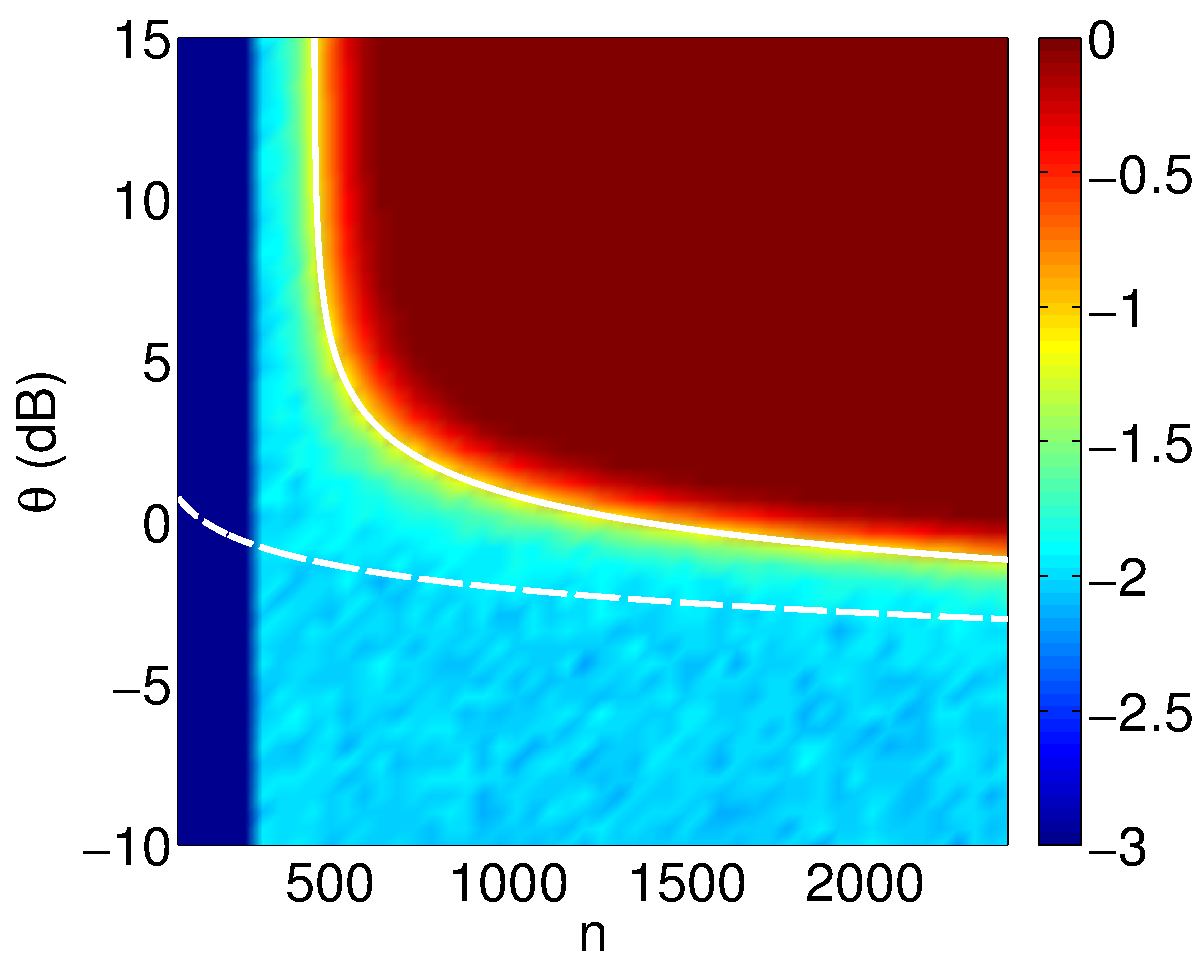
\includegraphics[width=0.47\textwidth]{chpt4_det_corr/figs/cca_rho7.pdf}
    }
    \subfigure[Empirical CCA $\rho=0.9$]{
      \label{fig:chpt4:cca_rho9}
      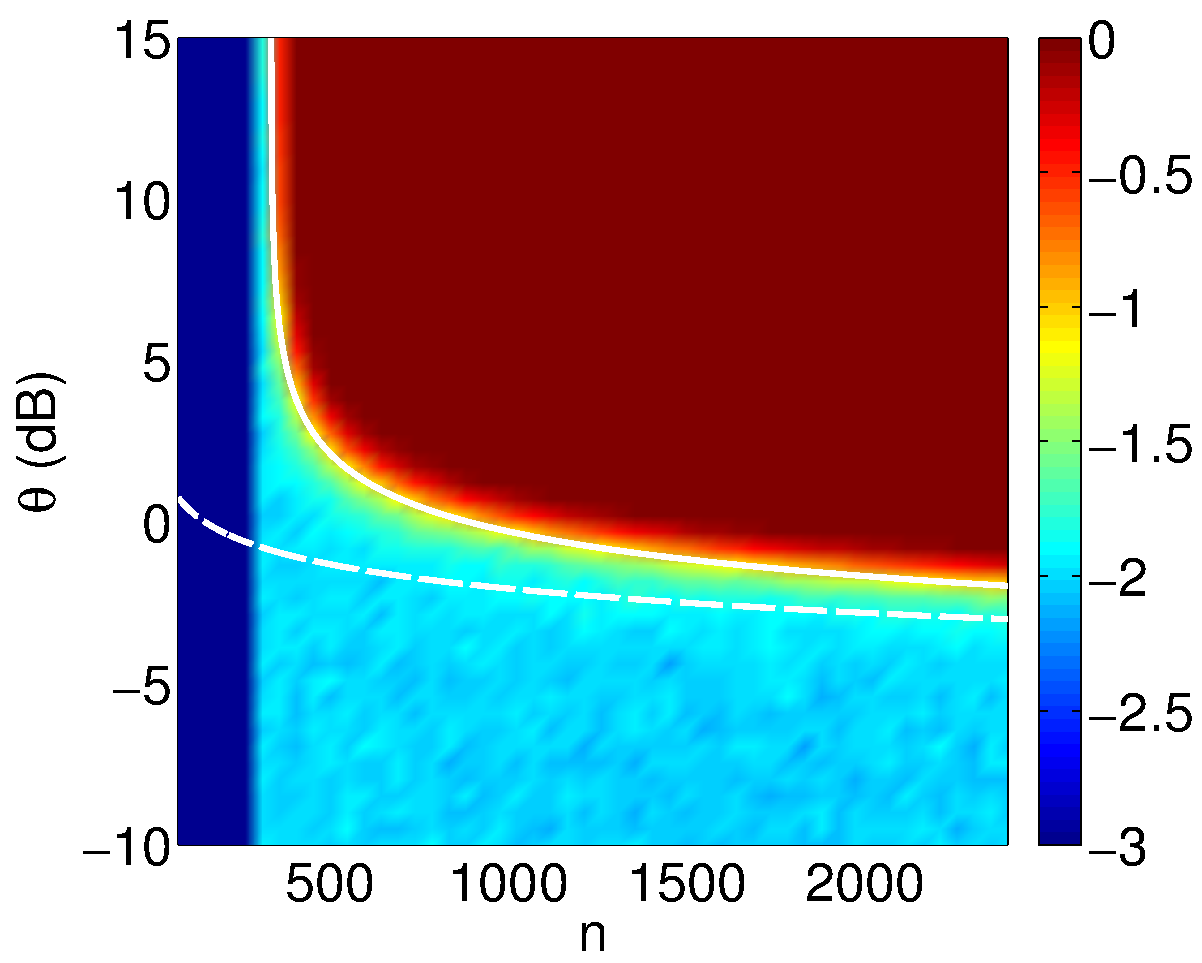
\includegraphics[width=0.47\textwidth]{chpt4_det_corr/figs/cca_rho9.pdf}
    }   
    \subfigure[ICCA $\rho=0.7$]{
      \label{fig:chpt4:icca_rho7}
      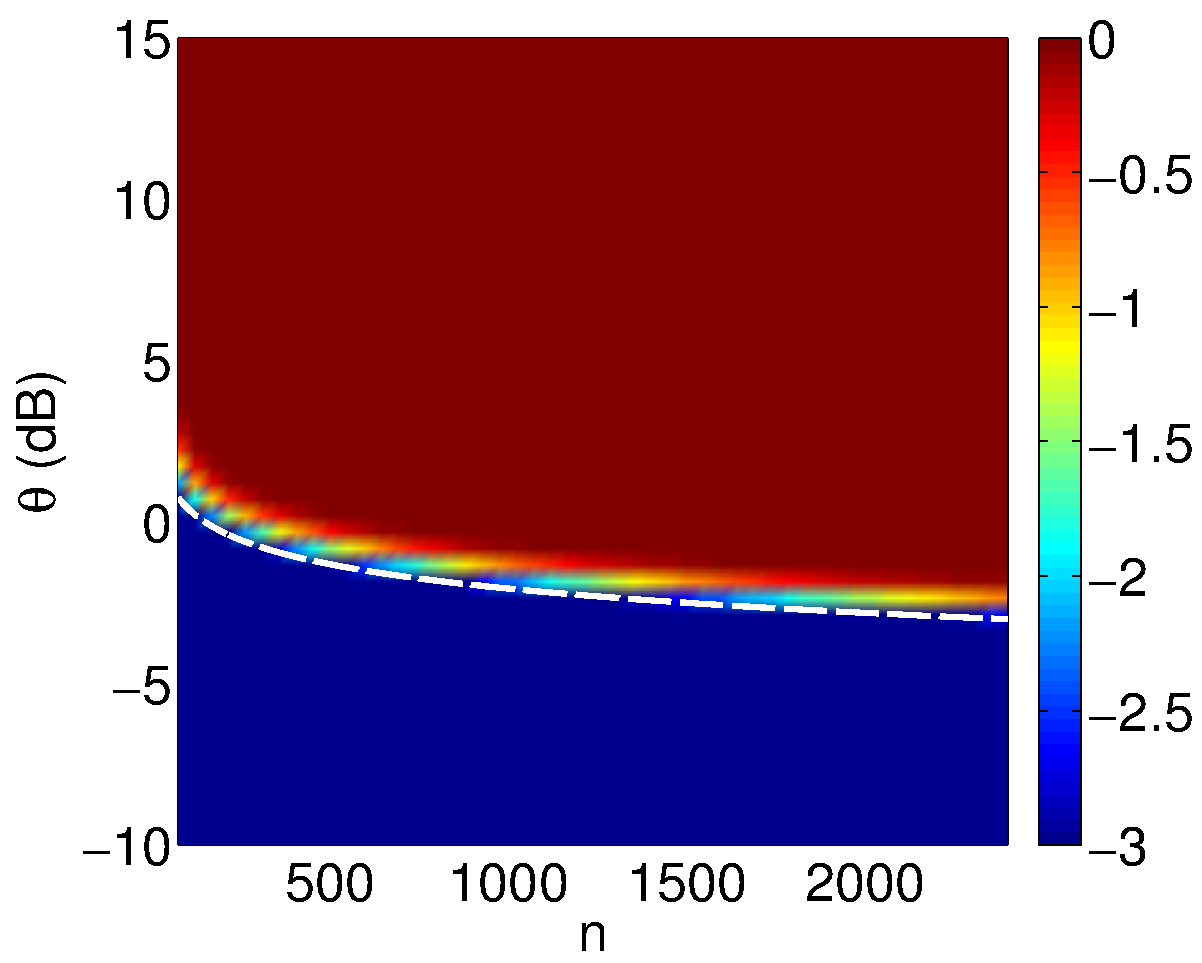
\includegraphics[width=0.47\textwidth]{chpt4_det_corr/figs/icca_rho7.pdf}
    }
    \subfigure[ICCA $\rho=0.9$]{
      \label{fig:chpt4:icca_rho9}
      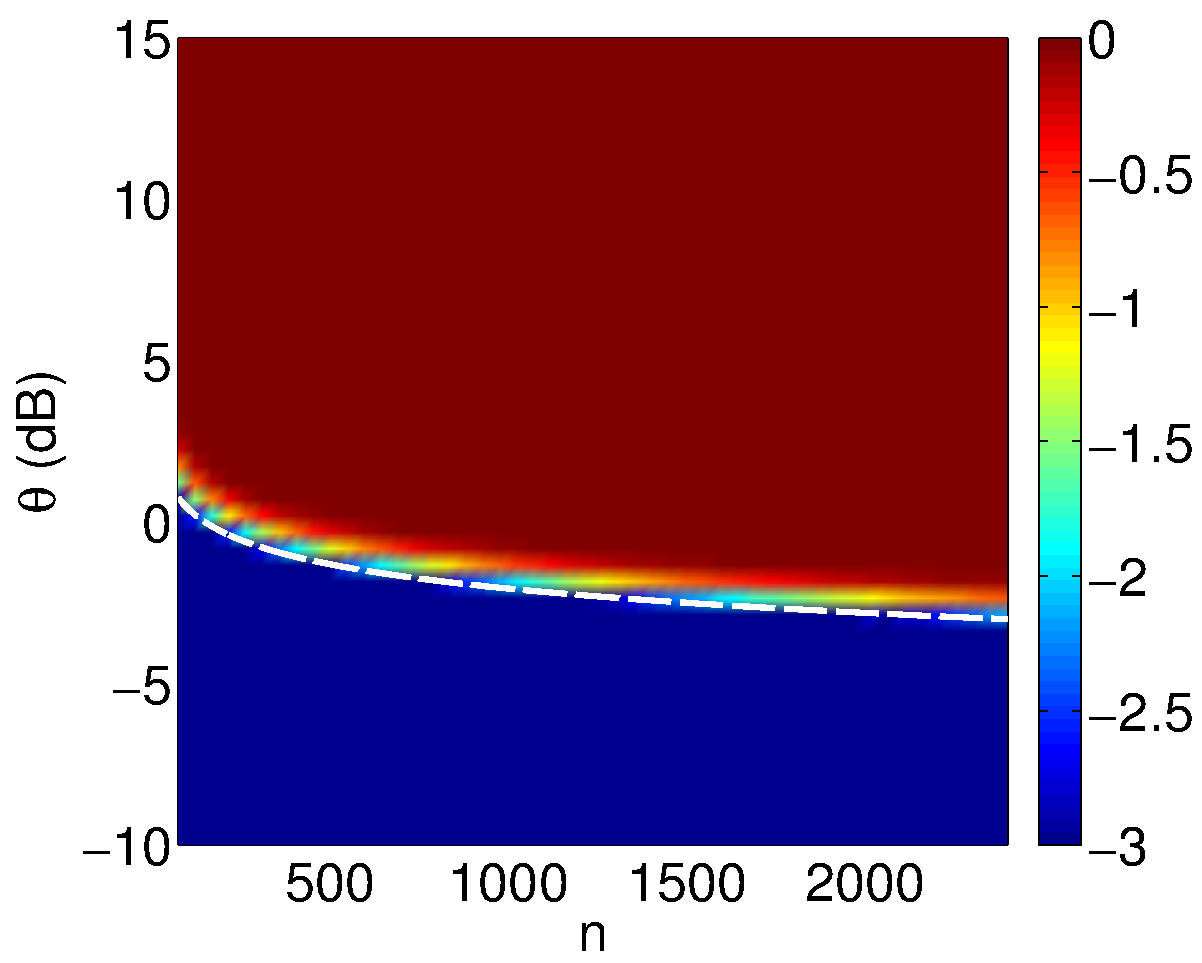
\includegraphics[width=0.47\textwidth]{chpt4_det_corr/figs/icca_rho9.pdf}
    }   
    \caption{We generate data from (\ref{eq:chpt4:data_model}) for $p=q=150$, $\kx=\ky=1$,
      $k=1$, and various $\rho=\Pxy$ and sweep over $\theta = \tx_1=\ty_1$ and $n$. We
      compute $\kxhat$ and $\kyhat$ as outlined in Appendix D for a significance value of
      $\alpha=0.01$. Using these estimates, we compute $\rhohatcca^{(1)}$ as the largest
      singular value of $\Cccahat$ as in (\ref{eq:chpt4:rhohatcca}) and
      $\rhohaticca^{(1)}$ as the largest singular value of $\Ciccahat$ as in
      (\ref{eq:chpt4:rhohaticca}). We then estimate the number of correlated signals
      $\khatcca$ and $\khaticca$ via (\ref{eq:chpt4:khats}) for a significance level of
      $\alpha=0.01$. We repeat this for 10000 trials and compute the percentage of trials
      where $\khatcca=1$ and $\khaticca=1$. We plot $\log_{10}$ of these percentages for
      multiples values of $\theta$ and $n$. We plot the theoretical consistency boundary
      of CCA (given in Theorem \ref{th:khat_lims} that relies on \cite{bao2014canonical})
      in a solid white line and the theoretical consistency boundary of ICCA (given in
      Theorem \ref{th:khat_lims}) in a dashed white line.}
    \label{fig:chpt4:cca_pt}
  \end{center}
\end{figure}

Next, we explore the minimum $1/c$ for $c=c_x=c_y$ needed to reliably detect $k=1$
correlated signal in the experiment setting described for Figure \ref{fig:chpt4:cca_pt}. As $c=p/n=q/n$, the minimum $1/c$ is equivalent to the minimum
number of samples needed for fixed dimensions. Using the theoretical phase transitions in
Theorem \ref{th:khat_lims}, we have that this critical value of $c$ is $c_{\text{crit}} =
\theta^4$ for ICCA and $c_{\text{crit}} =
\min\left(\frac{r_c^{\text{crit}}}{1+r_c^{\text{crit}}}, 0.5\right)$ for empirical CCA, where 
\be
r_c^{\text{crit}} = \left(\frac{-\rho +
    \sqrt{\rho^2+4\theta^2\rho^2(1+\theta^2\rho^2)}}{2(1+\theta^2\rho^2)}\right)^2.  
\ee
Figure \ref{fig:chpt4:contours} plots level sets of $c_{\text{crit}}$ for empirical CCA
and ICCA for various values of $\theta=\tx_1=\ty_1$ and $\rho=\Pxy$. Recall that if
$c>0.5$, empirical CCA fails entirely, so for comparison we only show contour lines for
$1/c=10$ and $1/c=3$.

From this figure, we once again observe that the performance of ICCA is independent of the
value of $\rho=\Pxy$, while the performance of empirical CCA is highly dependent on the
correlation. This figure allows us to showcase that ICCA is theoretically better than
empirical CCA in all parameter regimes as ICCA can achieve the same performance of
empirical CCA given fewer samples at a lower SNR.

\begin{figure}
  \begin{center}
    \subfigure[Empirical CCA]{
      \label{fig:chpt4:cca_contours}
      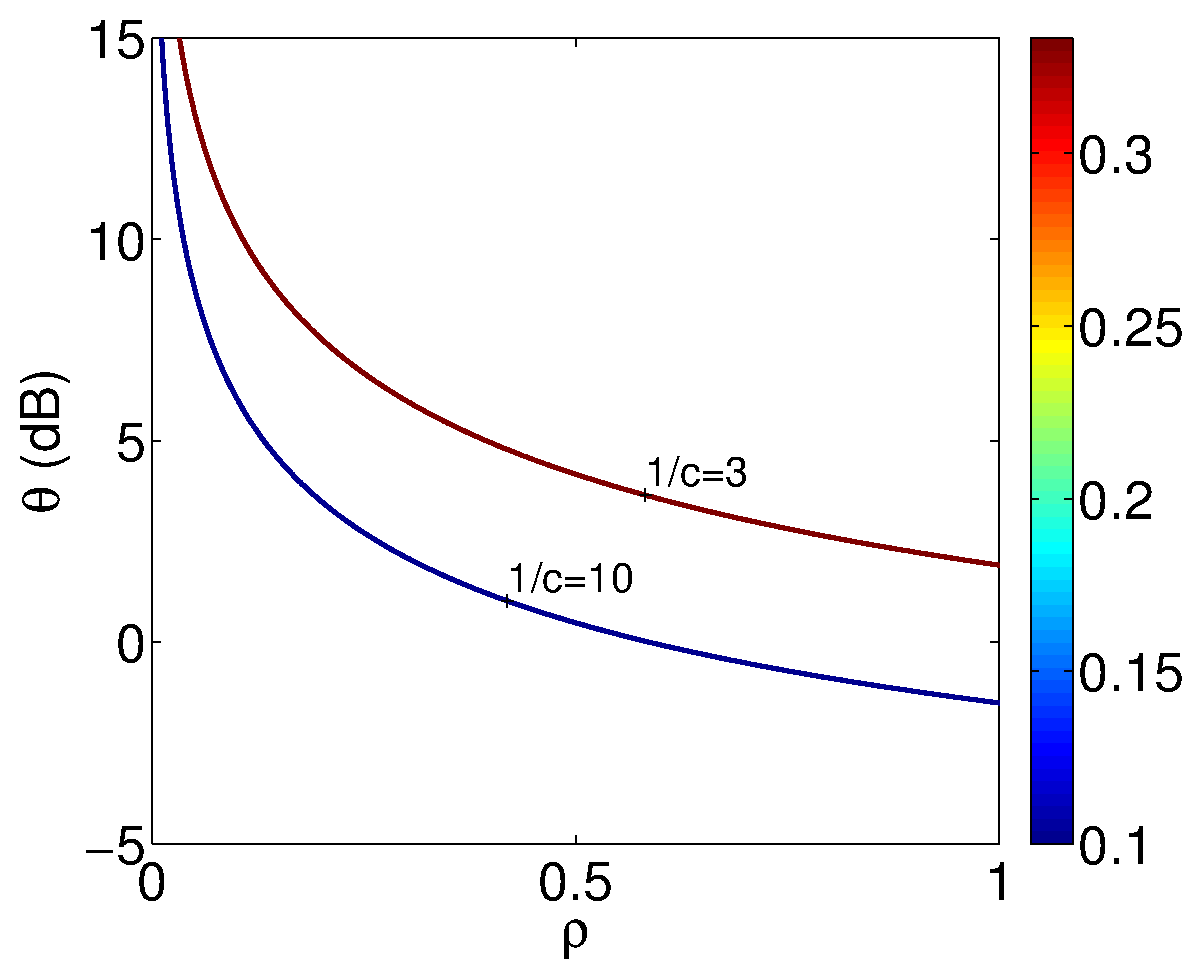
\includegraphics[width=0.47\textwidth]{chpt4_det_corr/figs/contours_cca.pdf}
    }
    \subfigure[ICCA]{
      \label{fig:chpt4:icca_contours}
      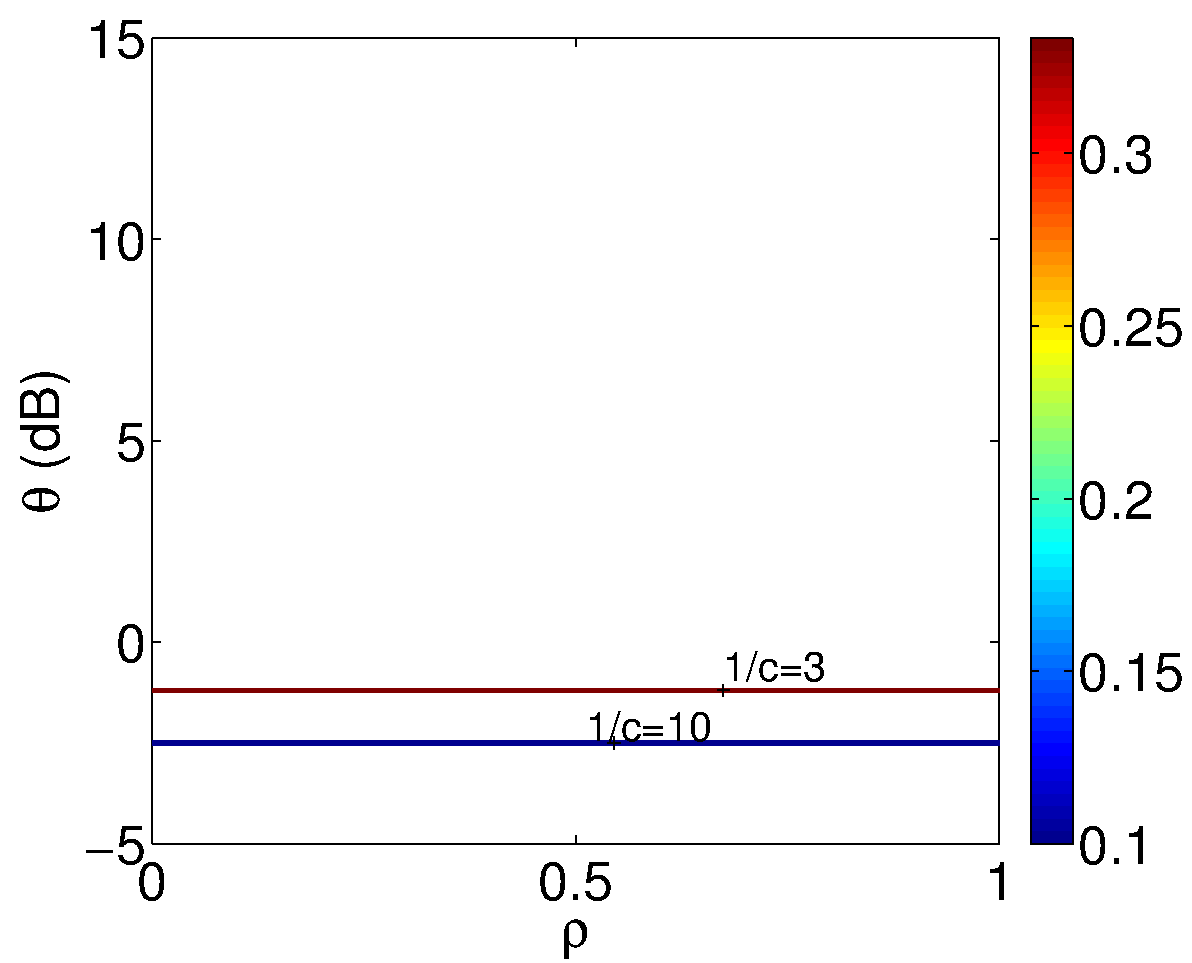
\includegraphics[width=0.47\textwidth]{chpt4_det_corr/figs/contours_icca.pdf}
    }   
    \caption{Contour lines for minimum $1/c$ necessary for reliable detection of $k=1$
      correlated component. The quantity $1/c = n/p$ is equivalent to the number of
      samples per dimension of data. Figure \ref{fig:chpt4:cca_contours} plots the
      contours for empirical CCA and Figure \ref{fig:chpt4:icca_contours} plots the ICCA
      contours using the limits give in Theorem \ref{th:khat_lims} for $c=c_x=c_y$. We
      plot the contours for $1/c=10$ to $1/c=3$.  These plots clearly demonstrate the ICCA
      limits are independent of $\rho=\Pxy$ while CCA is highly dependent on
      $\rho=\Pxy$. For a fixed number of samples (fixed $c$), ICCA is reliably detect the
      presence of a correlated signal at lower SNR values than empirical CCA.}
    \label{fig:chpt4:contours}
  \end{center}
\end{figure}

Finally, we show the detection ability of ICCA as a function of $\theta_x$ and $\theta_y$
for a rank-1 setting with $c_x=c_y=1$ in Figure \ref{fig:chpt4:theta_theta_heatmap}. This
figure succinctly summarizes Theorem \ref{th:khat_lims}. When either $\theta_x$ or
$\theta_y$ is less than the critical value of 1, we cannot reliably detect the presence of
correlation between the two datasets. This corresponds to the blue and green regions in
the figure. The blue region corresponds to when both SNRs are below the phase transition
and neither signal is detectable. The green region corresponds to when only one SNR is
above the phase transition; however, as the other SNR is below the phase transition, we
still cannot detect the presence of correlation. Only when both SNRs are above the phase
transition (yellow region) can we reliably detect the presence of correlation. Most
importantly, the regions in this figure are independent of the correlation between the two
datasets.

\begin{figure}
  \begin{center}
    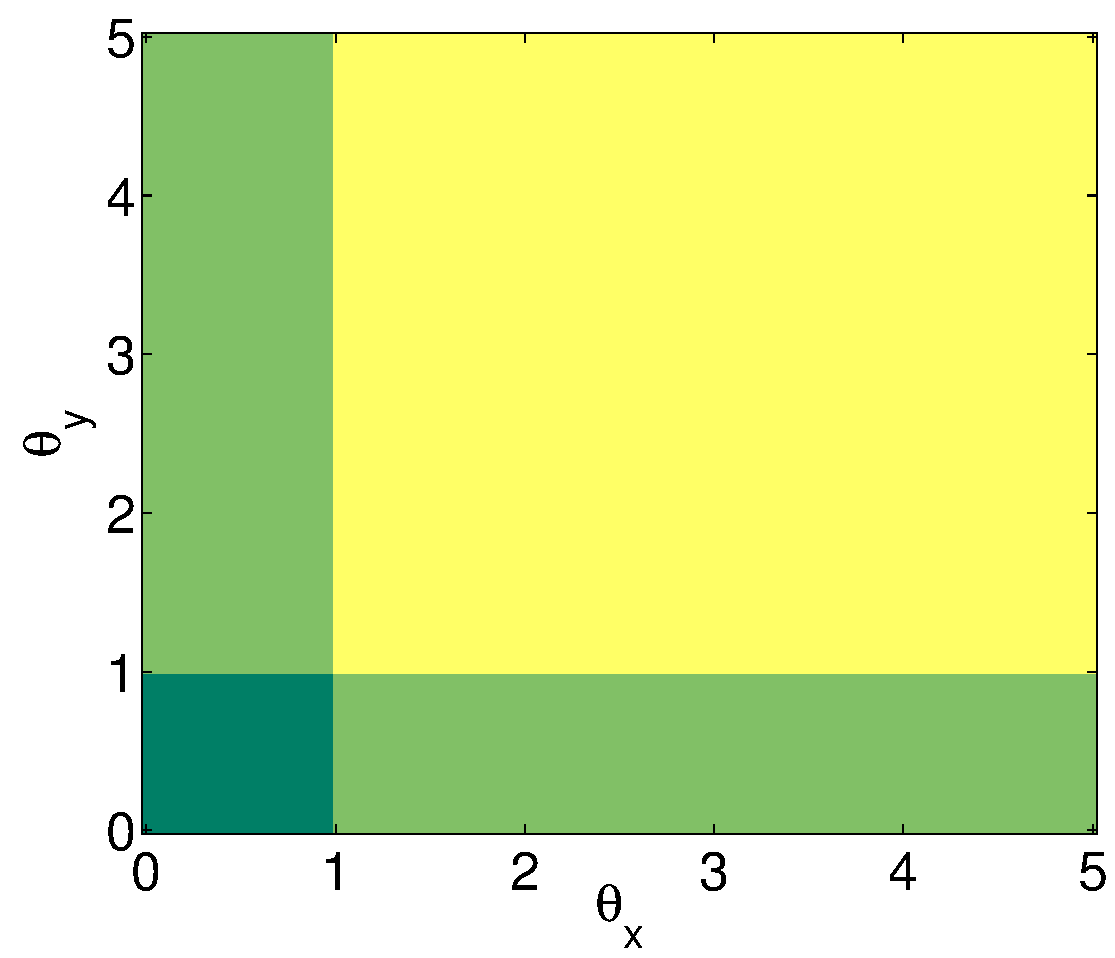
\includegraphics[width=0.47\textwidth]{chpt4_det_corr/figs/theta_theta_heatmap.pdf}
    \caption{Theoretical detection regions for ICCA for a rank-1 setting where
      $c_x=c_y=1$. In this setting, $\theta>1$ implies that the corresponding subspace is
      informative. Therefore, in light of Theorem \ref{th:khat_lims}, we see that when
      both $\theta_x<1$ and $\theta_y<1$, neither subspace component is informative and we
      cannot detect the presence of a correlated signal. This corresponds to the blue
      region. When only one of $\theta_x$ or $\theta_y$ is above the phase transition
      (green region), we still cannot detect the presence of a correlated signal even
      though we have one informative signal. However, when both $\theta_x$ and $\theta_y$
      are above the phase transition (yellow region), we can detect the presence of a
      correlated signal between the datasets. This detection ability is independent of the
      value of correlation between the datasets. }
    \label{fig:chpt4:theta_theta_heatmap}
  \end{center}
\end{figure}

\subsection{Comparison to Wilks Lambda Test}

Next we compare the classical Wilk's Lambda Test presented in Section
\ref{sec:chpt4:wilks} to the statistical tests developed in this section in
(\ref{eq:chpt4:khats}). We create two synthetic rank-1 signal-plus-noise data matrices of
dimension $p=150$ and $q=200$. We set the SNR of the signal in each dataset to
$\tx_1=\ty_1=2$ and the correlation between the signals to
$\rho=\Pxy=0.9$. For multiple value of $n$, we compute the correlations
returned by both ICCA and CCA. Using these correlations, we use our statistical tests in
(\ref{eq:chpt4:khats}) to determine whether the largest correlations, $\rhohatcca^{(1)}$
and $\rhohaticca^{(1)}$, are significant. Similarly we use the Wilk's test in
(\ref{eq:chpt4:wilks}) to determine for both CCA and ICCA whether the largest correlation
is significant. We note that for the Wilk's test, we need all $\min(p,q)$ correlations
returned by CCA and all $\min(\kx,\ky)$ correlations returned by ICCA. We repeat this
process for 250 trials for each values of $n$. Figure \ref{fig:chpt4_wilks} plots the
average percentage of trials where the correlation was significant for each statistical
test for each algorithm.

\begin{figure}
  \begin{center}
    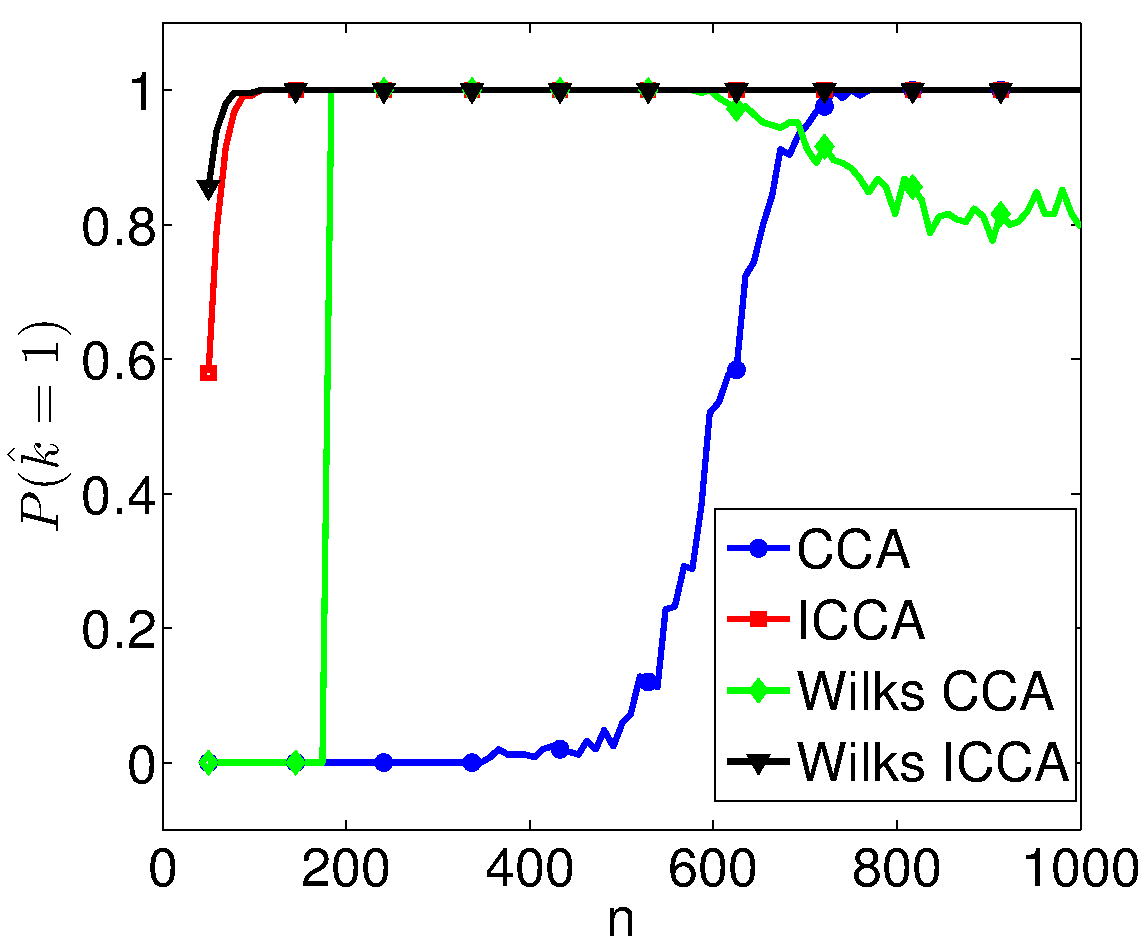
\includegraphics[width=0.6\textwidth]{chpt4_det_corr/figs/wilks_comp.pdf}
    \caption{We generate data from (\ref{eq:chpt4:data_model}) for $p=q=150$,
      $\kx=\ky=1$, $k=1$, $\tx_1=\ty_1=2$, $\Pxy=1$, and $\kxhat=\kyhat=1$. We compute
      $\rhohatcca^{(1)}$ as the largest singular value of $\Cccahat$ as in
      (\ref{eq:chpt4:rhohatcca}) and $\rhohaticca^{(1)}$ as the largest singular value of
      $\Ciccahat$ as in (\ref{eq:chpt4:rhohaticca}). We then estimate the number of
      correlated signals $\khatcca$ and $\khaticca$ using the Wilks test in
      (\ref{eq:chpt4:wilks}) and our new test in (\ref{eq:chpt4:khats}) for a significance
      level of $\alpha=0.01$. We repeat this for 250 trials and compute the percentage of
      trials where $\khatcca=1$ and $\khaticca=1$ for each significance test. We repeat
      this for multiple values of $n$ and plot the results. We observe that the classical
      Wilk's Lambda test is suboptimal and results in a large number of false alarms.}
    \label{fig:chpt4_wilks}
  \end{center}
\end{figure}

From this figure, we observe that the classical Wilk's Lambda test is suboptimal for
testing the presence of a correlation in the low-rank signal-plus-noise model for both
empirical CCA and ICCA. We know from our analysis in Theorem \ref{th:khat_lims} and the
empirical exploration on synthetic datasets from the previous section that the empirical
CCA and ICCA test statistics that we developed consistently estimate the presence of
correlated signals in low-rank signal-plus-noise datasets. Examining the performance of
the Wilk's test for determining the significance of the top ICCA correlation, we observe
that it predicts the presence of correlation before our consistent test
statistic. Therefore, using the Wilk's test statistic for ICCA will result in a high false
alarm rate. Similarly for empirical CCA, we see that the Wilk's test is very bad in the
sample-starved regime. Here our test statistic correctly predicts that the top empirical
CCA correlation is not significant because it is deterministically one. However, the
Wilk's test returns that the correlation is significant. Even worse, once we have enough
samples so that the top empirical CCA correlation is indeed significant, the Wilk's test
does not always predict a that the correlation is significant. Therefore, for empirical
CCA, the Wilk's test will have a large false-alarm rate in the low-sample regime and a
lower detection rate in the moderate-sample regime. The classical Wilk's test is
suboptimal for determining the significance of correlations of both empirical CCA and ICCA
and we encourage practitioners to instead use our consistent test statistics.

\subsection{Simulated Missing Data}

Next, we demonstrate the accuracy of the consistency bound for both empirical CCA and ICCA
in the setting of missing data described in Theorem \ref{th:missing_data}. Again, we
consider a rank-1 setting ($\kx=\ky=1$) but generate data from
(\ref{eq:chpt4:data_model_miss}) for fixed $p=q=150$ over various number of samples $n$,
signal-to-noise ratio (SNR) $\theta=\tx_1=\ty_1$, various $\rho=\Pxy$ (so that $k=1$), and
also various percentages of missing data $\gamma=\gamma_x=\gamma_y$. In all simulations,
we use Algorithm 2 of \cite{nadakuditi2010fundamental} to estimate $\kxhat$ and $\kyhat$
using a significance level of $\alpha=0.01$. We stack the data into matrices $X$ and $Y$,
and compute $\rhohatcca^{(1)}$ and $\rhohaticca^{(1)}$ from the SVD of of $\Cccahat$ and
$\Ciccahat$, respectively. Using these correlation estimates, we compute the estimated
number of correlated components via (\ref{eq:chpt4:khats}) for a significance level of
$\alpha=0.01$. For a fixed set of parameters ($n$, $\theta$, $\rho$, $\gamma$) we repeat
the above process for 10000 trials and determine the percentage of trials where we detect
$\khatcca=1$ and $\khaticca=1$. Figure \ref{fig:chpt4:cca_missing_75} plots the
$\log_{10}$ of this percentage for empirical CCA and ICCA, respectively. On each plot, we
overlay the consistency boundary given by Theorem \ref{th:missing_data}.

From these figures, we observe that Theorem \ref{th:missing_data} accurately predicts the
phase transition for both empirical CCA and ICCA in the presence of missing data for a
wide array of parameters. When $n<p+q$ empirical CCA is unable to detect the correlated
signal while ICCA can reliably detect the correlated signal, even in the presence of
missing data. In this missing data setting, we once again observe that the value of $\rho$
affects the phase transition for empirical CCA but not for ICCA; it is harder for
empirical CCA to detect signals with small correlations.

\begin{figure}
  \begin{center}
    \subfigure[Empirical CCA $\rho=0.7$]{
      \label{fig:chpt4:cca_rho3_75}
      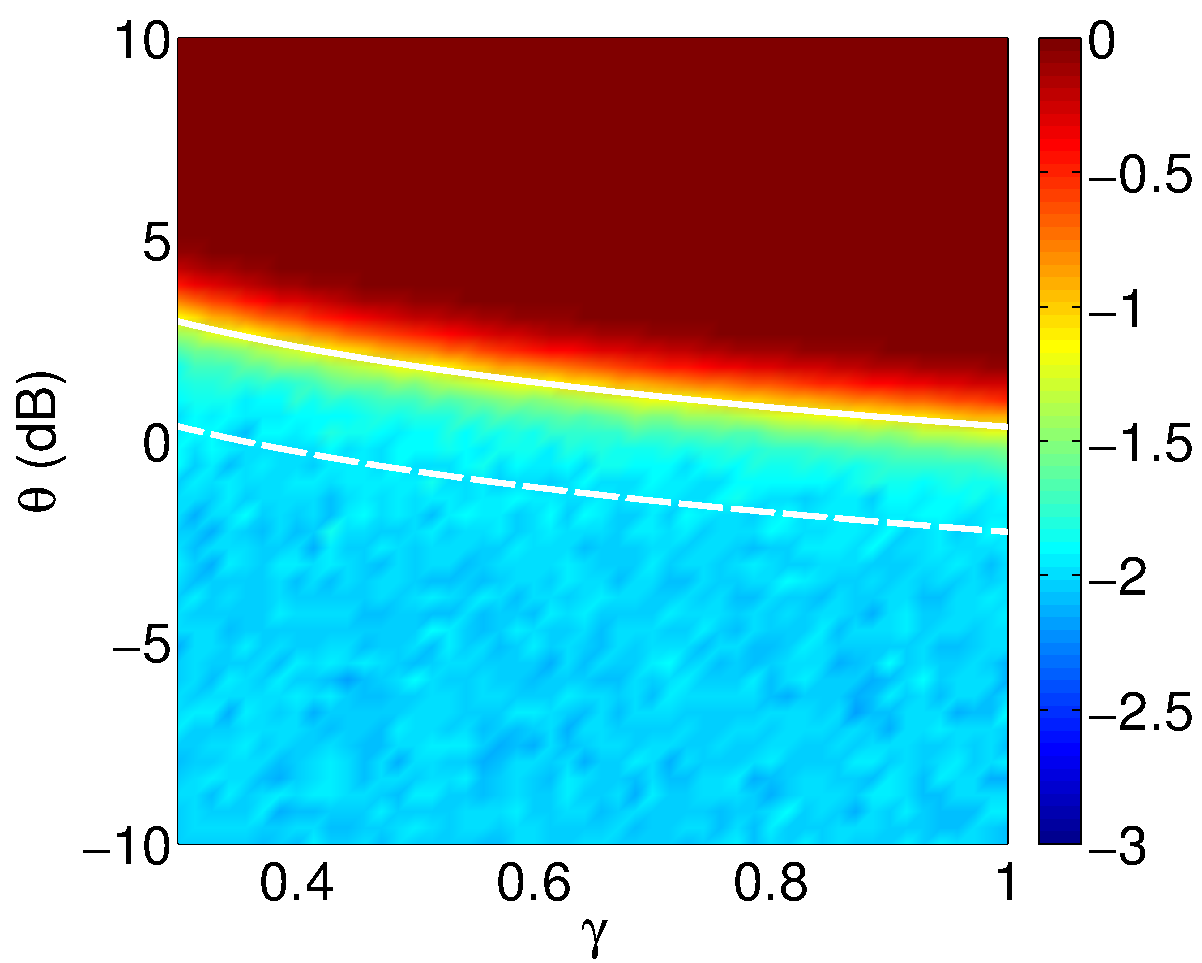
\includegraphics[width=0.47\textwidth]{chpt4_det_corr/figs/cca_missing_7_1200.pdf}
    }
    \subfigure[Empirical $\rho=0.9$]{
      \label{fig:chpt4:cca_rho5_75}
      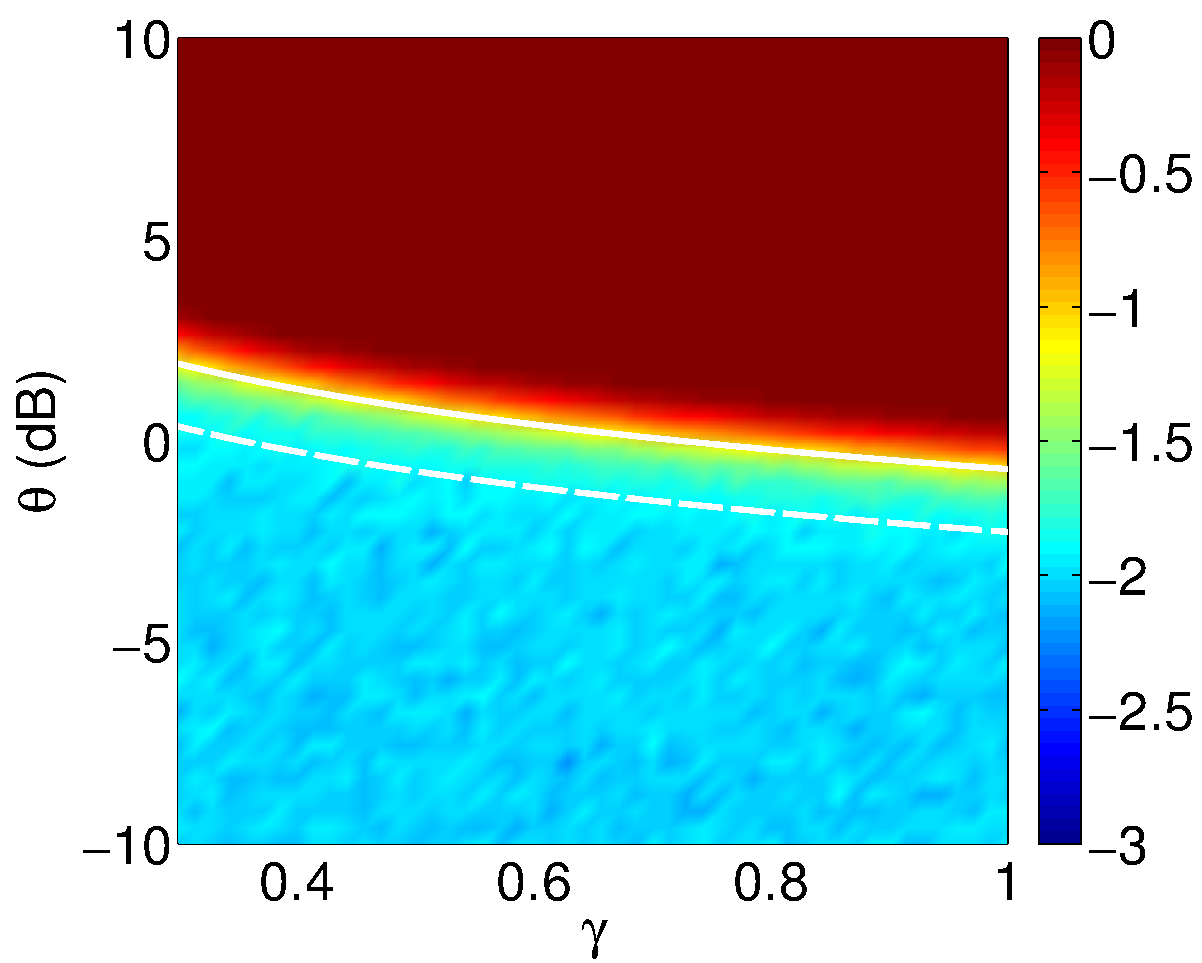
\includegraphics[width=0.47\textwidth]{chpt4_det_corr/figs/cca_missing_9_1200.pdf}
    }
    \subfigure[ICCA $\rho=0.7$]{
      \label{fig:chpt4:cca_rho7_75}
      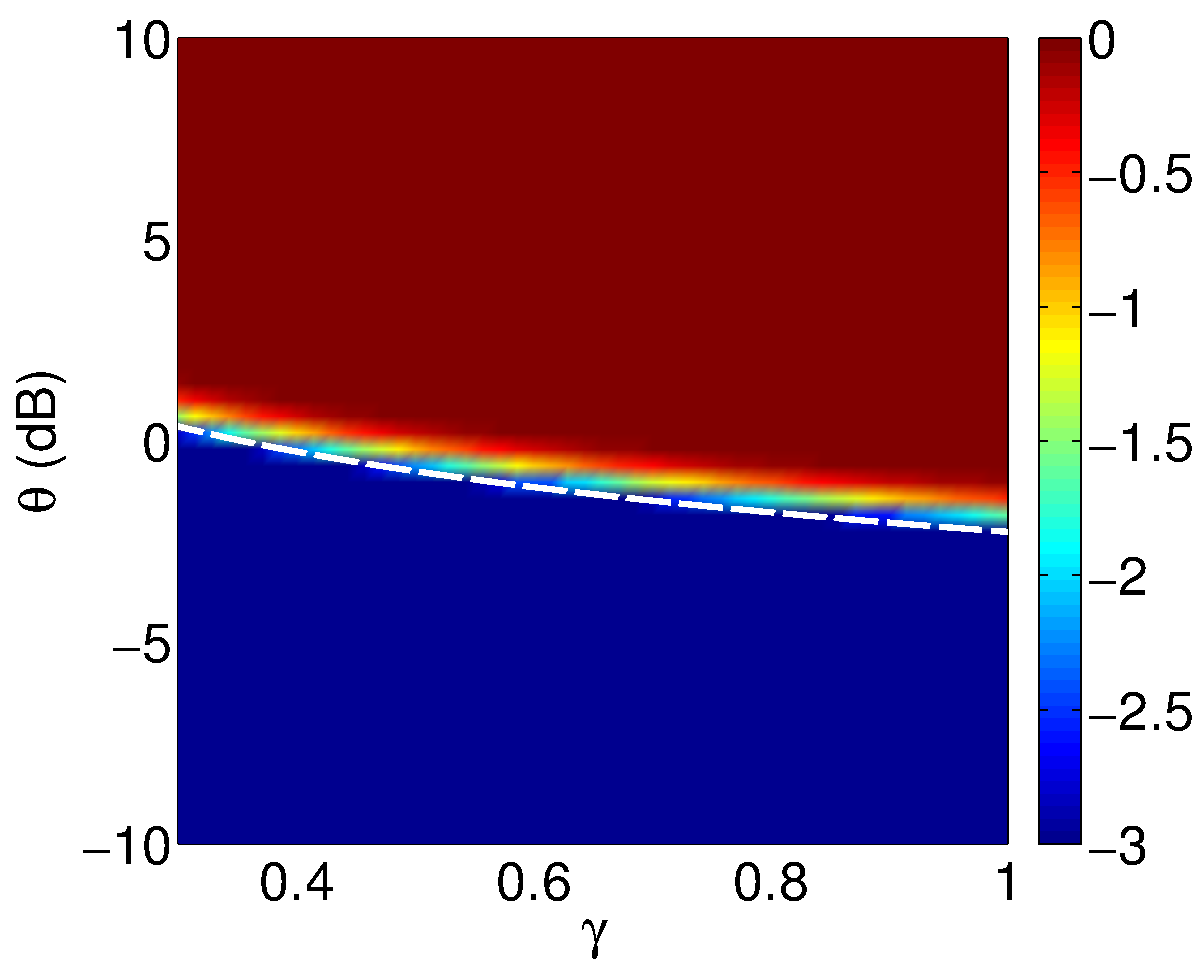
\includegraphics[width=0.47\textwidth]{chpt4_det_corr/figs/icca_missing_7_1200.pdf}
    }
    \subfigure[ICCA $\rho=0.9$]{
      \label{fig:chpt4:cca_rho9_75}
      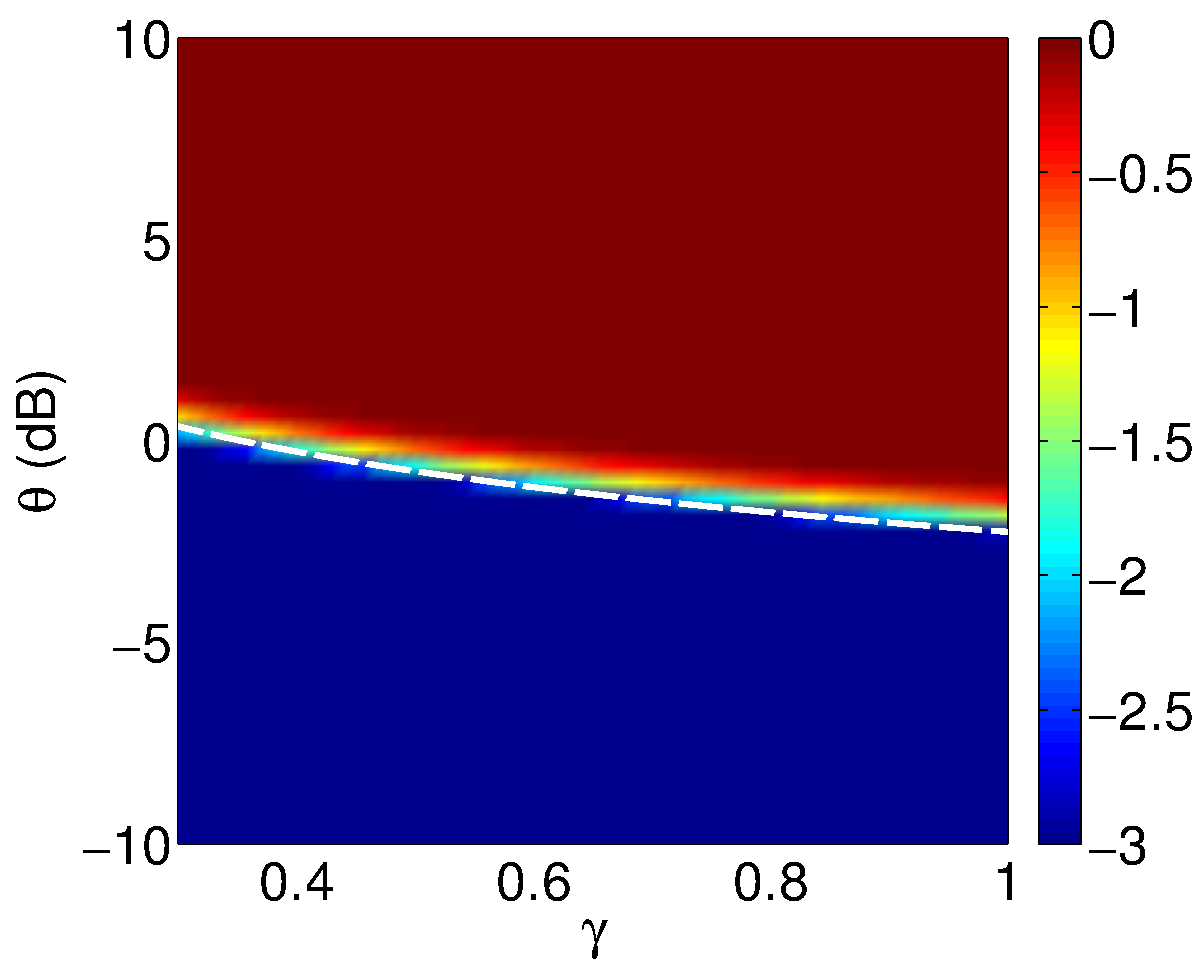
\includegraphics[width=0.47\textwidth]{chpt4_det_corr/figs/icca_missing_9_1200.pdf}
    }   
    \caption{We generate data from (\ref{eq:chpt4:data_model_miss}) for $p=q=150$,
      $\kx=\ky=1$, $k=1$, $n=1200$, and various $\rho=\Pxy$ and sweep over $\theta =
      \tx_1=\ty_1$ and $\gamma=\gamma_x=\gamma_y$. We compute $\kxhat$ and $\kyhat$ as
      outline in Appendix D for a significance value of $\alpha=0.01$. Using these
      estimates, we compute $\rhohatcca^{(1)}$ as the largest singular value of $\Cccahat$
      as in (\ref{eq:chpt4:rhohatcca}) and $\rhohaticca^{(1)}$ as the largest singular
      value of $\Ciccahat$ as in (\ref{eq:chpt4:rhohaticca}). We then estimate the number
      of correlated signals $\khatcca$ and $\khaticca$ via (\ref{eq:chpt4:khats}) for a
      significance level of $\alpha=0.01$. We repeat this for 10000 trials and compute the
      percentage of trials where $\khatcca=1$ and $\khaticca=1$. We plot $\log_{10}$ of
      these percentages for multiples values of $\theta$ and $n$. We plot the theoretical
      consistency boundary of empirical CCA (given in Theorem \ref{th:missing_data}) in a
      solid white line and the theoretical consistency boundary of ICCA (given in Theorem
      \ref{th:missing_data}) in a dashed white line.}
    \label{fig:chpt4:cca_missing_75}
  \end{center}
\end{figure}

\subsection{Controlled Flashing Lights Experiment}

To verify the effectiveness of ICCA for real world applications, we conducted a controlled
experiment consisting of 5 stationary flashing lights and two stationary iPhone
cameras. Figure \ref{fig:chpt4:flashing_sources} shows the left and right camera views at
one time point of our experiment and manually identifies each source. The 5 sources are a
blue flashing police light (BPL) outlined in the green rectangle, one phone with a
flashing strobe light (PH1) outlined in the dark blue rectangle, another phone with a
flashing strobe light (PH2) outlined in a red rectangle, a tablet with a flashing screen
(T1) outlined in the magenta rectangle, and a red flashing police light (RPL) outlined in
the cyan rectangle. From left to right, the left camera can see BPL, PH1, and PH2. From
left to right, the right camera can see PH2, T1, and RPL. Therefore, both cameras share
the common signal of PH2.

\begin{figure}
  \begin{center}
    \subfigure[Left Camera]{
      \label{fig:chpt4:flashing_left}
      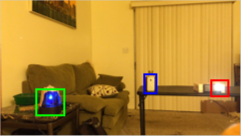
\includegraphics[width=0.47\textwidth]{chpt4_det_corr/figs/flashing_left_sources.png}
    }
    \subfigure[Right Camera]{
      \label{fig:chpt4:flashing_right}
      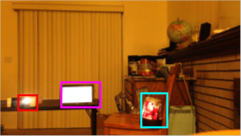
\includegraphics[width=0.47\textwidth]{chpt4_det_corr/figs/flashing_right_sources.png}
    }   
    \caption{Left and right camera views of our experiment with boxes manually identifying
      each source. Both cameras share a common flashing phone, outlined in a red
      rectangle. Each camera has two independent sources besides the shared flashing
      phone.}
    \label{fig:chpt4:flashing_sources}
  \end{center}
\end{figure}


To synchronize the cameras we used the RecoLive MultiCam iPhone app
\footnote{http://recolive.com/en/}. After turning on all light sources, we recorded
30 seconds of video at 30 frames per second. The resolutions of the iPhone's cameras were
both $1920\times 1080$ pixels. 

To post-process the video data, we first converted the video streams to grayscale and then
downsampled each spatial dimension by a factor of 8, resulting in a resolution of $240\times
135$. We then vectorized each image and stacked the 900 frames into data matrices, both
of dimension $32400 \times 900$. Finally, we subtract the mean from each dataset so that
we may run PCA, empirical CCA, and ICCA on the zero-mean datasets, $X_{\text{left}}$ and
$Y_{\text{right}}$.

First, we run PCA on $X_{\text{left}}$ and $Y_{\text{right}}$ to identify the number of
signals in each dataset. We know from our setup that each camera has 3
independent sources. Figure \ref{fig:chpt4:flashing_svs} plots the singular values of
$X_{\text{left}}$ and $Y_{\text{right}}$. Figures \ref{fig:chpt4:flashing_UL} and
\ref{fig:chpt4:flashing_UR} plot the singular vector heatmaps corresponding to the top 3
singular values of $X_{\text{left}}$ and $Y_{\text{right}}$, respectively. Each figure
also overlays a thresholded version of the singular vectors onto the raw video. The
threshold that we use is $\sqrt{\log(n)/n}$. From these figures, PCA does a good job at
identifying the pixels containing a signal (flashing light). 

\begin{figure}
  \begin{center}
    \subfigure[Left camera]{
      \label{fig:chpt4:lsv}
      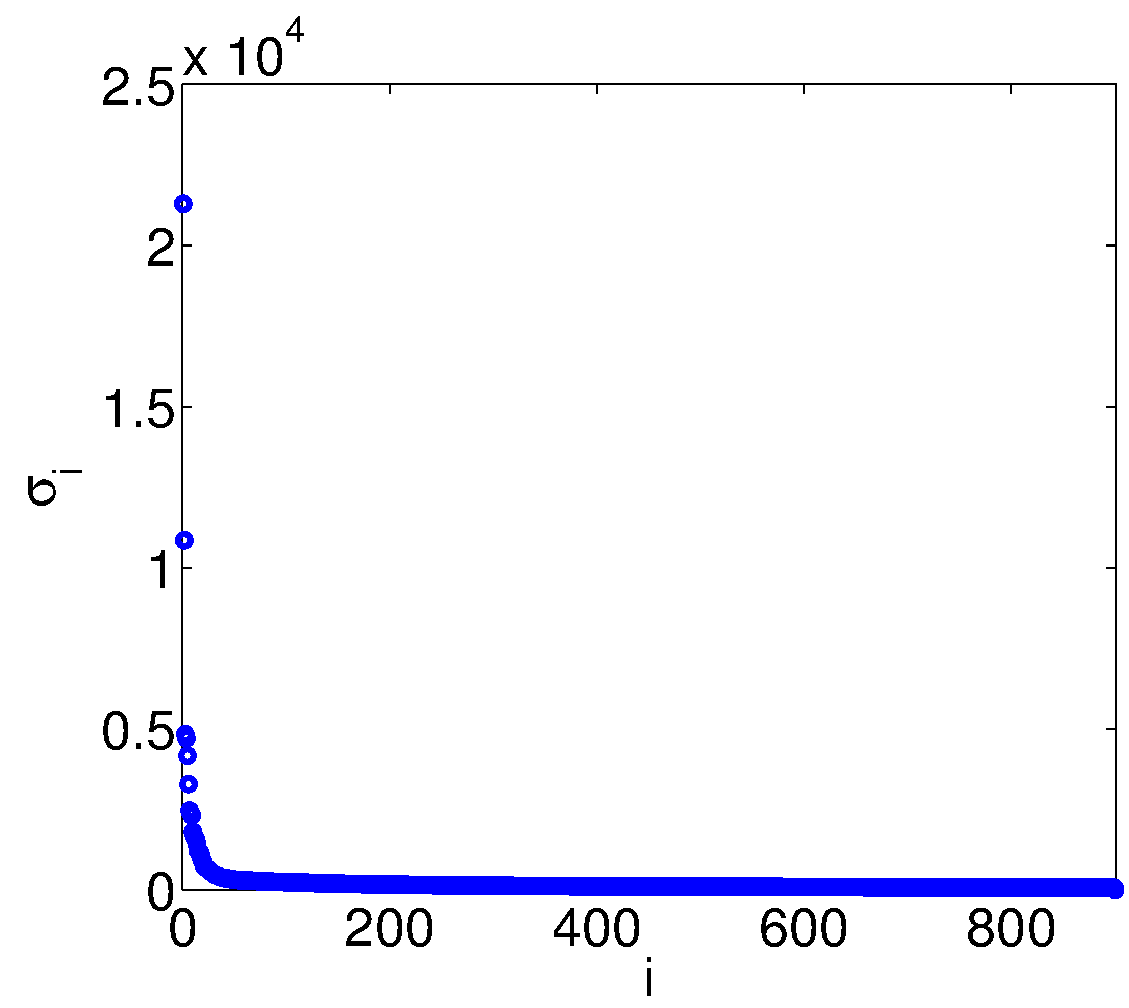
\includegraphics[width=0.47\textwidth]{chpt4_det_corr/figs/flashing_lsv.pdf}
    }
    \subfigure[Right camera]{
      \label{fig:chpt4:rsv}
      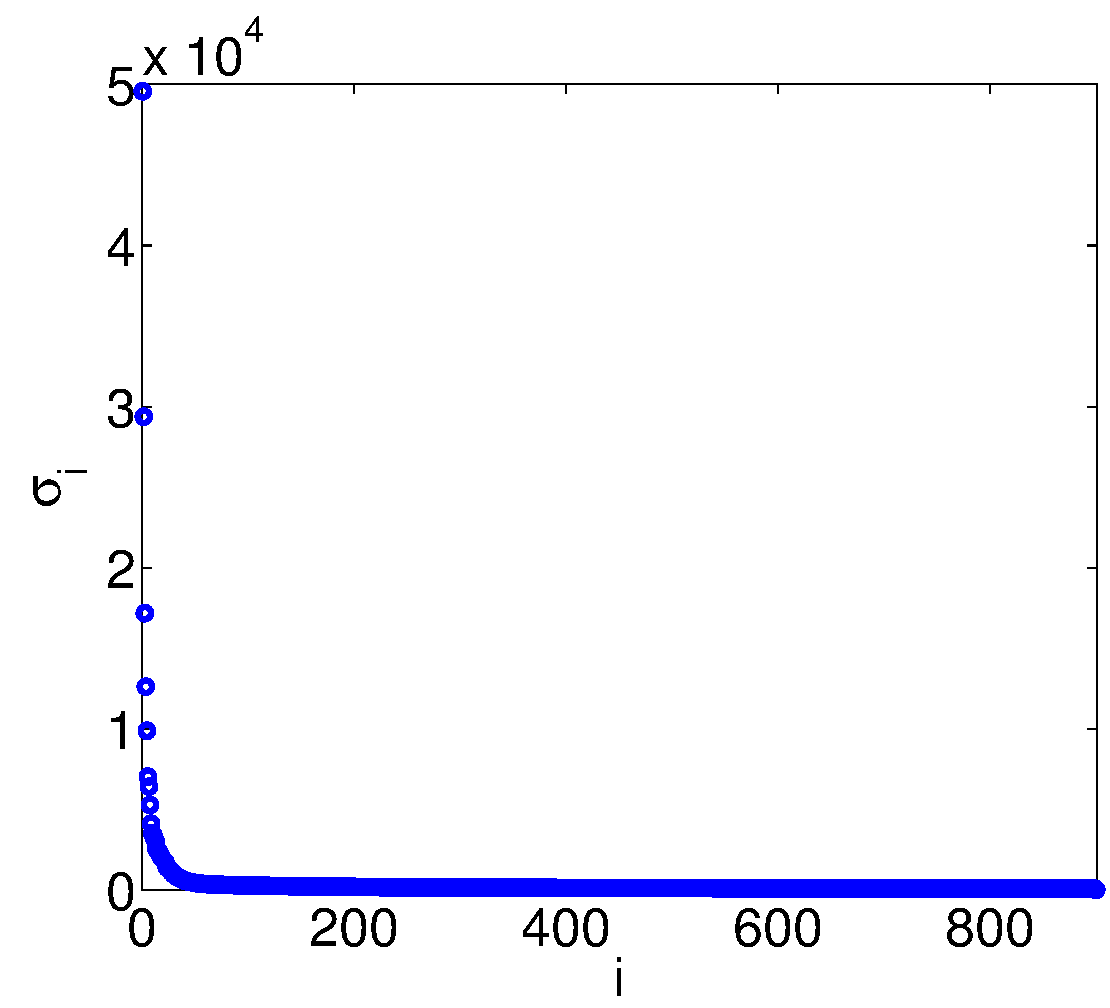
\includegraphics[width=0.47\textwidth]{chpt4_det_corr/figs/flashing_rsv.pdf}
    }   
    \caption{Singular value spectra of $X_{\text{left}}$ and $Y_{\text{right}}$ for the
      flashing light experiment.}
    \label{fig:chpt4:flashing_svs}
  \end{center}
\end{figure}

\begin{figure}
  \begin{center}
    \subfigure[$u_1$]{
      \label{fig:chpt4:ul1}
      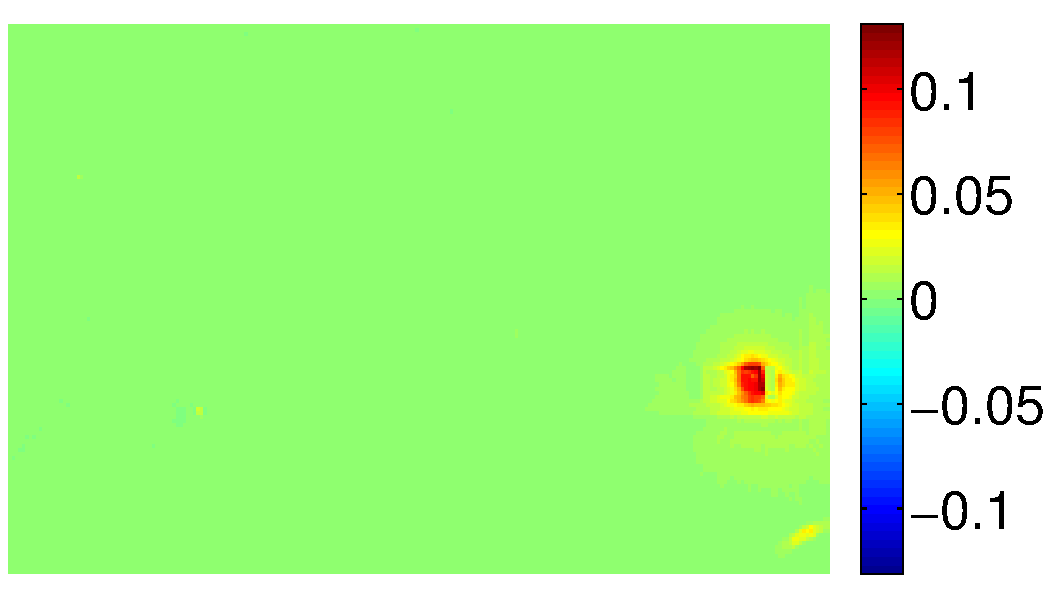
\includegraphics[width=0.47\textwidth]{chpt4_det_corr/figs/flashing_ul1.pdf}
    }
    \subfigure[$u_2$]{
      \label{fig:chpt4:ul2}
      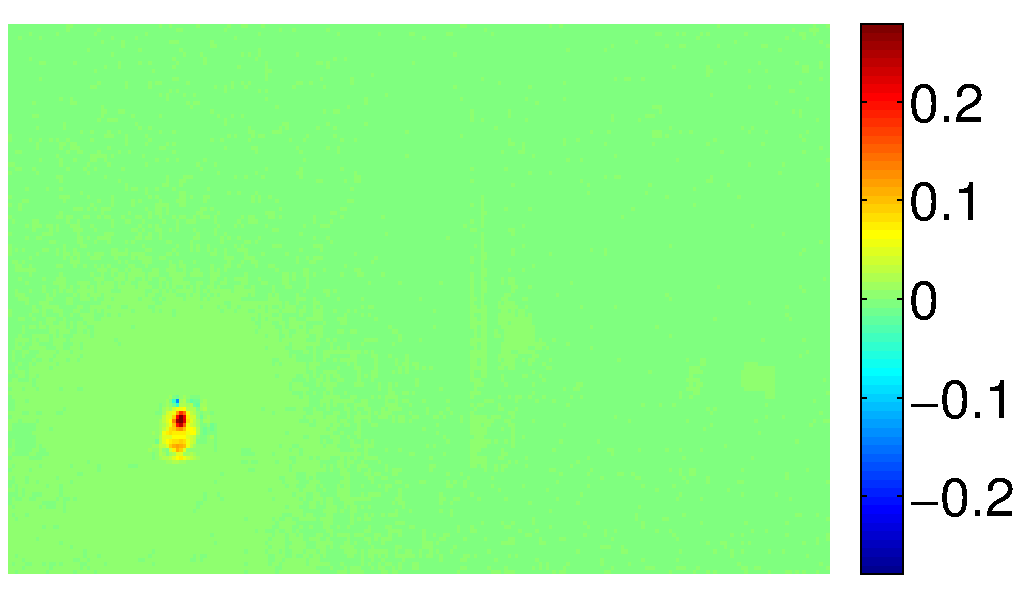
\includegraphics[width=0.47\textwidth]{chpt4_det_corr/figs/flashing_ul2.pdf}
    }   
    \subfigure[$u_3$]{
      \label{fig:chpt4:ul3}
      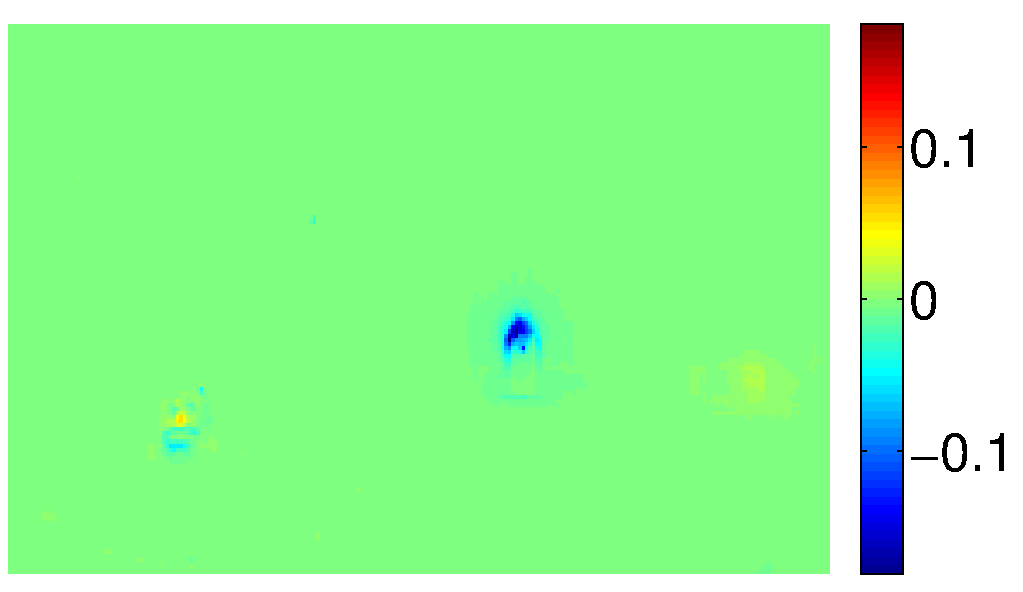
\includegraphics[width=0.47\textwidth]{chpt4_det_corr/figs/flashing_ul3.pdf}
    }
    \subfigure[Overlay]{
      \label{fig:chpt4:ul_overlay}
      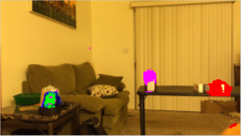
\includegraphics[width=0.47\textwidth]{chpt4_det_corr/figs/flashing_left_pca.png}
    }   
    \caption{(a)-(c) Left singular vectors of $X_{\text{left}}$ corresponding to the top 3
      singular values in Figure \ref{fig:chpt4:lsv}. (d) Thresholded singular vectors from
      (a)-(c) overlayed onto original scene. We use a threshold of $\log(p)/\sqrt{p}$
      where $p=32400$ pixels. These correspond to the 3 light sources visible in the left
      camera.The green pixels identify BPL; the magenta pixels identify PH1; the red
      pixels identify PH2.}
    \label{fig:chpt4:flashing_UL}
  \end{center}
\end{figure}

\begin{figure}
  \begin{center}
    \subfigure[$u_1$]{
      \label{fig:chpt4:ur1}
      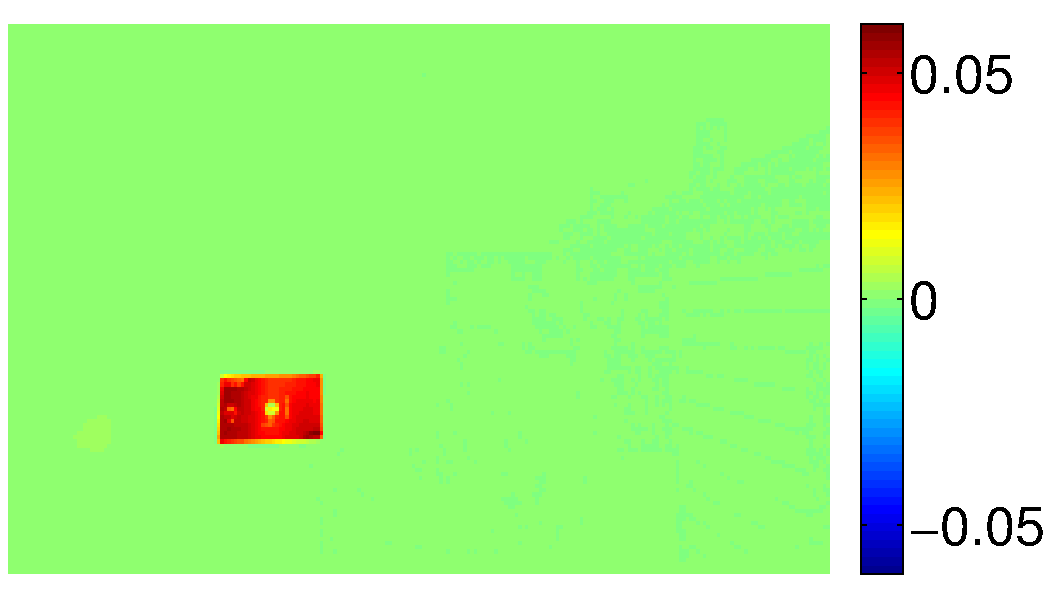
\includegraphics[width=0.47\textwidth]{chpt4_det_corr/figs/flashing_ur1.pdf}
    }
    \subfigure[$u_2$]{
      \label{fig:chpt4:ur2}
      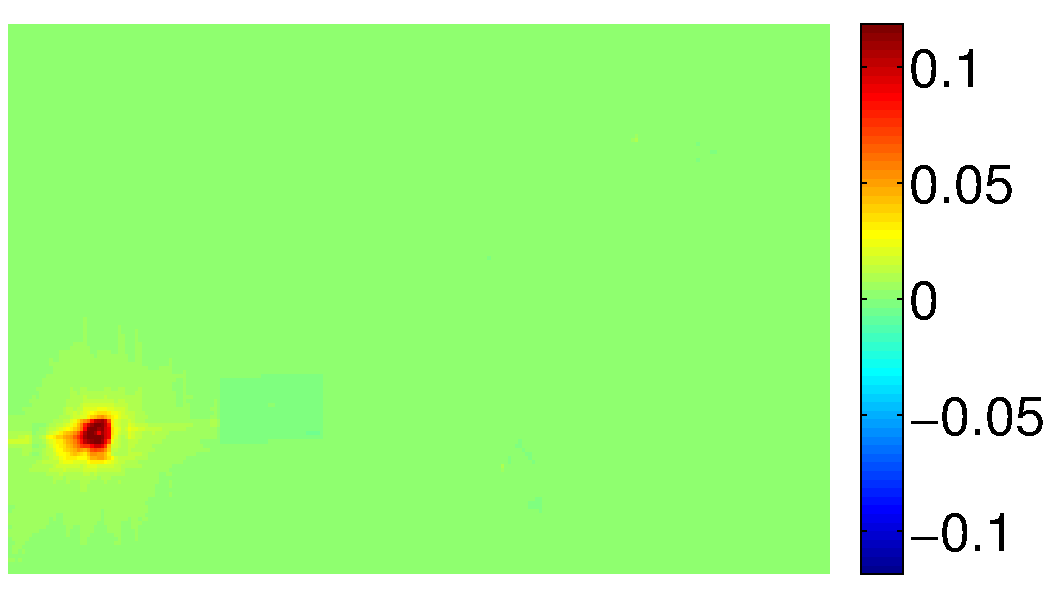
\includegraphics[width=0.47\textwidth]{chpt4_det_corr/figs/flashing_ur2.pdf}
    }   
    \subfigure[$u_3$]{
      \label{fig:chpt4:ur3}
      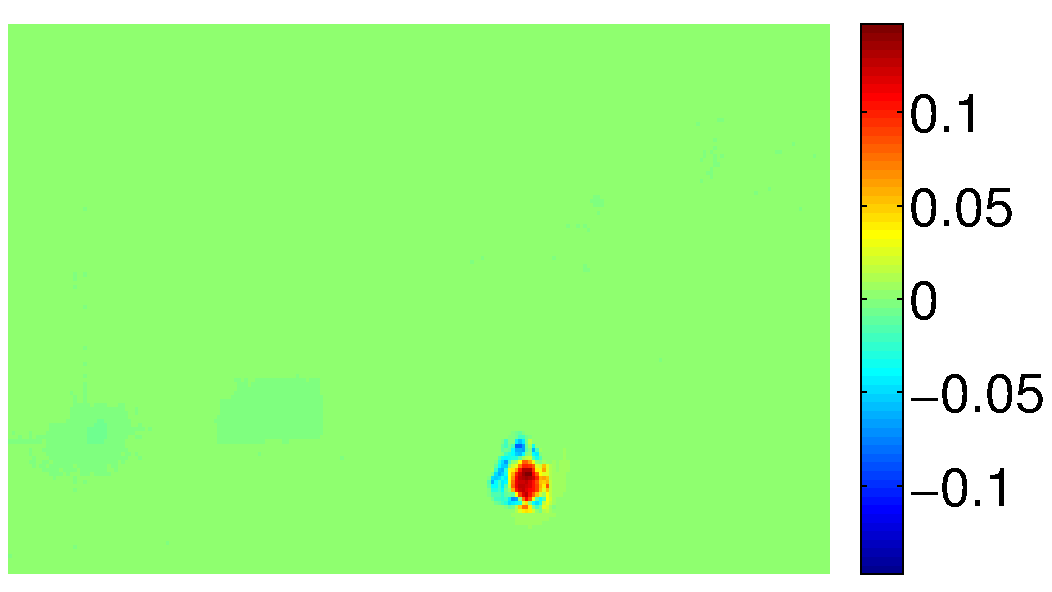
\includegraphics[width=0.47\textwidth]{chpt4_det_corr/figs/flashing_ur3.pdf}
    }
    \subfigure[Overlay]{
      \label{fig:chpt4:ur_overlay}
      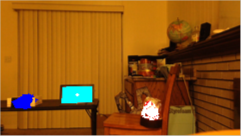
\includegraphics[width=0.47\textwidth]{chpt4_det_corr/figs/flashing_right_pca.png}
    }   
    \caption{(a)-(c) Left singular vectors of $Y_{\text{right}}$ corresponding to the top
      3 singular values in Figure \ref{fig:chpt4:rsv}. (d) Thresholded singular vectors
      from (a)-(c) overlayed onto original scene. We use a threshold of $\log(p)/\sqrt{p}$
      where $p=32400$ pixels. These correspond to the 3 light sources visible in the right
      camera. The dark blue pixels identify PH2; the cyan pixels identify T1; the white
      pixels identify RPL.}
    \label{fig:chpt4:flashing_UR}
  \end{center}
\end{figure}

However, PCA does not provided any information about whether the identified signals are
correlated across cameras. To identify correlated pixels between the cameras, we run
empirical CCA and ICCA after each new video frame. For frame $\ell$, we construct the
$32400\times\ell$ submatrices $X_{\text{left}}^\ell$ and $Y_{\text{right}}^\ell$ by taking
the matrix of the first $\ell$ original vectorized frames and zero meaning it. We then use
these matrices as the input to empirical CCA and ICCA. Using our knowledge of 3 sources
present in each camera, we set $\kxhat=\kyhat=3$. Figure \ref{fig:chpt4:flashing_corrs}
plots the top 3 correlation coefficients returned by empirical CCA and ICCA over the first
800 frames. Intuitively, empirical CCA returns perfect correlation as we have only a few
frames but a large dimension (pixels).

\begin{figure}
  \begin{center}
    \subfigure[CCA]{
      \label{fig:chpt4:flashing_cca_corrs}
      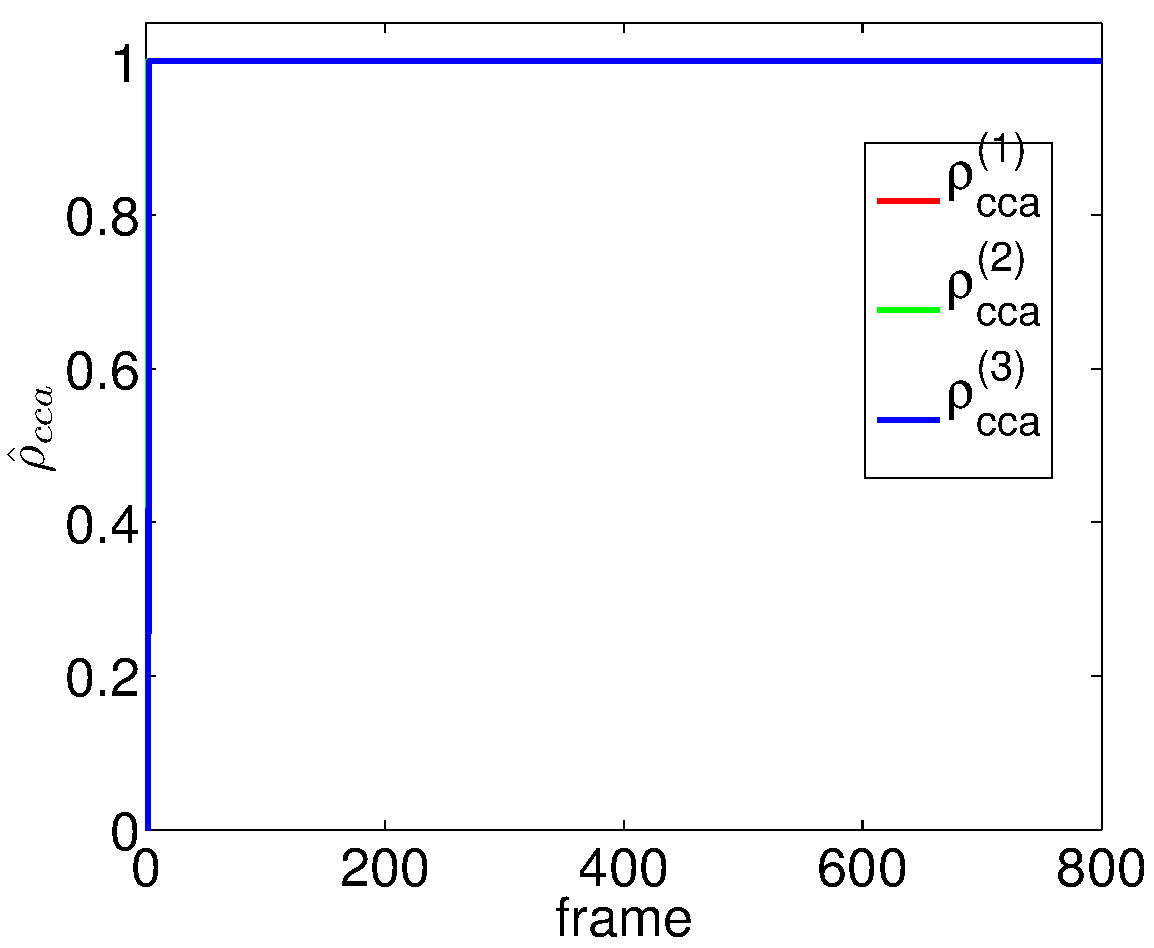
\includegraphics[width=0.47\textwidth]{chpt4_det_corr/figs/flashing_cca_corrs.pdf}
    }
    \subfigure[ICCA]{
      \label{fig:chpt4:flashing_icca_corrs}
      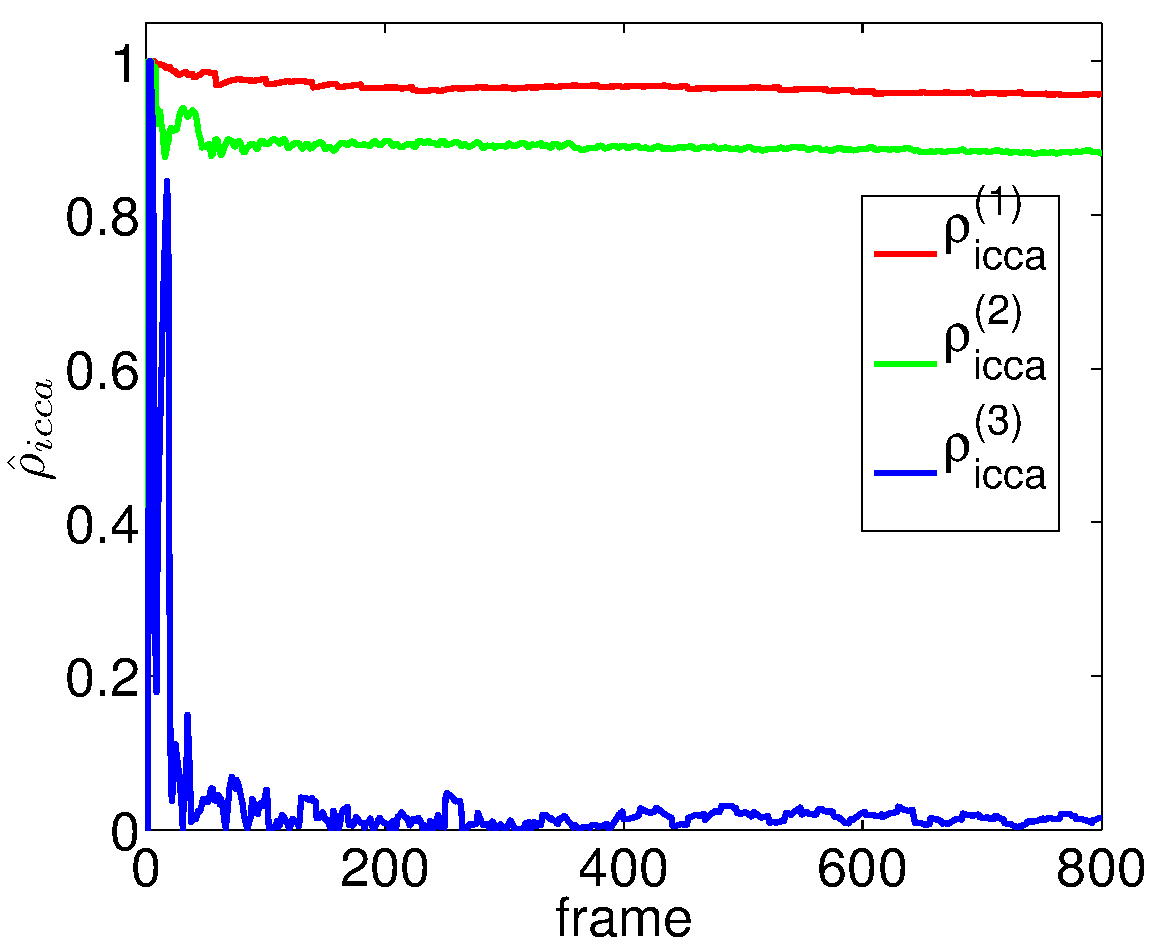
\includegraphics[width=0.47\textwidth]{chpt4_det_corr/figs/flashing_icca_corrs.pdf}
    }   
    \caption{(a) Top three singular values returned by empirical CCA as defined in
      (\ref{eq:chpt4:rhohatcca}). As we are in the sample deficient regime, these singular
      values are deterministically 1. (b) Top three singular values returned by ICCA as
      defined in (\ref{eq:chpt4:rhohaticca}). ICCA correctly identifies two sources of
      correlation.}
    \label{fig:chpt4:flashing_corrs}
  \end{center}
\end{figure}

Using these correlation coefficients, we determine which ones are significant for a
significance level of $\alpha=0.01$ using (\ref{eq:chpt4:khats}). Unsurprisingly, all
correlations returned by empirical CCA are insignificant and we do not plot the
results. However, we plot whether the ICCA correlations are significant in Figure
\ref{fig:chpt4:flashing_sigs}. After about 20 frames, ICCA identifies 2 significant
correlations. Similar to Figures \ref{fig:chpt4:ul_overlay} and
\ref{fig:chpt4:ur_overlay}, we overlay the thresholded unit-norm canonical vectors onto
the original images in Figures \ref{fig:chpt4:flashing_cca} and
\ref{fig:chpt4:flashing_icca} for empirical CCA and ICCA, respectively. The empirical CCA
canonical vectors appear to be very random and noisy. The canonical vector corresponding
to the largest ICCA correlation selects the pixels of the shared flashing camera.

\begin{figure}
  \begin{center}
    \subfigure[ICCA]{
      \label{fig:chpt4:flashing_icca_sig}
      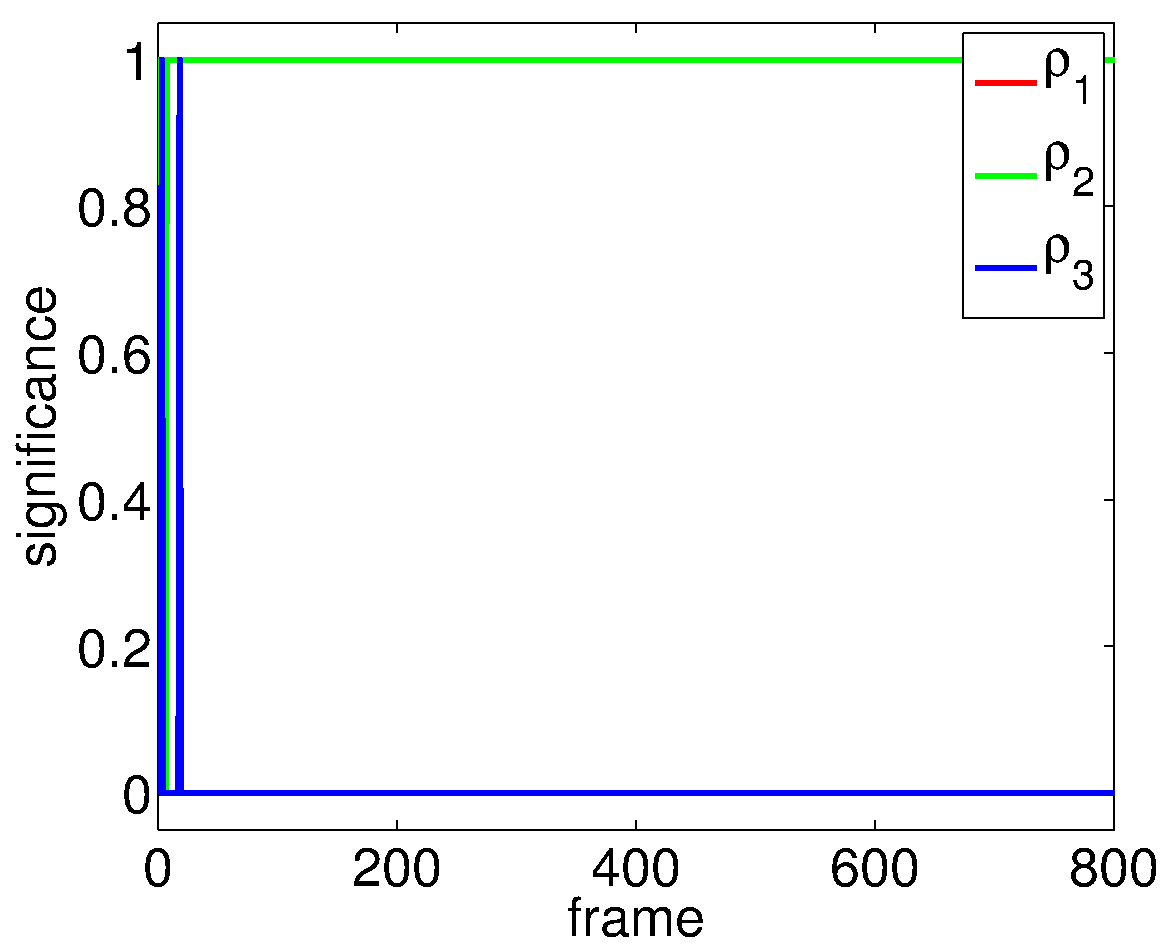
\includegraphics[width=0.47\textwidth]{chpt4_det_corr/figs/flashing_icca_sig.pdf}
    }
    \subfigure[ICCA - first 50 frames]{
      \label{fig:chpt4:flashing_cca_sig}
      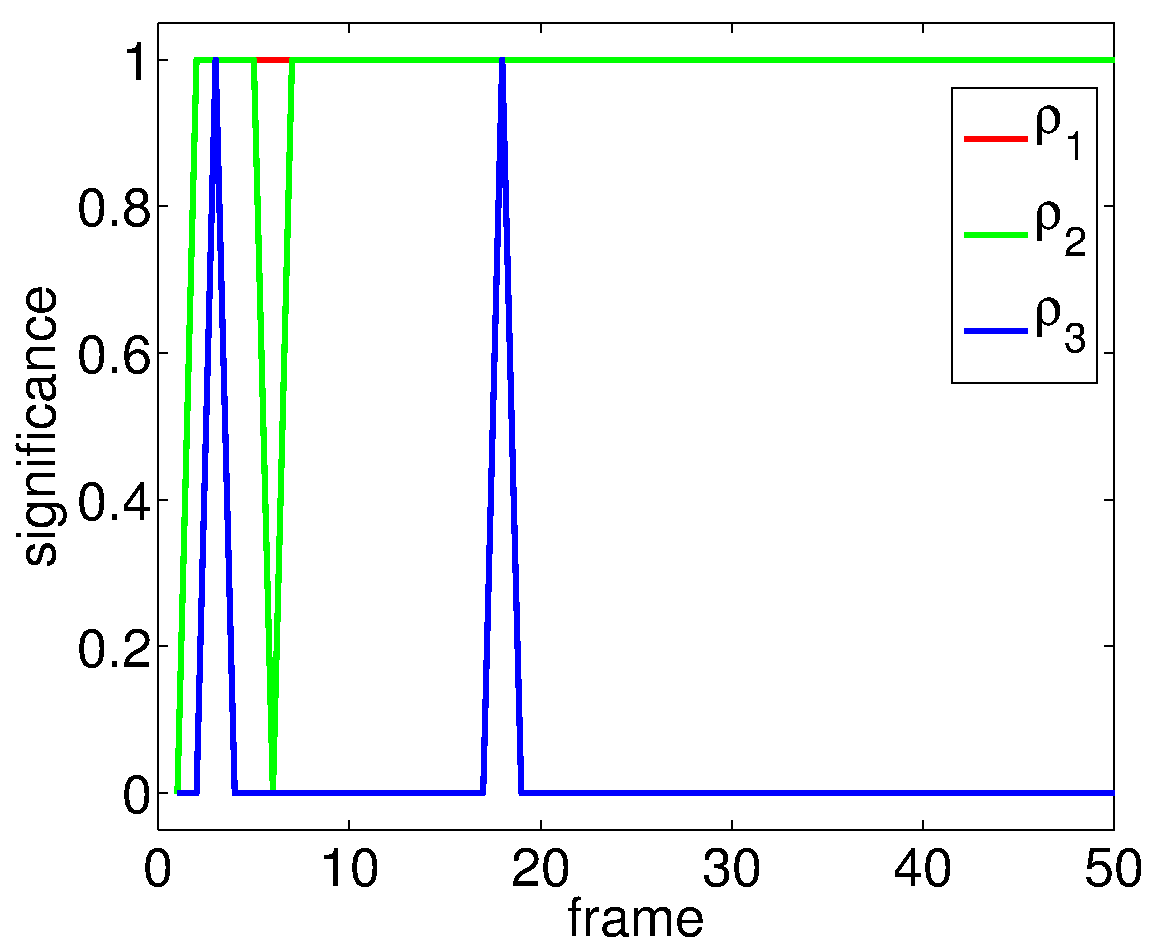
\includegraphics[width=0.47\textwidth]{chpt4_det_corr/figs/flashing_icca_sig_zoom.pdf}
    }   
    \caption{Significance of the top singular value returned by ICCA in Figure
      \ref{fig:chpt4:flashing_icca_corrs} using (\ref{eq:chpt4:khats}) with $\alpha=0.01$. A
      value of zero represents that the singular value is not significant. A value of one
      represents that the singular value is significant. (a) Significance over all 800
      frame. (b) Zoomed in to the first 50 frames in (a).}
    \label{fig:chpt4:flashing_sigs}
  \end{center}
\end{figure}

\begin{figure}
  \begin{center}
    \subfigure[Left Camera]{
      \label{fig:chpt4:flashing_left_cca}
      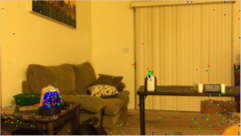
\includegraphics[width=0.47\textwidth]{chpt4_det_corr/figs/flashing_left_cca.png}
    }
    \subfigure[Right Camera]{
      \label{fig:chpt4:flashing_right_cca}
      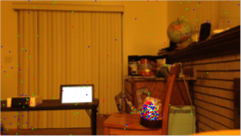
\includegraphics[width=0.47\textwidth]{chpt4_det_corr/figs/flashing_right_cca.png}
    }   
    \caption{Top 3 threholded empirical CCA canonical vectors overlayed on the original
      scene after 800 frames as computed in (\ref{eq:chpt4:cca_vects}). The red pixels
      correspond to the vector with the highest correlation, the green pixels correspond
      to the vector with the second highest correlation, and the blue pixels correspond to
      the vector with the third highest correlation. We use a threshold of
      $\log(p)/\sqrt{p}$ where $p=32400$ pixels.}
    \label{fig:chpt4:flashing_cca}
  \end{center}
\end{figure}

\begin{figure}
  \begin{center}
    \subfigure[Left Camera]{
      \label{fig:chpt4:flashing_left_icca}
      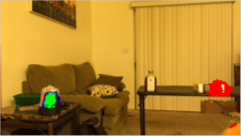
\includegraphics[width=0.47\textwidth]{chpt4_det_corr/figs/flashing_left_icca.png}
    }
    \subfigure[Right Camera]{
      \label{fig:chpt4:flashing_right_icca}
      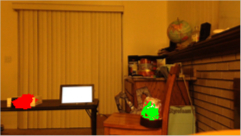
\includegraphics[width=0.47\textwidth]{chpt4_det_corr/figs/flashing_right_icca.png}
    }   
    \caption{Top 2 threholded ICCA canonical vectors overlayed on video after 800 frames
      as computed in (\ref{eq:chpt4:icca_vects}). The red pixels correspond to the vector
      with the highest correlation and the green pixels correspond to the vector with the
      second highest correlation. We use a threshold of $\log(p)/\sqrt{p}$ where $p=32400$
      pixels.}
    \label{fig:chpt4:flashing_icca}
  \end{center}
\end{figure}


Given that our experiment setup has only one shared flashing light, it is initially
surprising that ICCA returns a second significant correlation. Examining the canonical
vector overlay in Figure \ref{fig:chpt4:flashing_icca}, we observe that this correlation
corresponds to RPL and BPL. Figure \ref{fig:chpt4:flashing_v} examines the right singular
vectors returned by PCA corresponding to RPL and BPL. We observe that these light sources
have approximately the same period and even though they were started at random times, they
are in approximate antiphase, making them correlated. This is especially interesting
because neither camera can see both sources, but ICCA is still able to reveal a latent
correlation inherent in the period and phase of these lights.

\begin{figure}
  \begin{center}
      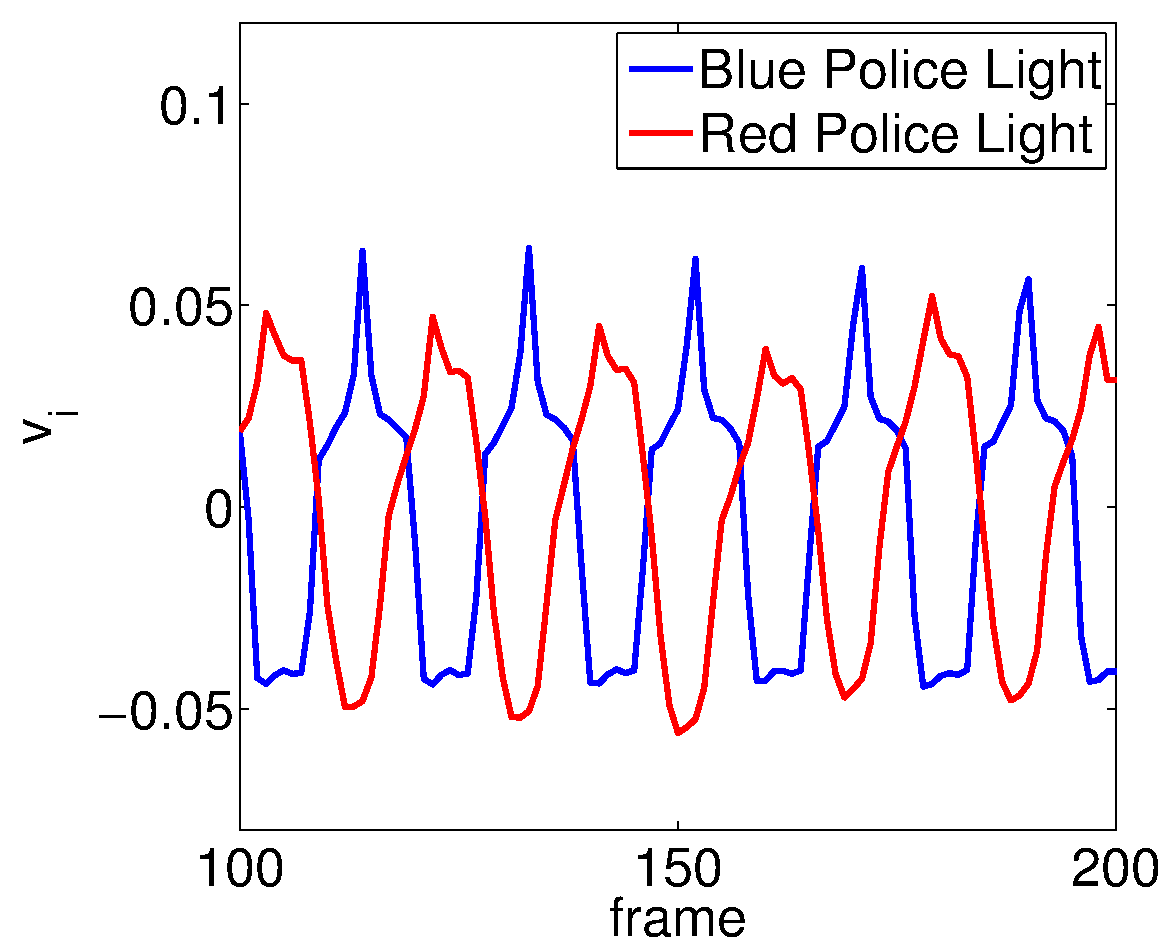
\includegraphics[width=0.47\textwidth]{chpt4_det_corr/figs/flashing_v.pdf}
    \caption{A portion of the right singular vectors of $X_{\text{left}}$ (blue) and
      $Y_{\text{right}}$ (red) corresponding the flashing police lights in each camera
      view. Both sources have very similar periods and are approximately in antiphase and
      therefore are correlated. }
    \label{fig:chpt4:flashing_v}
  \end{center}
\end{figure}

\subsection{Controlled Flashing Lights with Missing Data}

Using the same dataset in the previous section, we add missing data to each frame
independently. We set $\gamma=\gamma_x=\gamma_y=0.75$ so that about 25\% of the pixels are
set to 0. We generate the missing pixels independently for each camera and for each
frame. We then process the data exactly as above without missing data. We note that in
this setup, our light sources do not obey the low-coherence condition, but we still run
ICCA to demonstrate it's robustness. Particularly, source PH1 is very small and it's
signal is very spiked and violates the low-coherence assumption the most. It is
unsurprising that it is not detected by PCA, as we will see.

Figure \ref{fig:chpt4:flashing_miss} plots an example of a frame for each camera with
missing data. It is much more difficult to make out the scene even while retaining 75\% of
the data. Figure \ref{fig:chpt4:flashing_pca_miss} overlays the thresholded PCA vectors
onto each camera after 800 frames. For the right camera, these vectors still identify all
three visible sources. However for the left camera, we only identify BPL and PH2. This
makes sense because PH1 drastically violates the low-coherence condition. However, as this
signal is not correlated with the others, we can still attempt to use ICCA to find
correlated signals.

\begin{figure}
  \begin{center}
    \subfigure[Left Camera]{
      \label{fig:chpt4:flashing_lmiss}
      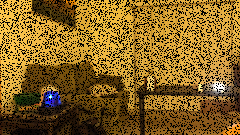
\includegraphics[width=0.47\textwidth]{chpt4_det_corr/figs/flashing_lmiss.png}
    }
    \subfigure[Right Camera]{
      \label{fig:chpt4:flashing_rmiss}
      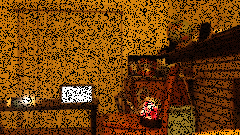
\includegraphics[width=0.47\textwidth]{chpt4_det_corr/figs/flashing_rmiss.png}
    }   
    \caption{Left and right camera views of our five sources in the presence of missing
      data.}
    \label{fig:chpt4:flashing_miss}
  \end{center}
\end{figure}

\begin{figure}
  \begin{center}
    \subfigure[Left Camera]{
      \label{fig:chpt4:flashing_left_cca}
      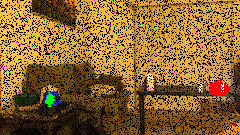
\includegraphics[width=0.47\textwidth]{chpt4_det_corr/figs/flashing_lmiss_pca.png}
    }
    \subfigure[Right Camera]{
      \label{fig:chpt4:flashing_right_cca}
      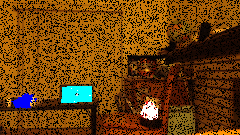
\includegraphics[width=0.47\textwidth]{chpt4_det_corr/figs/flashing_rmiss_pca.png}
    }   
    \caption{Top 3 threholded PCA vectors overlayed on each video after 800 frames. This
      is analogous to Figures \ref{fig:chpt4:flashing_UL} and \ref{fig:chpt4:flashing_UR}
      but with missing data. Again we use the threshold $\log(p)/\sqrt{p}$ for
      $p=32400$. A different color is used for the every vector. We note that the middle
      source of the left camera violates the low-coherence assumption in Assumption
      \ref{assum:chpt4:coher} and so PCA does not detect it.}
    \label{fig:chpt4:flashing_pca_miss}
  \end{center}
\end{figure}

Figure \ref{fig:chpt4:flashing_cca_miss} overlays the thresholded canonical vectors
corresponding to the top 2 empirical CCA canonical correlations onto the original scene after 800
frames. Unsurprisingly, empirical CCA is still unable to detect the two correlated signals because
in this regime the top correlations are deterministically one and the corresponding
canonical vectors are uninformative. However, ICCA is able to detect our correlated
signals even in the presence of missing data. Figure \ref{fig:chpt4:flashing_icca_miss}
overlays the thresholded canonical vectors corresponding to the top 2 ICCA canonical
correlations onto the original scene after 800 frames. The colored pixels clearly identify
our two sources of correlation. 

\begin{figure}
  \begin{center}
    \subfigure[Left Camera]{
      \label{fig:chpt4:flashing_left_cca}
      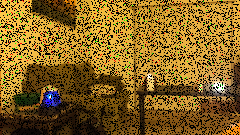
\includegraphics[width=0.47\textwidth]{chpt4_det_corr/figs/flashing_lmiss_cca.png}
    }
    \subfigure[Right Camera]{
      \label{fig:chpt4:flashing_right_cca}
      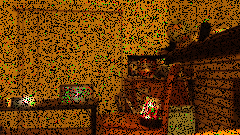
\includegraphics[width=0.47\textwidth]{chpt4_det_corr/figs/flashing_rmiss_cca.png}
    }   
    \caption{Top 2 threholded empirical CCA canonical vectors overlayed on missing data
      video as computed in (\ref{eq:chpt4:cca_vects}). Again we use the threshold
      $\log(p)/\sqrt{p}$ for $p=32400$. The red pixels correspond to the vector with the
      highest correlation and the green pixels correspond to the vector with the second
      highest correlation in Figure \ref{fig:chpt4:flashing_cca_miss_svs}.}
    \label{fig:chpt4:flashing_cca_miss}
  \end{center}
\end{figure}

\begin{figure}
  \begin{center}
    \subfigure[Left Camera]{
      \label{fig:chpt4:flashing_left_icca_miss}
      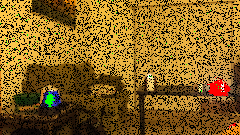
\includegraphics[width=0.47\textwidth]{chpt4_det_corr/figs/flashing_lmiss_icca.png}
    }
    \subfigure[Right Camera]{
      \label{fig:chpt4:flashing_right_icca_miss}
      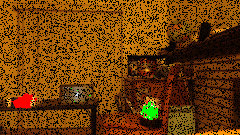
\includegraphics[width=0.47\textwidth]{chpt4_det_corr/figs/flashing_rmiss_icca.png}
    }   
    \caption{Top 2 threholded ICCA canonical vectors overlayed on missing data video as
      computed in (\ref{eq:chpt4:icca_vects}). Again we use the threshold
      $\log(p)/\sqrt{p}$ for $p=32400$. The red pixels correspond to the vector with the
      highest correlation and the green pixels correspond to the vector with the second
      highest correlation in Figure \ref{fig:chpt4:flashing_cca_miss_svs}.}
    \label{fig:chpt4:flashing_icca_miss}
  \end{center}
\end{figure}

Figure \ref{fig:chpt4:flashing_corrs_miss} plot the top 3 canonical correlations for
empirical CCA and ICCA. Unsurprisingly, the correlations reported by empirical CCA are 1
and are not significant. We plot the corresponding significance of the ICCA correlations
in Figure \ref{fig:chpt4:flashing_sigs_miss}. From these two figures, we see that ICCA is
very quickly able to determine that the shared source PH1 is correlated. At first, this is
the only significant correlation. However, after about 200 frames (about 7 seconds), the
correlation corresponding to the police lights becomes significant.

\begin{figure}
  \begin{center}
    \subfigure[CCA]{
      \label{fig:chpt4:flashing_cca_miss_svs}
      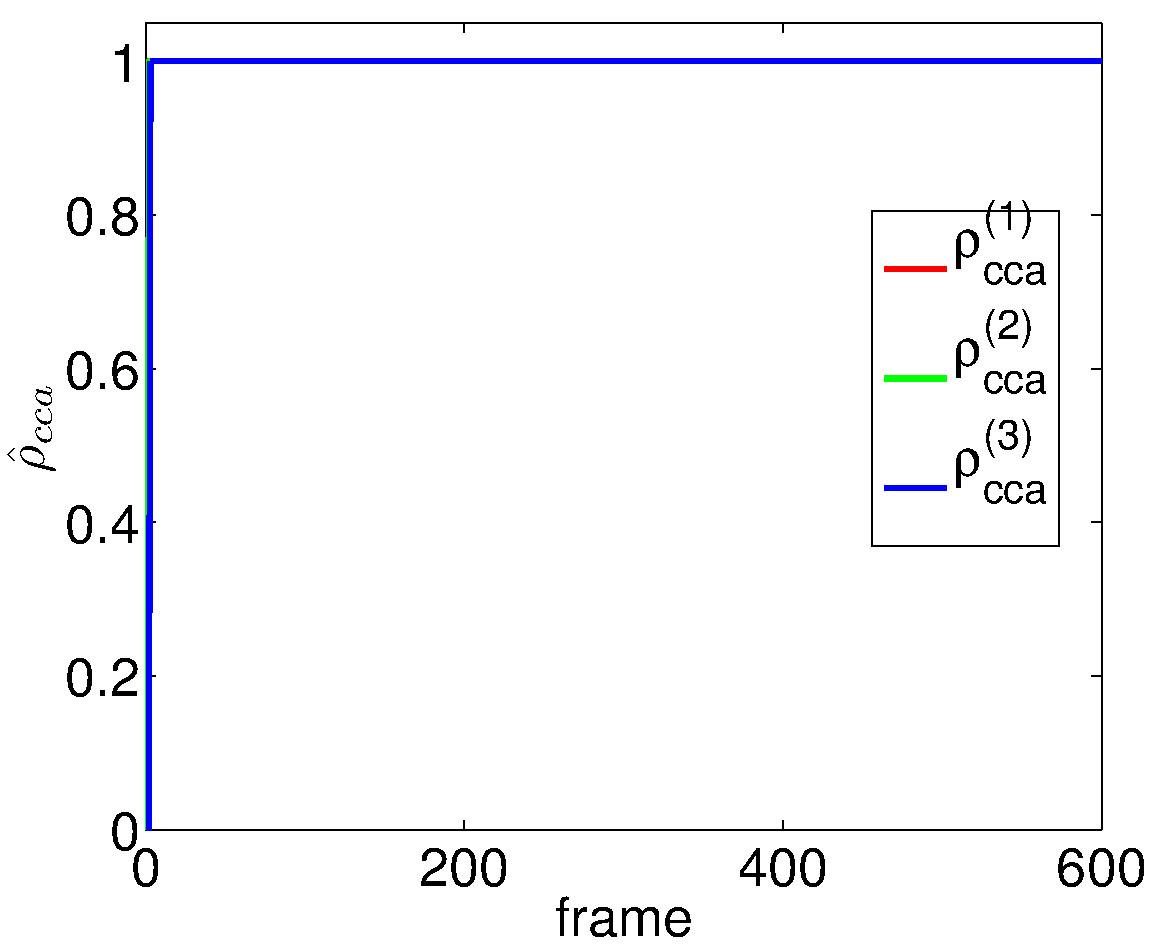
\includegraphics[width=0.47\textwidth]{chpt4_det_corr/figs/cca_corrs_miss.pdf}
    }
    \subfigure[ICCA]{
      \label{fig:chpt4:flashing_icca_miss_svs}
      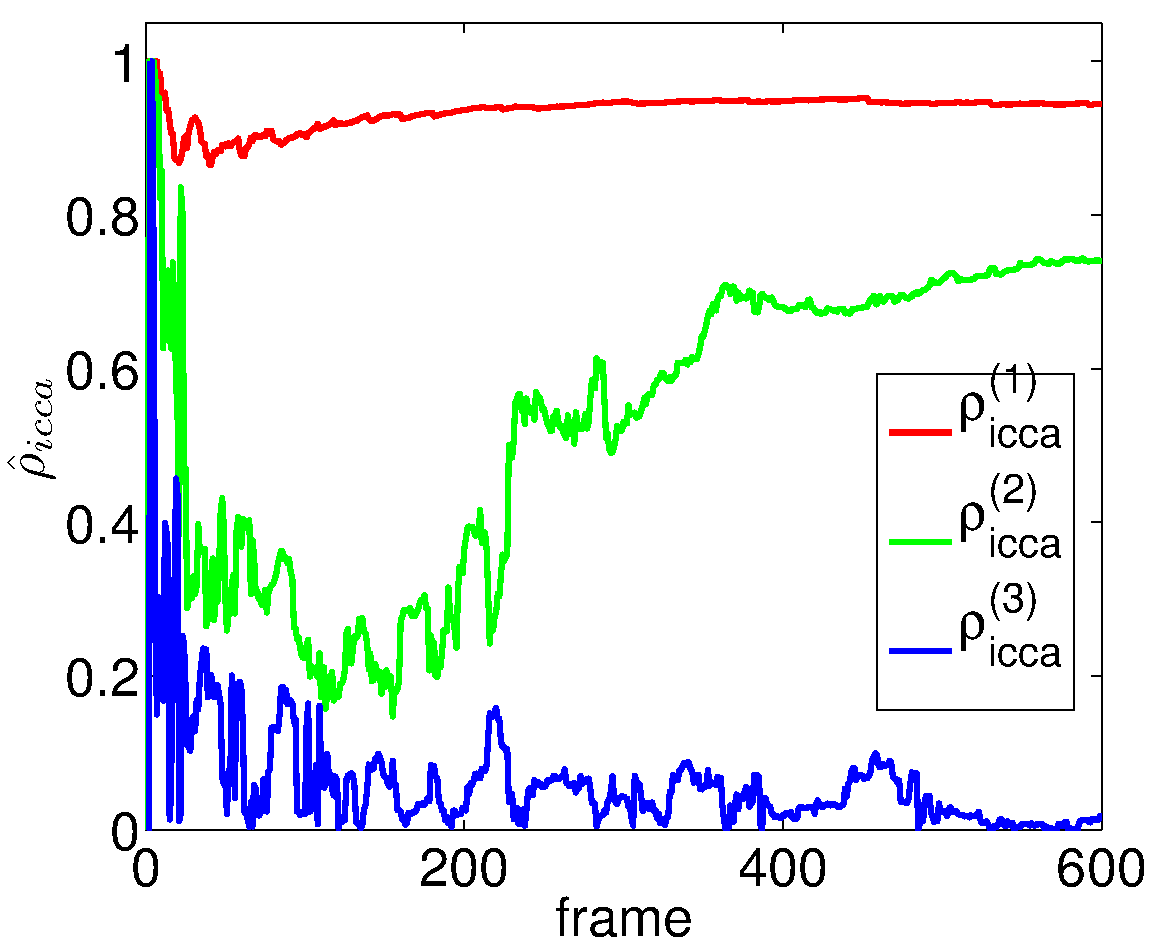
\includegraphics[width=0.47\textwidth]{chpt4_det_corr/figs/icca_corrs_miss.pdf}
    }
    \caption{(a) Top three singular values returned by empirical CCA as defined in
      (\ref{eq:chpt4:rhohatcca}). As we are in the sample deficient regime, these singular
      values are deterministically 1. (b) Top three singular values returned by ICCA as
      defined in (\ref{eq:chpt4:rhohaticca}). ICCA correctly identifies two sources of
      correlation. As our data matrices now have missing data, it takes more frames for
      ICCA to identify the two sources of correlations.}
    \label{fig:chpt4:flashing_corrs_miss}
  \end{center}
\end{figure}

\begin{figure}
  \begin{center}
    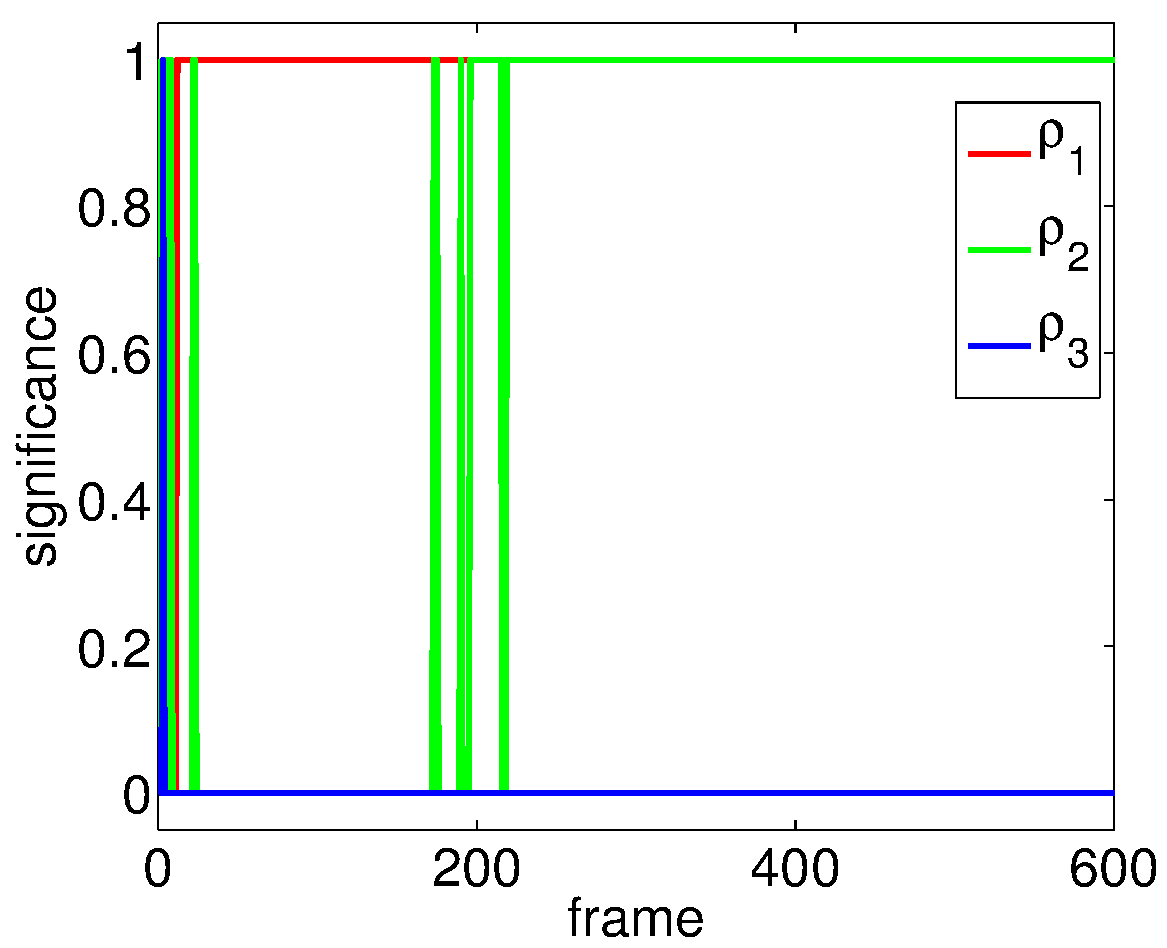
\includegraphics[width=0.47\textwidth]{chpt4_det_corr/figs/icca_sigs_miss.pdf}
    \caption{Significance of the top singular value returned by ICCA in Figure
      \ref{fig:chpt4:flashing_icca_miss_svs} using (\ref{eq:chpt4:khats}) with $\alpha=0.01$. A
      value of zero represents that the singular value is not significant. A value of one
      represents that the singular value is significant.}
    \label{fig:chpt4:flashing_sigs_miss}
  \end{center}
\end{figure}

\subsection{Controlled Audio Visual Experiment}

Similar to the flashing light experiment, we verify the effectiveness of ICCA with an
audio visual controlled experiment. In this experiment, we play an audio sequence
containing three different pure-tones, each amplitude modulated (AM) at a different
frequency. In addition, we add uncorrelated coffee shop noise
\footnote{https://www.youtube.com/watch?v=TpdFVSi7PZ8}. In the video sequence there
are two flashing block-M's, one of which is flashing at the same AM frequency as one of
the pure tone audio signals.  The audio sequence is sampled at 44.1kHz and the images are
each $553\times1000$ pixels, for a total of 20 seconds. Figure \ref{fig:chpt4:av_scene} shows
the images and identifies the two  sources. Figure \ref{fig:chpt4:av_spectrograms} plots the
full spectrogram of our audio signal and zooms in on a smaller portion of the spectrum to
see the three AM signals, which are described in Table \ref{tab:av_descrp}. Our audio
waveform is

\beq\label{eq:chpt4_av_total}
a(t) = \frac{1}{4}s_1(t) + \frac{1}{4}s_2(t) + \frac{1}{4}s_3(t) + \frac{1}{4}n(t)
\eeq
where 
\beq\label{eq:chpt4:av_signals}\ba
& s_1(t) = |\sin(2\pi t/2)|\sin\left(2\pi\left(250t\right)\right)\\
& s_2(t) = |\cos(2\pi (3/2t))|\sin\left(2\pi\left(400t\right)\right)\\
& s_3(t) = |\cos(2\pi (5/2 t))|\sin\left(2\pi\left(550t\right)\right)\\
& n(t) = \text{coffee shop noise}. \\
\ea\eeq

\begin{figure}
  \centering
  
\includegraphics[width=0.47\textwidth]{chpt4_det_corr/figs/av_video.png}
  \caption{Still shot of the video. The block M on the left is amplitude modulated at 1
    Hz, the same rate as $s_1(t)$ in (\ref{eq:chpt4:av_signals}), while the block M on the
    right is amplitude modulate at 2.15 Hz, which is different than all other audio and
    visual sources.}
  \label{fig:chpt4:av_scene}
\end{figure}

\begin{figure}
  \begin{center}
    \subfigure[Full Spectrogram]{
      \label{fig:chpt4:av_raw}
      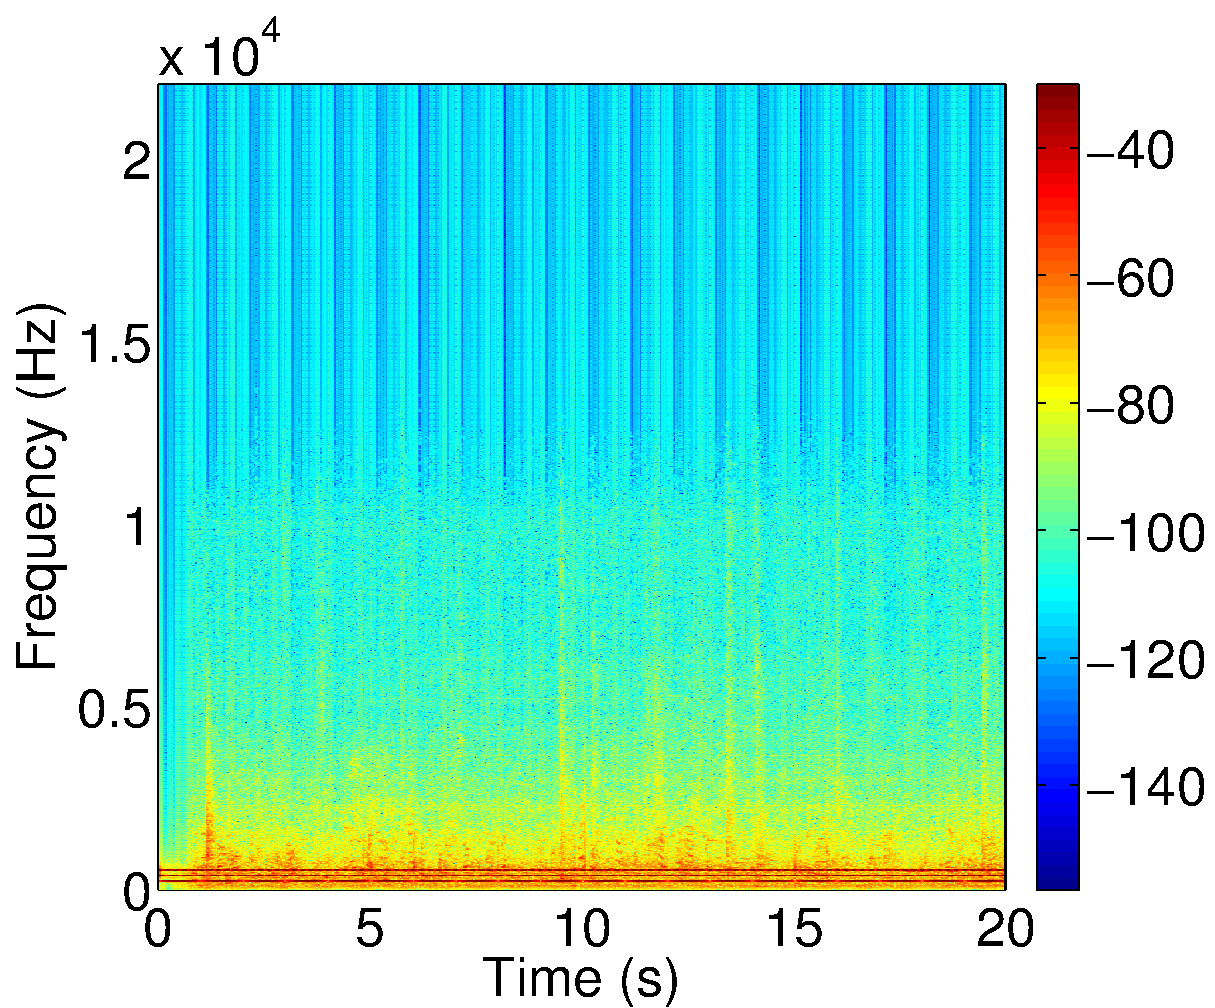
\includegraphics[width=0.47\textwidth]{chpt4_det_corr/figs/av_full_spect.pdf}
    }
    \subfigure[Zoomed Spectrogram]{
      \label{fig:chpt4:av_man}
      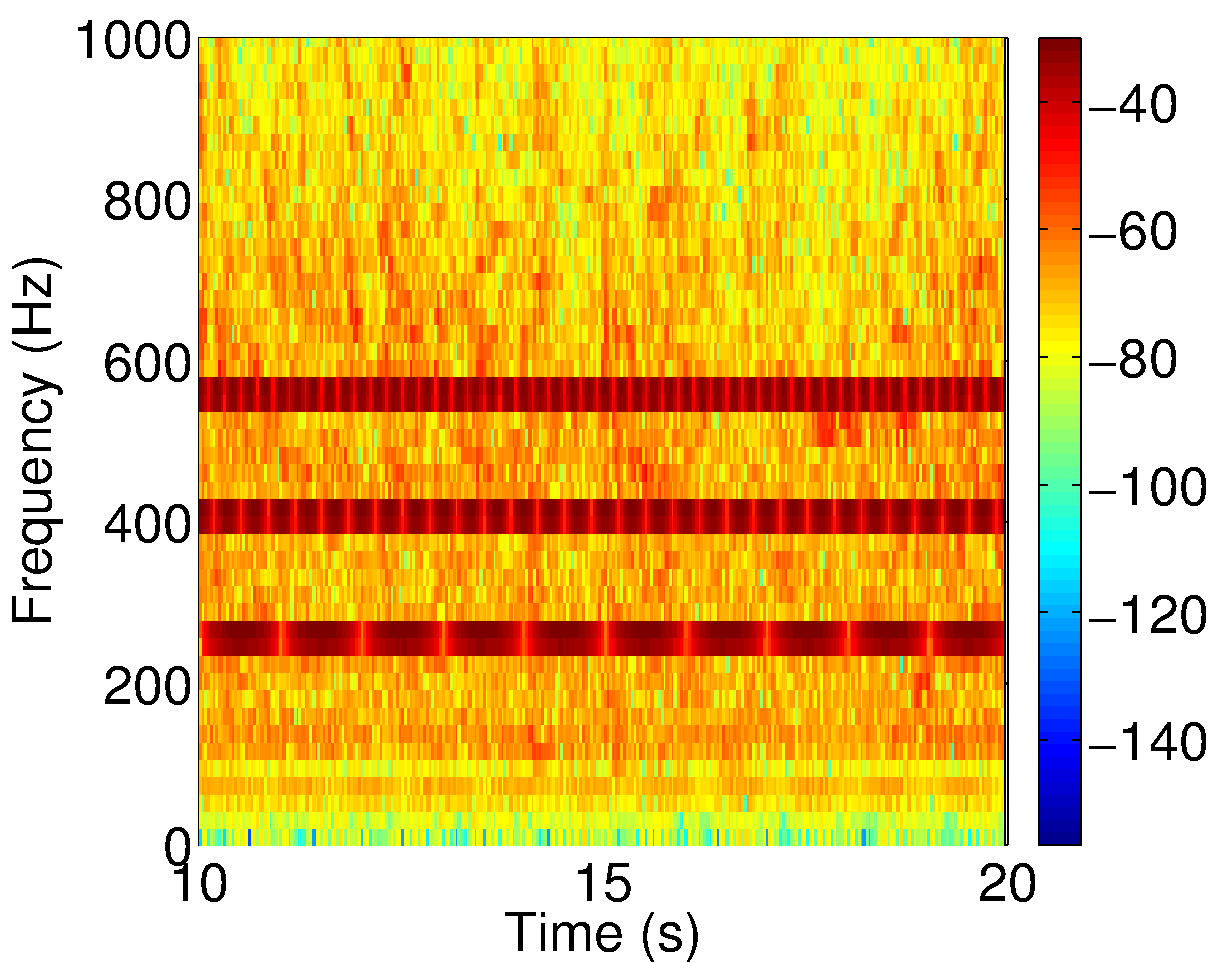
\includegraphics[width=0.47\textwidth]{chpt4_det_corr/figs/av_zoom_spect.pdf}
    }   
    \caption{(a) Full spectrogram of the audio signal in (\ref{eq:chpt4_av_total}). (b)
      Zoomed in spectrogram of (a) to see the 3 audio sources at 250 Hz, 400 Hz, and 550
      Hz. Each sources is also amplitude modulated at a different frequency as described
      in (\ref{eq:chpt4:av_signals}).}
    \label{fig:chpt4:av_spectrograms}
  \end{center}
\end{figure}


\begin{table*}[ht!]
\centering
\begin{tabular}{c|c|c}\toprule
Type & Source & AM Frequency\\
\midrule
Visual & Left Block M & 1 Hz\\
& Right Block M & 2.15 Hz\\
\midrule
Audio & 250 Hz pure tone & 1 Hz\\
& 400 Hz pure tone & 3 Hz\\
& 550 Hz pure tone & 7 Hz\\
& coffee shop noise &\\
\bottomrule
\end{tabular}
\caption{Summary of the audio and visual sources and their amplitude modulated
  signals. The audio sources are described in (\ref{eq:chpt4:av_signals}) and the video
  sources are shown in Figure \ref{fig:chpt4:av_scene}. The 250 Hz pure tone is amplitude
  modulated at the same frequency as the left block M and is thus correlated with it.}
\label{tab:av_descrp}
\end{table*}


To post-process the video data, we first converted the video streams to grayscale and then
downsampled each spatial dimension by a factor of 4, resulting in a resolution of
$133\times 250$. We then ignore the first and last second of data and vectorized the image
and stacked the resulting 540 frames into a data matrix of dimension $33250 \times
540$. Finally, we subtract the mean from the video dataset so that we may run PCA, empirical CCA,
and ICCA on the zero-mean dataset, $X_{\text{video}}$.

To post-process the audio data, we separate the audio stream into equal window sizes of
1470 time points centered on every 1/30 second of data. On each 1470 time point segment,
we run a 2048 point FFT and take the magnitude of the first 1025 points as a feature
vector. We process the 18 seconds of data, stack the feature vectors into a matrix, and
then subtract the mean, resulting in a $1025 \times 540$ matrix $Y_{\text{audio}}$.

First, we run PCA on $X_{\text{video}}$ and $Y_{\text{audio}}$. Figure \ref{fig:chpt4:av_sv}
plots the singular value of each dataset. From our setup, we know that the video dataset
has 2 signals and the audio dataset has 3 sources. Figure \ref{fig:chpt4:av_vu} plots
the singular vector heatmaps corresponding to the top 2 singular values of
$X_{\text{video}}$. These heatmaps clearly identify the two block M's. We then
threshold the absolute value of the singular vectors with the threshold $1/\sqrt{p}$
and overlay it on top of the original scene. Similarly, Figure \ref{fig:chpt4:av_audio_pca}
plots the singular vectors of $Y_{\text{audio}}$ corresponding to the top 3 singular
values. By thresholding these singular vectors, we create audio filters, as Figure
\ref{fig:chpt4:av_audio_pca_mask} shows. 

\begin{figure}
  \begin{center}
    \subfigure[Video]{
      \label{fig:chpt4:ul1}
      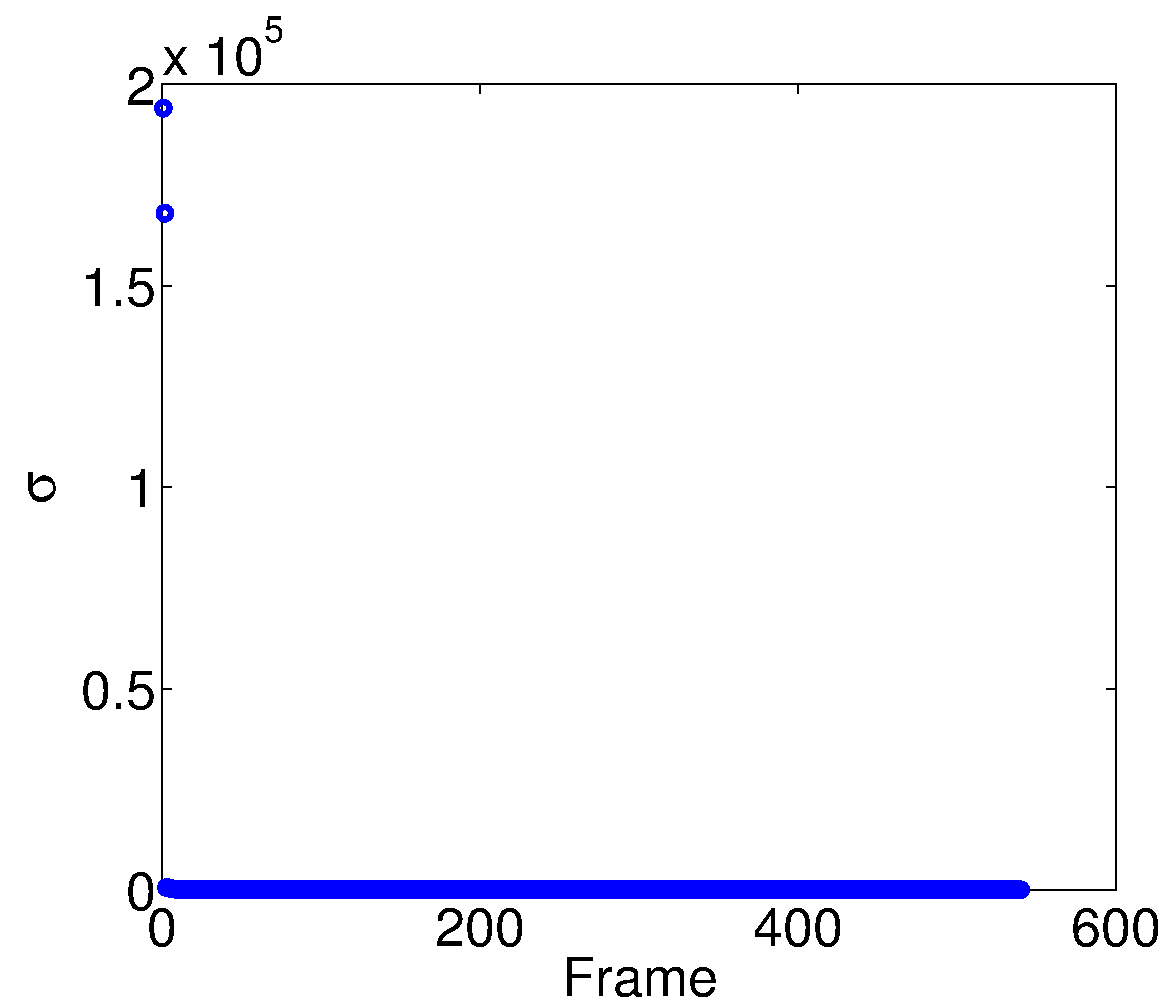
\includegraphics[width=0.47\textwidth]{chpt4_det_corr/figs/av_vsv.pdf}
    }
    \subfigure[Audio]{
      \label{fig:chpt4:ul2}
      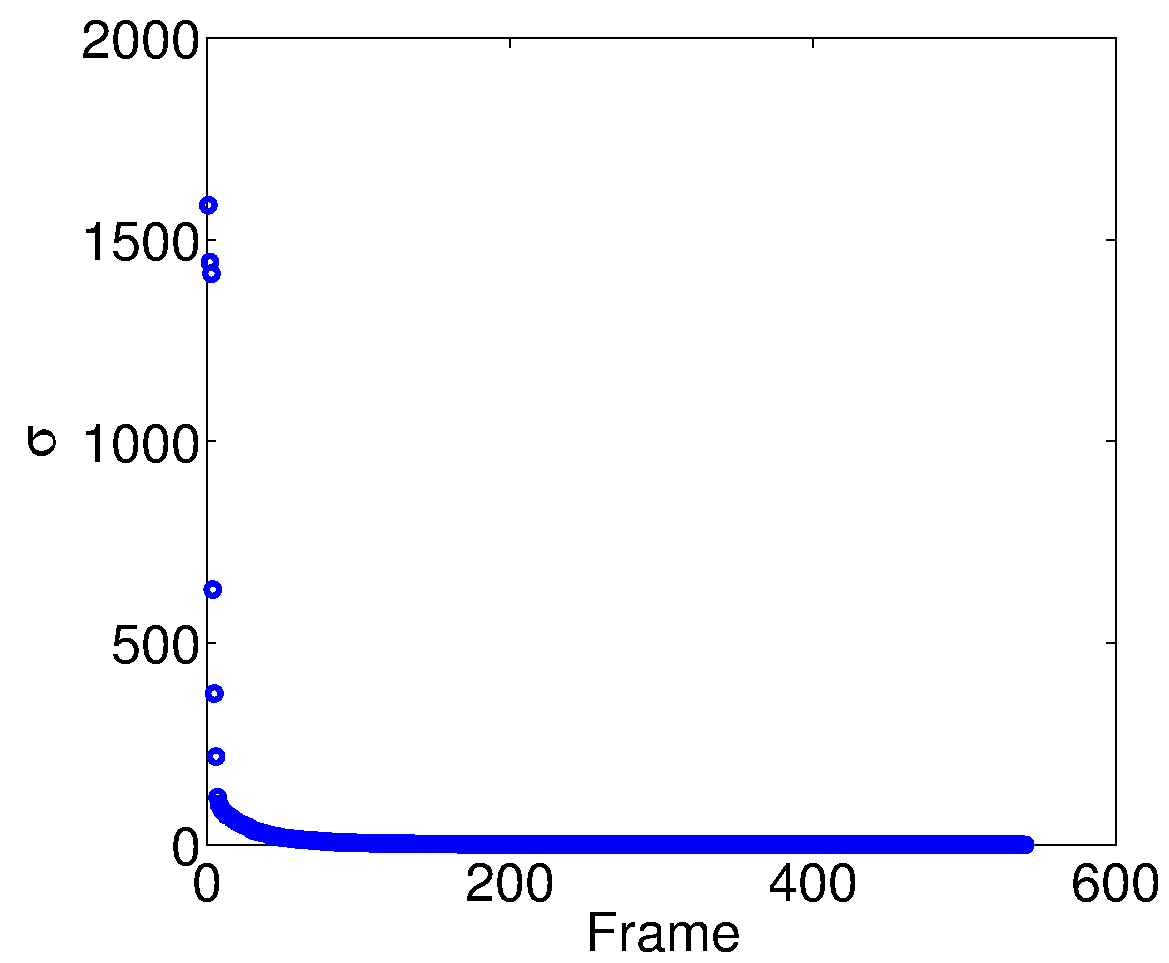
\includegraphics[width=0.47\textwidth]{chpt4_det_corr/figs/av_asv.pdf}
    }   
    \caption{Singular value spectra of $X_{\text{video}}$ and $Y_{\text{audio}}$.}
    \label{fig:chpt4:av_sv}
  \end{center}
\end{figure}

\begin{figure}
  \begin{center}
    \subfigure[$u_1$]{
      \label{fig:chpt4:av_vu1}
      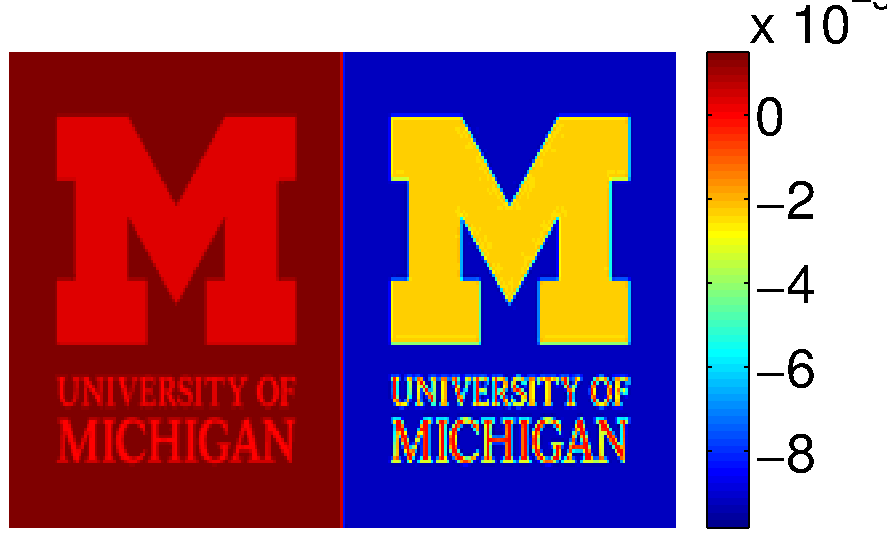
\includegraphics[width=0.47\textwidth]{chpt4_det_corr/figs/av_vu1.pdf}
    }
    \subfigure[$u_2$]{
      \label{fig:chpt4:av_vu2}
      \includegraphics[width=0.47\textwidth]{chpt4_det_corr/figs/av_vu2.pdf}
    }   
    \subfigure[$u_3$]{
      \label{fig:chpt4:av_vu_overlay}
      \includegraphics[width=0.47\textwidth]{chpt4_det_corr/figs/av_vu_overlay.png}
    }
    \caption{(a)-(b)) Left singular vectors of $X_{\text{video}}$ corresponding to the top
      2 singular values. (c) Thresholded singular vectors from (a)-(b) overlayed onto
      original scene with pixels from (a) in red and pixels from (b) in green. We use the
      threshold $\log(p)/\sqrt{p}$ for $p=33250$. These vectors correspond to the 2 block M's.}
    \label{fig:chpt4:av_vu}
  \end{center}
\end{figure}

\begin{figure}
  \begin{center}
    \subfigure[Audio principle components]{
      \label{fig:chpt4:av_audio_pca_full}
      \includegraphics[width=0.47\textwidth]{chpt4_det_corr/figs/av_pca_audio.pdf}
    }
    \subfigure[Zoomed-in of (a)]{
      \label{fig:chpt4:av_audio_pca_zoom}
      \includegraphics[width=0.47\textwidth]{chpt4_det_corr/figs/av_pca_zoom_audio.pdf}
    }   
    \subfigure[Example Filter]{
      \label{fig:chpt4:av_audio_pca_mask}
      \includegraphics[width=0.47\textwidth]{chpt4_det_corr/figs/av_pca_mask_audio.pdf}
    }   
    \caption{(a) Left singular vectors of $Y_{\text{audio}}$ corresponding to the top 3
      singular values. (b) Zoomed in version of (a) to see the three audio sources. (c)
      Masked principle component formed by thresholding the singular vectors with
      $\sqrt{\log(q)/q}$ for $q=1025$.}
    \label{fig:chpt4:av_audio_pca}
  \end{center}
\end{figure}


However, PCA does not provide any information about whether the identified audio visual
signals are correlated. To identify such correlations, we run empirical CCA and ICCA after each new
video frame. For frame $\ell$, we construct the $33250\times\ell$ submatrix
$X_{\text{video}}^\ell$ and $1025\times\ell$ submatrix $Y_{\text{audio}}^\ell$ by taking
the matrix of the first $\ell$ original vectorized frames and zero meaning it. We then use
these matrices as the input to empirical CCA and ICCA. Using knowledge of our experimental
setup, we set $\kxhat=2$ and $\kyhat=3$. Figure \ref{fig:chpt4:av_corrs} plots the top 2
correlation coefficients returned by empirical CCA and ICCA over the first 540
frames. Intuitively, empirical CCA returns perfect correlation as we have only a few
frames but a large dimension (pixels).



\begin{figure}
  \begin{center}
    \subfigure[Empirical CCA]{
      \label{fig:chpt4:av_cca_corrs}
      \includegraphics[width=0.47\textwidth]{chpt4_det_corr/figs/av_cca_corrs.pdf}
    }
    \subfigure[ICCA]{
      \label{fig:chpt4:av_icca_corrs}
      \includegraphics[width=0.47\textwidth]{chpt4_det_corr/figs/av_icca_corrs.pdf}
    }   
    \caption{(a) Top two singular values returned by empirical CCA as defined in
      (\ref{eq:chpt4:rhohatcca}). As we are in the sample deficient regime, these singular
      values are deterministically 1. (b) Top two singular values returned by ICCA as
      defined in (\ref{eq:chpt4:rhohaticca}). ICCA correctly identifies the one source of
      correlation present in the audio-video dataset.}
    \label{fig:chpt4:av_corrs}
  \end{center}
\end{figure}

While the canonical correlation coefficients returned by CCA are insignificant because we
operate in the sample deficient regime, we may use (\ref{eq:chpt4:khats}) to determine whether
the canonical correlation coefficients returned by ICCA are significant. Using a
significance level of $\alpha=0.01$, Figure \ref{fig:chpt4:av_sigs} plots whether the ICCA
canonical correlations are significant. Unsurprisingly, after 20 frames (2/3 seconds) we
identify the only correlated source and show that the second correlation is
insignificant. The only significant correlation corresponds to the one correlated
audio-visual signal.

\begin{figure}
  \begin{center}
    \subfigure[ICCA]{
      \label{fig:chpt4:av_icca_sig}
      \includegraphics[width=0.47\textwidth]{chpt4_det_corr/figs/av_icca_sig.pdf}
    }
    \subfigure[ICCA - first 75 frames]{
      \label{fig:chpt4:av_cca_sig}
      \includegraphics[width=0.47\textwidth]{chpt4_det_corr/figs/av_icca_sig_zoom.pdf}
    }   
    \caption{Significance of the top singular value returned by ICCA in Figure
      \ref{fig:chpt4:av_corrs} using (\ref{eq:chpt4:khats}) with $\alpha=0.01$. A
      value of zero represents that the singular value is not significant. A value of one
      represents that the singular value is significant. (a) Significance for all 540
      frames. (b) Zoomed in of (a) to examine the first 75 frames.}
    \label{fig:chpt4:av_sigs}
  \end{center}
\end{figure}

Figure \ref{fig:chpt4:av_cca} uses the first empirical CCA canonical vectors to filter
both the audio and video stream to highlight the correlated component. Using the
thresholded first audio canonical vector as a bandpass filter, we filter the original
audio stream using the overlap-save method and plot the resulting spectrogram in Figures
\ref{fig:chpt4:av_audio_cca} and \ref{fig:chpt4:av_audio_cca_zoom}. From the spectrogram,
we see that the canonical vectors filters random frequencies and as time goes on, filter
almost everything. Similarly, we threshold the video canonical vector and plot the pixels
that are above the threshold in Figure \ref{fig:chpt4:av_video_cca}. The pixels congregate
around the text in both block M's, which is not correlated. These figures demonstrate that
empirical CCA fails to identify the pixels that are correlated to any audio source and
instead returns random filters for both the audio and video sources.

\begin{figure}
  \begin{center}
    \subfigure[Audio]{
      \label{fig:chpt4:av_audio_cca}
      \includegraphics[width=0.47\textwidth]{chpt4_det_corr/figs/av_cca_spect.pdf}
    }   
    \subfigure[Audio - zoomed]{
      \label{fig:chpt4:av_audio_cca_zoom}
      \includegraphics[width=0.47\textwidth]{chpt4_det_corr/figs/av_cca_zoom_spect.pdf}
    }   
    \subfigure[Video]{
      \label{fig:chpt4:av_video_cca}
      \includegraphics[width=0.47\textwidth]{chpt4_det_corr/figs/av_cca_overlay.png}
    }
    \caption{Thresholded canonical vectors (as computed in (\ref{eq:chpt4:cca_vects}))
      corresponding to the top singular value returned by empirical CCA in Figure
      \ref{fig:chpt4:av_cca_corrs}. We use a threshold of $\log(p)/\sqrt{p}$ for $p=33250$
      and $p=1025$ for video and audio vectors, respectively. (a) Spectrogram of the
      original audio stream filtered using the thresholded empirical CCA top canonical
      vector and the overlap-save filter method. (b) Zoomed in spectrogram of (a). (c) Red
      colored pixels represent the pixels that empirical CCA marks as correlated to the
      audio stream in (a).}
    \label{fig:chpt4:av_cca}
  \end{center}
\end{figure}

However, ICCA is able to find the underlying correlated audio-video source, as shown in
Figure \ref{fig:chpt4:av_icca}.  Just as in the empirical CCA analysis, we use the
thresholded first ICCA audio canonical vector to bandpass filter the original audio stream
using the overlap-save method and plot the resulting spectrogram in Figures
\ref{fig:chpt4:av_audio_icca} and \ref{fig:chpt4:av_audio_icca_zoom}. Unlike empirical
CCA, the ICCA audio filter correctly filters the audio to contain the correlated 250 Hz
audio tone. Figure \ref{fig:chpt4:av_video_icca} plots the pixels in our scene that are
correlated with the audio source and ICCA is able to correctly identify the left block M.

\begin{figure}
  \begin{center}
    \subfigure[Audio]{
      \label{fig:chpt4:av_audio_icca}
      \includegraphics[width=0.47\textwidth]{chpt4_det_corr/figs/av_icca_spect.pdf}
    }   
    \subfigure[Audio - zoomed]{
      \label{fig:chpt4:av_audio_icca_zoom}
      \includegraphics[width=0.47\textwidth]{chpt4_det_corr/figs/av_icca_zoom_spect.pdf}
    }   
    \subfigure[Video]{
      \label{fig:chpt4:av_video_icca}
      \includegraphics[width=0.47\textwidth]{chpt4_det_corr/figs/av_icca_overlay.png}
    }
    \caption{Thresholded canonical vectors (as computed in (\ref{eq:chpt4:icca_vects}))
      corresponding to the top singular value returned by ICCA in Figure
      \ref{fig:chpt4:av_icca_corrs}. We use a threshold of $\log(p)/\sqrt{p}$ for
      $p=33250$ and $p=1025$ for video and audio vectors, respectively. (a) Spectrogram of
      the original audio stream filtered using the thresholded ICCA top canonical vector
      and the overlap-save filter method. (b) Zoomed in spectrogram of (a). (c) Red
      colored pixels represent the pixels that ICCA marks as correlated to the audio
      stream in (a).}
    \label{fig:chpt4:av_icca}
  \end{center}
\end{figure}


\subsection{Controlled Audio Audio Experiment}

Our final experiment explores the inherent correlation between two audio streams. In this
experiment, we generate two 30 second audio sequences. Each sequence contains two
pure-tones, which are amplitude modulated (AM) at different frequencies. In addition we
add uncorrelated coffee shop noise, which is independent between each audio sequence. One
pure-tone in each sequence is AM at a shared rate, inducing correlation between the audio
sequences. The remaining pure-tones are AM at different rates, making them independent of
the shared AM tones. Our waveforms are 
\beq\label{eq:chpt4:aa_sources}\ba
&a_1(t) = \frac{1}{3}s_1(t) + \frac{1}{3}s_2(t) + \frac{1}{3}n_1(t)\\
&a_2(t) = \frac{1}{3}s_3(t) + \frac{1}{3}s_4(t) + \frac{1}{3}n_2(t)
\ea\eeq
where 
\beq\label{eq:chpt4:aa_signals}\ba
& s_1(t) = \frac{(1+\sin(2\pi t))}{2}\sin\left(2\pi\left(250t\right)\right)\\
& s_2(t) = \frac{(1+\cos(2\pi (3t))}{2}\sin\left(2\pi\left(400t\right)\right)\\
& s_3(t) = \frac{(1+\sin(2\pi t))}{2}\sin\left(2\pi\left(300t\right)\right)\\
& s_4(t) = \frac{(1+\cos(2\pi (5t))}{2}\sin\left(2\pi\left(550t\right)\right)\\
& n_1(t) = \text{independent coffee shop noise}\\
& n_2(t) = \text{independent coffee shop noise}. \\
\ea\eeq
All time sequences are generated with a sample rate of 44.1 kHz. Figure
\ref{tab:aa_descrp} plots the spectrogram of each sequence and zooms in on a smaller
portion of the spectrum to see the AM sequences. Table \ref{fig:chpt4:aa_spectrograms}
summarizes each of our signals in each audio sequences.
\begin{table*}[ht!]
\centering
\begin{tabular}{c|c|c}\toprule
View & Source & AM Frequency\\
\midrule
$a_1(t)$ & 250 Hz pure tone & 1 Hz\\
& 400 Hz pure tone & 3 Hz\\
& coffee shop noise 1&\\
\midrule
$a_2(t)$ & 300 Hz pure tone & 1 Hz\\
& 550 Hz pure tone & 5 Hz\\
& coffee shop noise 2&\\
\bottomrule
\end{tabular}
\caption{Summary of the audio sources in (\ref{eq:chpt4:aa_sources}) and their components
  in (\ref{eq:chpt4:aa_signals}). The 250 Hz pure tone in $a_1(t)$ is amplitude
  modulated at the same frequency as the 300 Hz pure tone in $a_2(t)$ and is thus
  correlated with it.}
\label{tab:aa_descrp}
\end{table*}

\begin{figure}
  \begin{center}
    \subfigure[Full Spectrogram of $a_1(t)$]{
      \label{fig:chpt4:aa1_full_spec}
      \includegraphics[width=0.47\textwidth]{chpt4_det_corr/figs/aa1_full_spect.pdf}
    }
    \subfigure[Zoomed Spectrogram of $a_1(t)$]{
      \label{fig:chpt4:aa1_spec_zoom}
      \includegraphics[width=0.47\textwidth]{chpt4_det_corr/figs/aa1_zoom_spect.pdf}
    }   
    \subfigure[Full Spectrogram of $a_2(t)$]{
      \label{fig:chpt4:aa2_full_spec}
      \includegraphics[width=0.47\textwidth]{chpt4_det_corr/figs/aa2_full_spect.pdf}
    }
    \subfigure[Zoomed Spectrogram of $a_2(t)$]{
      \label{fig:chpt4:aa2_spec_zoom}
      \includegraphics[width=0.47\textwidth]{chpt4_det_corr/figs/aa2_zoom_spect.pdf}
    }   
    \caption{(a) Full spectrogram of $a_1(t)$ defined in (\ref{eq:chpt4:aa_sources}). (b)
      Zoomed in spectrogram of $a_1(t)$ to see the 2 sources at 250 Hz and 400 Hz. (c)
      Full spectrogram of $a_2(t)$ defined in (\ref{eq:chpt4:aa_sources}) (d) Zoomed in
      spectrogram of $a_2(t)$ to see the 2 sources at 300 Hz and 550 Hz. The 250 Hz signal
      in $a_1(t)$ is amplitude modulated at the same frequency as the 300 Hz signal in
      $a_2(t)$.}
    \label{fig:chpt4:aa_spectrograms}
  \end{center}
\end{figure}

To post-process the data, we separate the audio streams into equal window sizes of 2940
time points, corresponding to a time interval of 1/15 second. On each window, we run a
4096 point FFT and take the magnitude of the first 2049 points as a feature vector. We
then stack the feature vectors for all windows into a matrix and subtract the mean,
resulting in $2049 \times 450$ matrices $X_{a_1}$ and $Y_{a_2}$.

First, we run PCA on $X_{a_1}$ and $Y_{a_2}$. Figure \ref{fig:chpt4:aa_sv} plots the singular
values of each dataset. From our setup, we know that each audio sequence has 2 pure-tone
signals plus coffee shop noise. Figure \ref{fig:chpt4:aa_pca} plots the corresponding singular
vectors for the top 2 singular vectors of each audio dataset.

\begin{figure}
  \begin{center}
    \subfigure[Video]{
      \label{fig:chpt4:aa_sv1}
      \includegraphics[width=0.47\textwidth]{chpt4_det_corr/figs/aa_sv1.pdf}
    }
    \subfigure[Audio]{
      \label{fig:chpt4:aa_sv2}
      \includegraphics[width=0.47\textwidth]{chpt4_det_corr/figs/aa_sv2.pdf}
    }   
    \caption{Singular value spectra of $X_{a_1}$ and $Y_{a_2}$.}
    \label{fig:chpt4:aa_sv}
  \end{center}
\end{figure}

\begin{figure}
  \begin{center}
    \subfigure[$X_{a_1}$ principle components]{
      \label{fig:chpt4:aa_pca1}
      \includegraphics[width=0.47\textwidth]{chpt4_det_corr/figs/aa_pca1.pdf}
    }
    \subfigure[$X_{a_1}$ zoomed-in principle components]{
      \label{fig:chpt4:aa_pca1_zoom}
      \includegraphics[width=0.47\textwidth]{chpt4_det_corr/figs/aa_pca1_zoom.pdf}
    }   
    \subfigure[$Y_{a_2}$ principle components]{
      \label{fig:chpt4:aa_pca2}
      \includegraphics[width=0.47\textwidth]{chpt4_det_corr/figs/aa_pca2.pdf}
    }
    \subfigure[$Y_{a_2}$ zoomed-in principle components]{
      \label{fig:chpt4:aa_pca2_zoom}
      \includegraphics[width=0.47\textwidth]{chpt4_det_corr/figs/aa_pca2_zoom.pdf}
    }   
    \caption{(a) Left singular vectors of $X_{a_1}$ corresponding to the top 2 singular
      values in Figure \ref{fig:chpt4:aa_sv1}. (b) Zoomed in version of (a). (c) Left
      singular vectors of $Y_{a_2}$ corresponding to the top 2 singular values in Figure
      \ref{fig:chpt4:aa_sv2}. (d) Zoomed in version of (c).}
    \label{fig:chpt4:aa_pca}
  \end{center}
\end{figure}


While the PCA vectors in Figure \ref{fig:chpt4:aa_pca} can identify sources within a
dataset, by themselves, they do not provide any information about whether the sources are
correlated between datasets. To identify such correlations, we run empirical CCA and ICCA
after each 
new video frame. For frame $\ell$, we construct the $2049\times\ell$ submatrix
$X_{a_1}^\ell$ and $2049\times\ell$ submatrix $Y_{a_2}^\ell$ by taking the matrix of the
first $\ell$ original vectorized frames and zero meaning it. We then use these matrices as
the input to empirical CCA and ICCA. Using knowledge of our experiment setup, we set
$\kxhat=\kyhat=2$. Figure \ref{fig:chpt4:aa_corrs} plots the top 5 correlation
coefficients returned by empirical CCA and ICCA over the first 450 frames.
\begin{figure}
  \begin{center}
    \subfigure[Empirical CCA]{
      \label{fig:chpt4:aa_cca_corrs}
      \includegraphics[width=0.47\textwidth]{chpt4_det_corr/figs/aa_cca_corrs.pdf}
    }
    \subfigure[ICCA]{
      \label{fig:chpt4:aa_icca_corrs}
      \includegraphics[width=0.47\textwidth]{chpt4_det_corr/figs/aa_icca_corrs.pdf}
    }   
    \caption{(a) Top two singular values returned by empirical CCA as defined in
      (\ref{eq:chpt4:rhohatcca}) for the audio-audio experiment. As we are in the sample
      deficient regime, these singular values are deterministically 1. (b) Top two
      singular values returned by ICCA as defined in (\ref{eq:chpt4:rhohaticca}). ICCA
      correctly identifies the one source of correlation present in the audio-audio
      dataset.}
    \label{fig:chpt4:aa_corrs}
  \end{center}
\end{figure}

Intuitively, empirical CCA returns perfect correlation as we have only a few frames but a large
dimension (frequencies). These correlations are insignificant because we operate in the
sample deficient regime. However, we may use (\ref{eq:chpt4:khats}) to determine whether the
ICCA canonical correlations are significant. Using a significance level of $\alpha=0.01$,
Figure \ref{fig:chpt4:aa_sigs} plots the binary decision (0 is insignificant, 1 is significant). 

\begin{figure}
  \begin{center}
    \subfigure[ICCA]{
      \label{fig:chpt4:aa_icca_sig}
      \includegraphics[width=0.47\textwidth]{chpt4_det_corr/figs/aa_icca_sig.pdf}
    }
    \subfigure[ICCA - first 75 frames]{
      \label{fig:chpt4:aa_icca_sig_zoom}
      \includegraphics[width=0.47\textwidth]{chpt4_det_corr/figs/aa_icca_sig_zoom.pdf}
    }   
    \caption{Significance of the top singular value returned by ICCA in Figure
      \ref{fig:chpt4:aa_corrs} using (\ref{eq:chpt4:khats}) with $\alpha=0.01$. A
      value of zero represents that the singular value is not significant. A value of one
      represents that the singular value is significant. (a) Significance for all 450
      frames. (b) Zoomed in of (a) to examine the first 75 frames.}
    \label{fig:chpt4:aa_sigs}
  \end{center}
\end{figure}

Finally, we threshold the audio canonical vectors for empirical CCA and ICCA to create
bandpass filters. Similar to the above experiments, we use the threshold
$\sqrt{\log(p)/p}$. Using these filters, we filter the original audio streams using the
overlap-save method and plot the resulting empirical CCA filtered spectrograms in Figure
\ref{fig:chpt4:aa_cca_spectrograms} and ICCA filtered spectrograms in Figure
\ref{fig:chpt4:aa_icca_spectrograms}.

From these spectrograms we observe that once again, empirical CCA fails to detect the
correlated 1 Hz AM signals in each of the datasets. Examining
\ref{fig:chpt4:aa_cca_spectrograms}, we see that the correlated filter that empirical CCA
returns keeps much of the frequency content below 1000 Hz. However, ICCA is able to very
quickly detect the presence the correlated signals, while determining that the second
canonical vector is insignificant. Thus ICCA detects exactly the number of underlying
correlated components. Examining Figure \ref{fig:chpt4:aa_icca_spectrograms}, we see that
ICCA correctly filters all but the 250 Hz pure-tone in $a_1$ and the 300 Hz pure-tone in
$a_2$, which are both amplitude modulated at 1 Hz.

\begin{figure}
  \begin{center}
    \subfigure[$a_1(t)$ filtered with empirical CCA]{
      \label{fig:chpt4:aa1_cca_spec}
      \includegraphics[width=0.47\textwidth]{chpt4_det_corr/figs/aa1_cca_full_spect.pdf}
    }
    \subfigure[Zoomed in of (a)]{
      \label{fig:chpt4:aa1_cca_spec_zoom}
      \includegraphics[width=0.47\textwidth]{chpt4_det_corr/figs/aa1_cca_zoom_spect.pdf}
    }   
    \subfigure[$a_2(t)$ filtered with empirical CCA]{
      \label{fig:chpt4:aa2_cca_spec}
      \includegraphics[width=0.47\textwidth]{chpt4_det_corr/figs/aa2_cca_full_spect.pdf}
    }
    \subfigure[Zoomed in of (c)]{
      \label{fig:chpt4:aa2_cca_spec_zoom}
      \includegraphics[width=0.47\textwidth]{chpt4_det_corr/figs/aa2_cca_zoom_spect.pdf}
    }   
    \caption{(a) Full spectrogram of $a_1(t)$ (as defined in (\ref{eq:chpt4:aa_sources}))
      filtered using the thresholded top canonical vector of empirical CCA computed via
      (\ref{eq:chpt4:cca_vects}). We use a threshold of $\log(p)/\sqrt{p}$ for $p=2049$
      and use the overlap-save filter method. (b) Zoomed in spectrogram of (a). (c) Full
      spectrogram of $a_2(t)$ (as defined in (\ref{eq:chpt4:aa_sources})) filtered using
      the thresholded top canonical vector of empirical CCA computed using
      (\ref{eq:chpt4:cca_vects}). We use a threshold of $\log(p)/\sqrt{p}$ for $p=2049$
      and use the overlap-save filter method. (d) Zoomed in spectrogram of (c). Empirical
      CCA fails to detect the correlated 250 Hz signal in $a_1(t)$ and the 300 Hz signal
      in $a_2(t)$. Instead, empirical CCA has random bandpass filters across the
      spectrum.}
    \label{fig:chpt4:aa_cca_spectrograms}
  \end{center}
\end{figure}

\begin{figure}
  \begin{center}
    \subfigure[$a_1(t)$ filtered with ICCA]{
      \label{fig:chpt4:aa1_icca_spec}
      \includegraphics[width=0.47\textwidth]{chpt4_det_corr/figs/aa1_icca_full_spect.pdf}
    }
    \subfigure[Zoomed in of (a)]{
      \label{fig:chpt4:aa1_icca_spec_zoom}
      \includegraphics[width=0.47\textwidth]{chpt4_det_corr/figs/aa1_icca_zoom_spect.pdf}
    }   
    \subfigure[$a_2(t)$ filtered with ICCA]{
      \label{fig:chpt4:aa2_icca_spec}
      \includegraphics[width=0.47\textwidth]{chpt4_det_corr/figs/aa2_icca_full_spect.pdf}
    }
    \subfigure[Zoomed in of (c)]{
      \label{fig:chpt4:aa2_icca_spec_zoom}
      \includegraphics[width=0.47\textwidth]{chpt4_det_corr/figs/aa2_icca_zoom_spect.pdf}
    }   
    \caption{(a) Full spectrogram of $a_1(t)$ (as defined in (\ref{eq:chpt4:aa_sources}))
      filtered using the thresholded top canonical vector of ICCA computed using
      (\ref{eq:chpt4:icca_vects}). We use a threshold of $\log(p)/\sqrt{p}$ for $p=2049$
      and use the overlap-save filter method. (b) Zoomed in spectrogram of (a). (c) Full
      spectrogram of $a_2(t)$ (as defined in (\ref{eq:chpt4:aa_sources})) filtered using
      the thresholded top canonical vector of ICCA computed using
      (\ref{eq:chpt4:icca_vects}). We use a threshold of $\log(p)/\sqrt{p}$ for $p=2049$
      and use the overlap-save filter method. (d) Zoomed in spectrogram of (c).  ICCA
      correctly detects the correlated 250 Hz signal in $a_1(t)$ and the 300 Hz signal in
      $a_2(t)$ without including any spurious frequencies.}
    \label{fig:chpt4:aa_icca_spectrograms}
  \end{center}
\end{figure}
